\documentclass[12pt, a4paper]{report}
\usepackage[utf8]{inputenc}

% Idioma y Tipografía
\usepackage[spanish, es-tabla]{babel}

\usepackage{mathptmx} % Times New Roman compatible con pdfLaTeX

% Márgenes Estándar APA (2.54 cm / 1 pulgada)
\usepackage[top=2.54cm, bottom=2.54cm, left=2.54cm, right=2.54cm]{geometry}

% Ruta predeterminada para las imágenes según tu carpeta "img"
\usepackage{graphicx}
\graphicspath{{img/}}

% Interlineado Doble y Sangría
\usepackage{setspace}
\doublespacing
\usepackage{indentfirst}
\setlength{\parindent}{1.27cm}

% Paquetes auxiliares de formato y tablas
\usepackage{changepage}
\usepackage{booktabs}
\usepackage{tabularx}
\usepackage{float}
\usepackage{caption}
\usepackage{placeins}
\usepackage{amssymb}
\usepackage{enumitem}
\usepackage{titlesec}
\usepackage{hanging}
\usepackage{url}
\usepackage{hyperref}
\usepackage{amsmath}
\usepackage{longtable}
\usepackage{array}

% Eliminación total de subrayados, bordes y ajuste de color en URLs y enlaces
\hypersetup{
    colorlinks=true,
    linkcolor=black,
    citecolor=black,
    urlcolor=black,
    pdfborder={0 0 0} % Garantiza cero bordes o líneas en enlaces
}

% Divisibilidad de URLs largas sin desbordar margen (Overfull \hbox)
\expandafter\def\csname url@samestyle\endcsname{%
  \dimen@\f@size\pt@
  \expandafter\def\csname UrlFont\endcsname{\small\rmfamily}%
}
\makeatletter
\g@addto@macro{\UrlBreaks}{\UrlOrds\do\/\do\-\do\.\do\=\do\?\do\&\do\_\do\a\do\b\do\c\do\d\do\e\do\f\do\g\do\h\do\i\do\j\do\k\do\l\do\m\do\n\do\o\do\p\do\q\do\r\do\s\do\t\do\u\do\v\do\w\do\x\do\y\do\z}
\makeatother

% Formato de Títulos de Capítulos y Secciones según APA 7.ª Edición
\titleformat{\chapter}[display]
  {\normalfont\large\bfseries\centering}
  {\chaptertitlename\ \Roman{chapter}}
  {0.5em}
  {\large\bfseries\centering}
\titlespacing*{\chapter}{0pt}{-20pt}{18pt}

\titleformat{\section}
  {\normalfont\bfseries\raggedright}
  {\thesection.}{0.5em}{}
\titlespacing*{\section}{0pt}{12pt}{6pt}

\titleformat{\subsection}
  {\normalfont\bfseries\itshape\raggedright}
  {\thesubsection.}{0.5em}{} 
\titlespacing*{\subsection}{0pt}{12pt}{6pt}

\titleformat{\subsubsection}
  {\normalfont\bfseries\raggedright}
  {\thesubsubsection.}{0.5em}{} 
\titlespacing*{\subsubsection}{0pt}{12pt}{6pt}

% Formato de Captions y Figuras APA 7
\DeclareCaptionFormat{apaFormat}{#1#2\\[0.1cm]\textit{#3}}
\captionsetup[figure]{format=apaFormat, labelsep=space, justification=raggedright, singlelinecheck=false, skip=3pt, belowskip=0pt}
\captionsetup[table]{format=apaFormat, labelsep=space, justification=raggedright, singlelinecheck=false, skip=3pt, belowskip=0pt}

% Numeración continua de figuras y tablas (sin el prefijo del capítulo)
\counterwithout{figure}{chapter}
\counterwithout{table}{chapter}

% ----------------------------------------------------
% CONFIGURACIÓN DE NIVELES DE NUMERACIÓN E ÍNDICE
% ----------------------------------------------------
\setcounter{secnumdepth}{3} % Numera hasta \subsubsection (e.g., 2.5.1.1)
\setcounter{tocdepth}{3}    % Muestra hasta \subsubsection en el Índice General

% ----------------------------------------------------
% CONFIGURACIÓN DEL ÍNDICE (TOC) - OPCIÓN [titles] FORZADA
% ----------------------------------------------------
\usepackage[titles]{tocloft}

% Reescritura estricta para babel en español
\addto\captionsspanish{%
  \renewcommand{\contentsname}{ÍNDICE GENERAL}%
  \renewcommand{\listfigurename}{ÍNDICE DE FIGURAS}%
  \renewcommand{\listtablename}{ÍNDICE DE TABLAS}%
}

% Relleno de puntos para todos los niveles
\renewcommand{\cftchapleader}{\cftdotfill{\cftdotsep}}
\renewcommand{\cftsecleader}{\cftdotfill{\cftdotsep}}
\renewcommand{\cftsubsecleader}{\cftdotfill{\cftdotsep}}
\renewcommand{\cftsubsubsecleader}{\cftdotfill{\cftdotsep}}

% Formato de Capítulos en el TOC
\renewcommand{\cftchapfont}{\bfseries}
\renewcommand{\cftchappagefont}{\bfseries}
\setlength{\cftchapindent}{0pt}
\setlength{\cftchapnumwidth}{0.75cm}
\renewcommand{\cftchappresnum}{}
\renewcommand{\cftchapaftersnum}{}

% Formato, alineación y sangrías de Secciones, Subsecciones y Subsubsecciones
\renewcommand{\cftsecfont}{\bfseries}
\renewcommand{\cftsecpagefont}{\bfseries}
\setlength{\cftsecindent}{1.27cm}
\setlength{\cftsecnumwidth}{1.0cm}

\renewcommand{\cftsubsecfont}{\bfseries\itshape}
\renewcommand{\cftsubsecpagefont}{\normalfont}
\setlength{\cftsubsecindent}{1.8cm}
\setlength{\cftsubsecnumwidth}{1.2cm}

\renewcommand{\cftsubsubsecfont}{\normalfont}
\renewcommand{\cftsubsubsecpagefont}{\normalfont}
\setlength{\cftsubsubsecindent}{2.5cm}
\setlength{\cftsubsubsecnumwidth}{1.5cm}

% Agregar punto final a los números en el TOC
\renewcommand{\cftsecaftersnum}{.}
\renewcommand{\cftsubsecaftersnum}{.}
\renewcommand{\cftsubsubsecaftersnum}{.}

\begin{document}

% ----------------------------------------------------
% 1. PORTADA / CARÁTULA (Sin número impreso)
% ----------------------------------------------------
\pagenumbering{gobble}
\begin{titlepage}
    \centering
    \setstretch{1.15} % Interlineado compacto especifico para caratula

    % Logo institucional sin entorno flotante
    
\includegraphics[width=0.70\linewidth]{logo-senati.png} \\[0.8cm]

    % Encabezado Institucional
    {\bfseries\large SERVICIO NACIONAL DE ADIESTRAMIENTO EN TRABAJO INDUSTRIAL} \\[0.3cm]
    {\bfseries DIRECCIÓN ZONAL LIMA - CALLAO} \\[0.2cm]
    ESCUELA DE TECNOLOGÍA DE LA INFORMACIÓN \\
    CFP LUIS CACERES GRAZIANI \\
    Carrera de DESARROLLO DE SOFTWARE  \\[0.6cm]

    {\small Proyecto de Innovación y/o Mejora \\ Nivel Profesional Técnico / Técnico Operativo}

    \vfill

    % Título del Proyecto en Negrita (Estilo APA 7 / SENATI)
    \begin{singlespace}
        {\bfseries\Large Sistema Web Help Desk Centralizado para la Gestión del Servicio de Soporte Técnico y Control de Inventario de Activos TI en J\&P Periféricos S.A.C.}
    \end{singlespace}

    \vfill

    % Autores
    {\bfseries Autores:} \\[0.2cm]
    Jack Daniel Leandro Hernández \\
    Giovanni Denis Jara Hilario \\
    Alvaro Jesus Solis Rivadeneyra \\[0.6cm]

    % Asesor
    {\bfseries Asesor:} \\[0.2cm]
    Mg. Jose Armando Tiznado Ubillus

    \vfill

    % Pie de página
    Lima -- Perú \\
    \the\year

\end{titlepage}
\cleardoublepage

% ----------------------------------------------------
% 2. NUMERACIÓN ARÁBIGA CONTINUA
% ----------------------------------------------------
\pagenumbering{arabic}
\setcounter{page}{2}

\phantomsection
\addcontentsline{toc}{chapter}{Agradecimiento}

\vspace*{1.5cm} % Margen superior ajustado para evitar saltos de página no deseados

\noindent\hspace{0.42\textwidth}% Posiciona el bloque en la mitad derecha
\begin{minipage}{0.53\textwidth}
\setstretch{1.4} % Interlineado ligeramente optimizado

{\large\bfseries Agradecimiento}\\[0.8em]

Queremos expresar nuestro más sincero agradecimiento a Dios por brindarnos la salud y sabiduría para culminar con éxito esta etapa profesional.\\[0.8em]

A nuestras familias, por su comprensión, apoyo incondicional y motivación constante durante nuestra formación.\\[0.8em]

A SENATI, por proporcionarnos las bases técnicas fundamentales para nuestro desarrollo como profesionales en Desarrollo de Software.\\[0.8em]

Un especial reconocimiento a nuestro asesor, Mg. Jose Armando Tiznado Ubillus, por su valiosa guía y aportes metodológicos en el proyecto.\\[0.8em]

Asimismo, agradecemos a la empresa J\&P Periféricos S.A.C., a su Gerente General, Julio Flores Vicuña, y a su equipo técnico por abrirnos las puertas y facilitar la información necesaria.

\end{minipage}
\cleardoublepage

\phantomsection
\addcontentsline{toc}{chapter}{Dedicatoria}

\vspace*{1.5cm} % Margen superior ajustado para mantenerlo en una sola página

\noindent\hspace{0.42\textwidth}% Posiciona el bloque en la mitad derecha
\begin{minipage}{0.53\textwidth}
\setstretch{1.4} % Interlineado optimizado

{\large\bfseries Dedicatoria}\\[0.8em]

Dedicamos el presente proyecto de innovación y mejora:\\[0.8em]

A nuestros padres, cuyo esfuerzo, sacrificio y guía han sido el cimiento principal de cada uno de nuestros logros académicos y personales.\\[0.8em]

A nuestras familias y seres queridos, por ser la fuente constante de inspiración, paciencia y motivación en los momentos de mayor exigencia.\\[0.8em]

A nuestros compañeros de estudio y docentes, con quienes compartimos incontables jornadas de aprendizaje en SENATI.\\[0.8em]

Y a todos aquellos que creyeron en nosotros y nos impulsaron a perseguir nuestras metas con disciplina y excelencia.\\[1.5em]

\begin{flushright}
\textbf{Jack, Giovanni y Alvaro.}
\end{flushright}

\end{minipage}
\cleardoublepage

% ----------------------------------------------------
% 3. ÍNDICES AUTOMÁTICOS / PRELIMINARES
% ----------------------------------------------------
\tableofcontents % ÍNDICE GENERAL
\cleardoublepage

\listoffigures % ÍNDICE DE FIGURAS
\cleardoublepage

\listoftables % ÍNDICE DE TABLAS
\cleardoublepage

% Página independiente para ÍNDICE DE ANEXOS
\chapter*{\centering ÍNDICE DE ANEXOS}
\addcontentsline{toc}{chapter}{ÍNDICE DE ANEXOS}

\vspace{0.4em}
\noindent \hyperref[anexo1]{Anexo 1: Lista de Problemas Pareto \dotfill 54} \\
\noindent \hyperref[anexo2]{Anexo 2: Tabla de Frecuencia y Distribución de Pareto \dotfill 54} \\
\noindent \hyperref[anexo3]{Anexo 3: Diagrama de Pareto \dotfill 55} \\
\noindent \hyperref[anexo4]{Anexo 4: Acta de Constitución del Proyecto \dotfill 139}

\cleardoublepage

% ----------------------------------------------------
% 4. INTRODUCCIÓN Y CUERPO PRINCIPAL
% ----------------------------------------------------
\chapter*{RESUMEN}
\addcontentsline{toc}{chapter}{RESUMEN}

La gestión del soporte técnico y el control de activos informáticos para empresas clientes externas en J\&P Periféricos S.A.C. se veía afectada por la recepción de solicitudes mediante llamadas y WhatsApp sin registro formal, el uso de archivos de Excel dispersos para los expedientes de equipos, cruces de agenda en visitas \textit{in-situ}, revisiones manuales de contratos y SLA, y la falta de indicadores de desempeño. Este escenario generaba demoras operativas, reprocesos, pérdidas económicas estimadas y una menor trazabilidad en la atención brindada a cada cliente, sucursal y trabajador.

Ante ello, el proyecto tuvo como objetivo desarrollar e implementar un Sistema Web Help Desk Centralizado orientado a las empresas clientes externas de J\&P Periféricos S.A.C., con el fin de ordenar la atención de incidencias, asegurar la trazabilidad del inventario de hardware y software y elevar la satisfacción del servicio. Para el diagnóstico de las causas raíz (CA1 a CA7), se aplicó un enfoque cuantitativo con diseño preexperimental a partir de entrevistas, revisión de registros operativos y análisis de Pareto sobre 15 evaluadores. En el desarrollo se integraron prácticas de ITSM, ITIL v4 e ITAM sobre una arquitectura modular compuesta por un \textit{backend} en NestJS con Prisma ORM sobre MySQL, MongoDB para el historial de chats, Redis (\textit{Pub/Sub}) y WebSockets para eventos en tiempo real, y un \textit{frontend} en Vite, React y \textit{shadcn/ui} estructurado por roles.

La plataforma implementada centraliza los tickets con código PIN único y flujo de estados auditable, organiza el expediente e inventario multinivel por empresa, sucursal, área y trabajador, coordina visitas \textit{in-situ} evitando cruces horarios, valida planes y SLA de forma digital, estandariza el escalamiento y consolida tableros de KPIs (MTTA, MTTR, FCR y CSAT). Con ello, se reemplazan los canales informales, se reducen las búsquedas manuales y se respalda la toma de decisiones del área. Se concluye que el sistema atiende de manera integral la problemática diagnosticada y fortalece el control y la calidad del servicio de soporte técnico de J\&P Periféricos S.A.C.

Palabras clave: Sistema web Help Desk, gestión de soporte técnico, control de inventario de activos TI, arquitectura hexagonal, trazabilidad de incidencias.
\cleardoublepage

\chapter*{INTRODUCCIÓN}
\addcontentsline{toc}{chapter}{INTRODUCCIÓN}

Para las organizaciones de servicios tecnológicos, ordenar la atención de incidencias y controlar los activos informáticos es clave para sostener la continuidad operativa y cumplir con cada cliente. Cuando el registro de fallas o el seguimiento de equipos depende de medios informales o planillas aisladas, los tiempos de respuesta se vuelven impredecibles y se pierde visibilidad operativa.

En J\&P Periféricos S.A.C., el área de soporte técnico atiende requerimientos y gestiona el inventario de activos TI de empresas clientes externas, sus sucursales y trabajadores. En la operación diaria, los pedidos llegaban por llamadas y WhatsApp sin registro formal; los datos de equipos y licencias estaban en hojas de Excel dispersas y desactualizadas; las visitas \textit{in-situ} se coordinaban de forma empírica con cruces de horario; y faltaba validación automática de planes y Acuerdos de Nivel de Servicio (SLA), así como indicadores formales (KPIs). Esto generaba retrasos, búsquedas manuales, reprocesos, pérdidas operativas estimadas y dificultades para respaldar la calidad del servicio.

Para superar estas limitaciones, este proyecto de innovación desarrolla e implementa un Sistema Web Help Desk Centralizado en J\&P Periféricos S.A.C. enfocado en empresas clientes externas. Comprende la recepción y asignación centralizada de tickets, el expediente e inventario multinivel (empresa, sucursal, área y trabajador), la programación de visitas \textit{in-situ}, la validación digital de planes y SLA, el escalamiento estandarizado y los tableros de KPIs (MTTA, MTTR, FCR, CSAT), limitándose al soporte técnico y control de activos TI sin incluir cotizaciones, ventas de hardware o software, facturación ni pasarelas de pago.

El documento consta de ocho capítulos: Capítulo I (generalidades de la empresa); Capítulo II (problema, objetivos, antecedentes y marco teórico); Capítulo III (situación actual, efecto del problema, Ishikawa y Pareto); Capítulo IV (metodología, plan por \textit{sprints} y evidencias de ejecución); Capítulo V (costos de implementación); Capítulo VI (beneficio/costo y rentabilidad); Capítulo VII (conclusiones); y Capítulo VIII (recomendaciones), además de referencias bibliográficas y anexos.
\cleardoublepage

\chapter[CAPÍTULO I]{GENERALIDADES DE LA EMPRESA}

\section{Datos Generales de la Empresa}

\subsection{Reseña Histórica de la Empresa}
J\&P Periféricos S.A.C. es una empresa peruana del sector informático que inició sus operaciones el 1 de octubre del año 2011. Su propósito es brindar soluciones informáticas a empresas cuyas necesidades son la mejora de sus procesos internos. Asimismo, ofrece la venta de productos tecnológicos tanto a personas naturales como empresas.

Con el paso de los años, J\&P Periféricos fue logrando consolidar su presencia en el sector y especializando sus soluciones de acuerdo a las necesidades de sus clientes. Además, ha ampliado el alcance de sus servicios, dando mantenimiento y soporte técnico continuo con el fin de alcanzar una mayor credibilidad y mejorar la relación con sus clientes.

\subsection{Quiénes Somos}
J\&P Periféricos S.A.C. es una empresa peruana en el rubro de la informática que brinda soluciones integrales informáticas tales como el mantenimiento informático, venta de productos tecnológicos, desarrollo de páginas web, redes y comunicaciones, empleando tecnología actual para una mejor eficiencia y rapidez en sus procesos.

\subsection{Razón Social}
\noindent
\begin{tabular}{@{} p{3.2cm} p{4.5cm} p{2.5cm} p{5.5cm} @{}}
    \textbf{Nombre Empresa} & J\&P Periféricos S.A.C. & \textbf{Empresario} &Julio Flores Vicuña \\[0.5em]
    \textbf{Razón Social}   & 20545122520             & \textbf{Rúbrica}    & Soluciones Informática Cerrada \\[0.5em]
    \textbf{Distrito}       & Cercado de Lima         & \textbf{Dirección}  & \raggedright Jr. Emilio Fernández 160 Dpto. 1804 \\
\end{tabular}

\begin{figure}[H]
    \centering
    \captionsetup{justification=centering}
    \caption{Logotipo Institucional de J\&P Periféricos S.A.C.}
    \label{fig:logo_empresa}
    \vspace{0.4em}
    
    
\includegraphics[width=0.7\textwidth]{img/logo-empresa.png}
    
    \vspace{0.4em}
    {\small \textit{Nota.} Gráfico representativo del logotipo corporativo de la empresa.}
\end{figure}

\subsection{Localización de la Empresa}
La sede de \textbf{J\&P Periféricos S.A.C.} se encuentra ubicada en el departamento Concepto Urbano Plus, Calle Emilio Fernández 160, Dpto. 1804, distrito de Cercado de Lima (Código Postal 15046). Como referencia de acceso principal, el inmueble se ubica a la altura de la cuadra 8 de la Avenida Arequipa.

\begin{figure}[H] 
    \centering
    \captionsetup{justification=centering}
    \caption{Localización y vías de acceso de la empresa}
    \label{fig:mapa_ubicacion}
    \vspace{0.4em}
    
    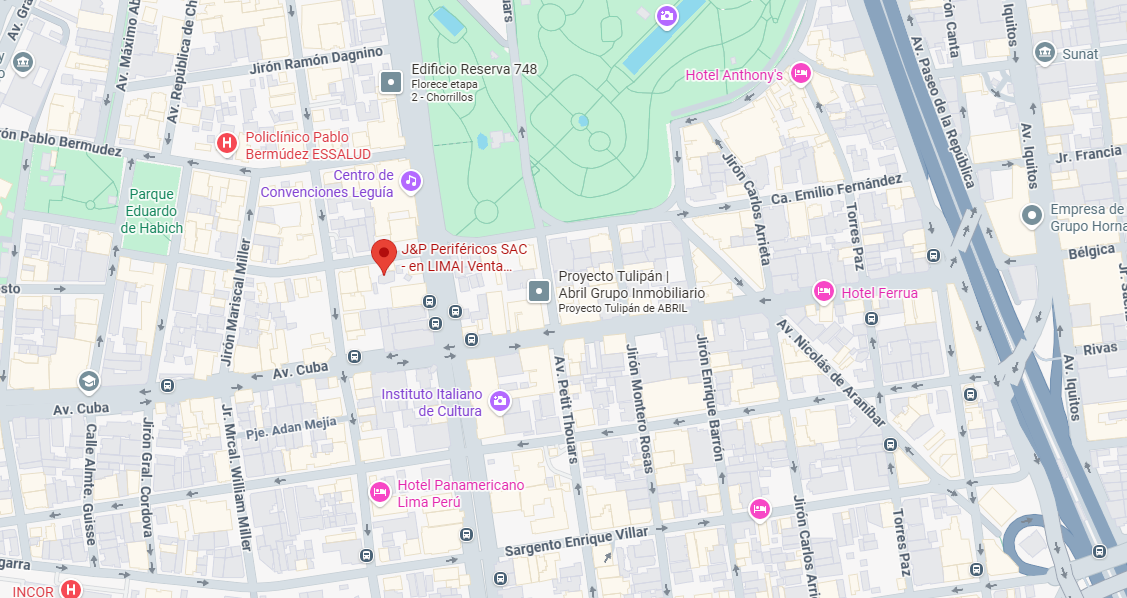
\includegraphics[width=0.8\textwidth]{img/direccion-empres.png}
    
    \vspace{0.4em}
    {\small \textit{Nota.} Ubicación geográfica y mapa vial de la sede central. Adaptado de Google Maps.}
\end{figure}

\FloatBarrier

\section{Misión, Visión, Objetivos y Valores de la Empresa}

\subsection{Misión}
Proporcionar soluciones tecnológicas orientadas a la optimización de los procesos de negocio, facilitando a los clientes métodos efectivos para afrontar los desafíos informáticos empresariales mediante la implementación estratégica y adecuada de las tecnologías de la información.

\subsection{Visión}
Posicionarse como una organización referente en soluciones informáticas, altamente eficiente y rentable, operando bajo estándares de calidad internacional, con un equipo humano calificado y un firme compromiso con el desarrollo sostenible y la preservación del medio ambiente, garantizando la expansión y continuidad del negocio.

\subsection{Objetivos}
% Objetivos a corto plazo
\noindent\textbf{Objetivos a Corto Plazo:}
\begin{itemize}
    \item Consolidar la presencia y posicionamiento comercial en el mercado peruano.
    \item Ampliar la cartera de clientes corporativos e individuales.
    \item Diversificar y actualizar el portafolio de servicios tecnológicos.
    \item Incrementar los índices de satisfacción y fidelización de los clientes.
    \item Optimizar los flujos operativos y tiempos de respuesta en los procesos internos.
\end{itemize}

% Objetivos a largo plazo

\noindent\textbf{Objetivos a Largo Plazo:}
\begin{itemize}
    \item Posicionarse como una empresa líder e innovadora en el sector de tecnologías de la información.
    \item Asegurar la sostenibilidad financiera y la escalabilidad operativa del modelo de negocio.
    \item Contribuir activamente a la transformación digital y al desarrollo tecnológico nacional.
\end{itemize}

\subsection{Valores de la Empresa}
\begin{itemize}
    \item \textbf{Orientación al cliente:} Atención focalizada en los requerimientos específicos de cada cliente, diseñando soluciones a medida que potencien sus procesos de negocio.
    \item \textbf{Innovación continua:} Adopción y aplicación proactiva de tecnologías emergentes para generar valor agregado y dinamismo operativo.
    \item \textbf{Calidad y excelencia:} Compromiso con la entrega de productos y servicios que cumplan con altos estándares técnicos y de rendimiento.
    \item \textbf{Desarrollo humano:} Fomento del crecimiento profesional, técnico y personal del capital humano como pilar del éxito organizacional.
    \item \textbf{Responsabilidad social y ambiental:} Conciencia ambiental y ética corporativa orientada al desarrollo sostenible y buenas prácticas operativas.
\end{itemize}

\section{Producto, Mercado y Cliente}

\subsection{Producto}
La empresa \textbf{J\&P Periféricos S.A.C.} comercializa una gama integral de equipamiento informático, 
suministros y soluciones tecnológicas orientadas tanto al usuario final como al sector corporativo de Lima Metropolitana. Su portafolio de productos y servicios incluye:

\begin{itemize}
    \item \textbf{Laptops y Tablets:} Equipos portátiles para uso personal, profesional y entornos de alto rendimiento.
    \item \textbf{PC y Servidores:} Computadoras de escritorio ensambladas a medida y estaciones de trabajo o servidores para infraestructura empresarial.
    \item \textbf{Impresoras:} Equipos de impresión multifuncionales, térmicos y de inyección o láser para oficina.
    \item \textbf{Monitores:} Pantallas y soluciones de visualización con diversas resoluciones y tecnologías de panel.
    \item \textbf{Componentes para PC:} Placas base, procesadores, memorias, tarjetas de video y unidades de almacenamiento en estado sólido.
    \item \textbf{Accesorios y Repuestos:} Periféricos de entrada/salida, cables estructurados, fuentes de poder y partes de recambio.
    \item \textbf{Soluciones Corporativas:} Servicios de integración tecnológica, mantenimiento preventivo/correctivo y soporte continuo de infraestructura TI.
\end{itemize}

Como parte de la diversificación de su portafolio tecnológico, J\&P Periféricos S.A.C. ha impulsado el desarrollo de un sistema web centralizado para la gestión integral de mesas de ayuda (Help-Desk), control de inventario de activos TI (ITAM) y automatización de soporte técnico presencial y remoto. La empresa proyecta ofrecer esta solución a sus clientes corporativos bajo un modelo modular de servicios tecnológicos. El presente proyecto comprende el desarrollo, despliegue y validación de esta solución en la propia organización; su comercialización externa se plantea como una etapa posterior.

\subsection{Mercado}
El mercado objetivo de la organización se enmarca dentro del sector de las Tecnologías de la Información y Comunicación (TIC). La oferta está dirigida principalmente al segmento empresarial (B2B) y a profesionales independientes (B2C) en Lima Metropolitana que requieren aprovisionamiento de hardware, despliegue de redes, mantenimiento de infraestructura informática y optimización técnica de sus procesos de negocio mediante herramientas digitales.

Para el producto desarrollado en este proyecto, los destinatarios previstos son empresas que requieren integrar la información laboral de sus trabajadores con el procesamiento de nóminas, la revisión de incidencias y la generación de documentos. La cartera existente constituye un ámbito potencial para identificar usuarios interesados, sin que ello implique que todos sus integrantes hayan solicitado o contratado la solución.

\subsection{Cliente}
La cartera de clientes de \textbf{J\&P Periféricos S.A.C.} abarca diversas entidades comerciales, industriales, de salud y servicios profesionales, entre las cuales destacan:

\begin{itemize}
    \item Grupo Enfoque
    \item Sergetic
    \item S\&R Solution Service
    \item Hidromax S.A.C.
    \item Copaco S.A.C.
    \item Fasetron del Perú S.A.C.
    \item Asociación Peruana de Nefrología Pediátrica
    \item Distribuidora Venso S.A.C.
    \item Textiles TBM S.A.C.
\end{itemize}

\section{Organigrama de la Empresa}

\begin{figure}[H]
    \centering
    \captionsetup{justification=centering}
    \caption{Estructura orgánica funcional de J\&P Periféricos S.A.C.}
    \label{fig:organigrama_empresa}
    \vspace{0.2em}
    
    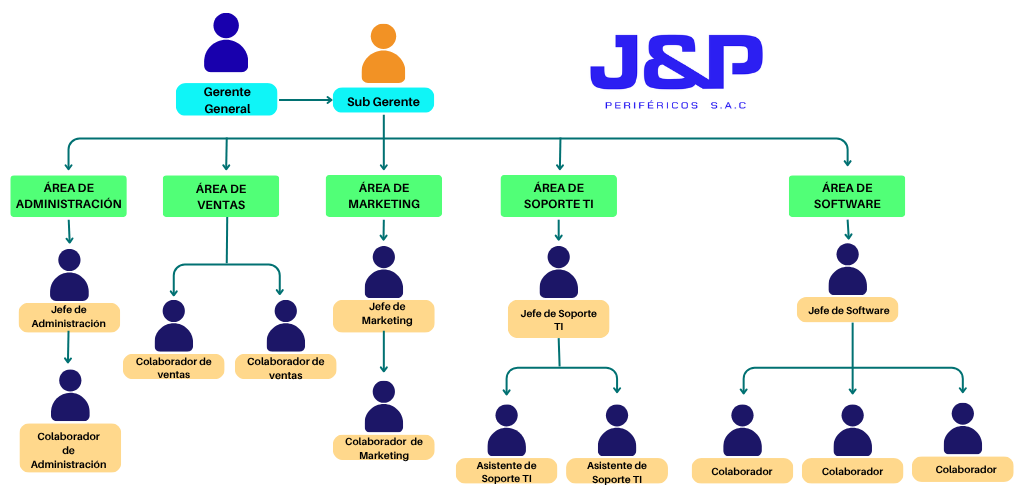
\includegraphics[width=1.0\textwidth]{img/organigrama_empresa.png}
    
    \vspace{0.2em}
    {\small \textit{Nota.} Representación jerárquica y departamental de las áreas funcionales de la empresa. Elaboración propia.}
\end{figure}

\clearpage

\section{Otra Información Relevante de la Empresa donde se desarrolla el Proyecto}

\subsection{Planificación y Gestión de la Entrevista}
Con el propósito de profundizar en el diagnóstico situacional, contrastar la perspectiva estratégica del negocio y sustentar las causas raíz de las deficiencias operativas en la atención de soporte técnico y el control de inventario de activos TI, se diseñó e implementó una entrevista semiestructurada aplicada a los responsables directos de la gestión empresarial y del área de tecnología.

\vspace{0.3cm}
\noindent\textbf{Entrevistado:} Julio Flores Vicuña, \textbf{Gerente General de J\&P Periféricos S.A.C.}
\vspace{0.4cm}

\begin{enumerate}[leftmargin=*, label=\textbf{P\arabic*.}]
    \item \textbf{¿Cuáles son las principales dificultades de gestión interna que ha identificado en la atención de soporte técnico e inventario de TI?}
    
    \textit{Respuesta del Gerente General:} La falta de un canal centralizado de atención. Las solicitudes ingresan por WhatsApp o llamadas informales, lo que genera desorden, solicitudes traspapeladas, retrasos en la respuesta y la imposibilidad de saber qué equipos o licencias tiene asignados cada cliente.

    \item \textbf{¿Qué motivos estratégicos llevaron a la empresa a optar por el desarrollo de un sistema Help-Desk propio en lugar de contratar un software comercial?}
    
    \textit{Respuesta del Gerente General:} Requerimos una solución adaptada a nuestro modelo de negocio multinivel, que integre en una sola plataforma la gestión de tickets, la programación de visitas técnicas in-situ, el control de planes/contratos de soporte y el inventario detallado de hardware y software por cliente.

    \item \textbf{Desde su perspectiva gerencial, ¿cuáles representan los mayores desafíos al momento de supervisar al personal técnico y los servicios prestados?}
    
    \textit{Respuesta del Gerente General:} La ausencia de indicadores de rendimiento (KPIs) en tiempo real. Sin métricas como el tiempo medio de respuesta (MTTA) o resolución (MTTR), es muy difícil evaluar el desempeño de los técnicos y garantizar el cumplimiento de los Acuerdos de Nivel de Servicio (SLA).

    \item \textbf{¿Qué impacto operativo y económico espera que genere la implementación de este sistema Help-Desk?}
    
    \textit{Respuesta del Gerente General:} En lo operativo, estandarizará la atención y eliminará los cruces de horario en las visitas técnicas. En lo económico, reduciremos costos por desplazamientos ineficientes y mejoraremos la retención de clientes corporativos al brindar un servicio transparente y medible.

    \item \textbf{¿Qué necesidades comunes comparten las empresas de su cartera a las que estará orientada la plataforma?}
    
    \textit{Respuesta del Gerente General:} Todas las empresas cliente necesitan trazabilidad sobre las fallas de sus equipos, conocer el historial de mantenimientos y tener la certeza de que sus incidencias críticas se atienden dentro de los tiempos contratados.
\end{enumerate}

\vspace{0.3cm}
\noindent\textbf{Entrevistado:} Jack Huaman, \textbf{Jefe de Soporte Técnico y TI de J\&P Periféricos S.A.C.}
\vspace{0.4cm}

\begin{enumerate}[leftmargin=*, label=\textbf{P\arabic*.}]
    \item \textbf{¿Cuánto tiempo promedio invierte diariamente el equipo en clasificar, asignar y dar seguimiento manual a las solicitudes de soporte?}
    
    \textit{Respuesta del Jefe de TI:} Aproximadamente entre 2 a 3 horas diarias coordinando por mensajes o llamadas, consolidando datos en hojas de cálculo y preguntando al cliente datos básicos del equipo afectado antes de iniciar el diagnóstico.

    \item \textbf{¿Cuáles son los principales cuellos de botella que se presentan al atender un requerimiento sin una base de datos de activos unificada?}
    
    \textit{Respuesta del Jefe de TI:} La falta de antecedentes técnicos. Muchas veces los técnicos van a atender a ciegas sin conocer la configuración, garantías o historial de reparaciones previas del hardware, lo que ocasiona diagnósticos repetitivos y reescritura de informes.

    \item \textbf{¿Cómo se gestiona actualmente la programación de visitas presenciales in-situ y qué problemas ocasiona?}
    
    \textit{Respuesta del Jefe de TI:} Se realiza de forma empírica y verbal. Generando de vez en cuando cruces de horario entre los técnicos, traslados duplicados a la misma zona o demoras en la llegada a clientes con incidencias de prioridad alta.

    \item \textbf{¿Qué errores o inconsistencias son más frecuentes al controlar los contratos y el inventario mediante hojas de cálculo?}
    
    \textit{Respuesta del Jefe de TI:} El desequilibrio de información. Con frecuencia se prestan servicios a equipos que ya no están cubiertos por el plan del cliente o no se registran los componentes o repuestos reemplazados durante la atención.

    \item \textbf{¿Qué herramientas o métricas considera indispensables en el nuevo sistema web?}
    
    \textit{Respuesta del Jefe de TI:} Un panel de tickets por estado y prioridad, un expediente técnico digital por cada activo informático, un calendario de rutas/citas in-situ y un tablero de control con métricas como el tiempo de solución y la satisfacción del cliente.
\end{enumerate}
\cleardoublepage

\chapter[CAPÍTULO II]{PLAN DEL PROYECTO DE INNOVACIÓN / MEJORA / CREATIVIDAD}

\section{Identificación del Problema Técnico de la Empresa}

\subsection{Problema Local de la Empresa}

En la empresa J\&P Periféricos S.A.C., el Área de Soporte Técnico atiende incidencias, solicitudes de asistencia y requerimientos de mantenimiento de equipos informáticos correspondientes a empresas clientes distribuidas en distintas sedes y sucursales. A partir de la entrevista realizada al Gerente General y al Jefe de Soporte Técnico y TI, junto con la revisión de los registros operativos cotidianos, se evidencian diversas dificultades que afectan la continuidad, el orden y la oportunidad del servicio. Esta situación crítica se desglosa a través de una serie de problemáticas encadenadas:

\begin{enumerate}[label=\alph*)]
    \item Desorganización y falta de trazabilidad en la atención de solicitudes recibidas por canales informales como llamadas telefónicas y mensajes de WhatsApp: Los requerimientos de los clientes corporativos ingresan de manera descentralizada y desorganizada a través de canales informales (llamadas telefónicas y chats de mensajería instantánea), sin un formato estandarizado ni categorización previa, aspecto que, de acuerdo con los lineamientos de gestión operativa expuestos por Gonzales Delgado (2025), propicia que las solicitudes queden dispersas y sin registro oficial en los dispositivos del personal técnico.

    \item Inexistencia de un historial centralizado de mantenimientos y expedientes técnicos por equipo, debido al uso de archivos de Excel dispersos y desactualizados: Aunque el control del parque informático se gestiona parcialmente, existe una total ausencia de convenciones de registro estructurado por empresa, sucursal y trabajador. Se emplean hojas de cálculo descentralizadas y desactualizadas, lo cual, tal como señalan Castro y Quispe (2025), obliga a los operadores a realizar búsquedas manuales que incrementan el riesgo de diagnósticos erróneos y reescritura de informes.

    \item Retrasos y cruces de agenda al coordinar visitas técnicas y atenciones presenciales en las instalaciones de los clientes: Actualmente, coordinar las visitas presenciales y asignar técnicos a campo depende exclusivamente de la comunicación empírica y la memoria operativa, una limitación que, según advierten Ramírez y Gómez (2024), desencadena cruces de agenda y traslados duplicados que perjudican la puntualidad del servicio \textit{in-situ}.

    \item Ausencia de indicadores de gestión (KPIs) y reportes consolidados que permitan medir los tiempos de respuesta y el desempeño del área técnica: No existe un núcleo centralizado que supervise el ciclo de vida de los tickets ni evalúe métricas de rendimiento (KPIs), limitación que, en línea con lo evidenciado por Táez Valdiviezo (2021) al contrastar registros manuales frente a una mesa de ayuda estructurada bajo métricas ITIL 4, impide a la gerencia evaluar objetivamente los tiempos de respuesta y resolución, el cumplimiento de los acuerdos de nivel de servicio (SLA) y la productividad del equipo técnico.

    \item Dificultad para controlar y verificar el cumplimiento de los límites de servicio establecidos en los acuerdos con los clientes (SLA): La verificación de la vigencia de los planes contratados, la cantidad máxima de equipos cubiertos y los tiempos máximos de atención comprometidos se realiza de forma manual y fragmentada; esta carencia de control automatizado, tal como advierten Chávez Gomez (2023) y Figueroa Pozo (2023), dificulta priorizar oportunamente las incidencias críticas, provoca que se brinde soporte a activos fuera de cobertura y compromete el cumplimiento formal de los Acuerdos de Nivel de Servicio (SLA).
\end{enumerate}

\vspace{0.8em}

A partir del diagnóstico aplicado y del análisis de Pareto desarrollado en los Anexos, se determina como problema principal: \textit{Desorganización y falta de trazabilidad centralizada en la gestión de solicitudes de soporte técnico y registro de inventario informático multinivel}. En la práctica, esta situación provoca demoras en la asignación y atención de los casos, dificulta ubicar el historial previo de cada activo antes de intervenirlo, genera reprocesos en el seguimiento de las visitas y afecta la percepción de calidad y cumplimiento por parte de los clientes corporativos.

\vspace{0.8em}

\noindent Con base en el levantamiento de información en el área y los resultados del diagnóstico de Pareto, las causas que originan este problema principal se detallan a continuación:

\begin{enumerate}[label=\alph*)]
    \item \textit{La ausencia de una plataforma web centralizada que reemplace la recepción informal de incidencias por mensajería y llamadas}: Según lo manifestado por la jefatura de soporte técnico durante el diagnóstico interno, la ausencia de una plataforma web unificada que reemplace el uso de mensajería informal impide estructurar adecuadamente el flujo de entrada de los requerimientos, generando registros dispersos que anulan cualquier posibilidad de análisis formal de incidencias.
    
    \item \textit{La falta de una base de datos unificada de equipos, componentes y licencias que funcione como expediente técnico confiable}: Al carecer de una base de datos relacional centralizada y normalizada que funcione como expediente técnico por cliente y sucursal, los operadores recurren a búsquedas manuales propensas a errores, degradando la calidad de la información y dificultando los diagnósticos especializados.
    
    \item \textit{La programación empírica y poco estructurada de las rutas y horarios para las visitas técnicas presenciales}: De acuerdo con la coordinación diaria de campo reportada por el área, se carece de una programación lógica para la automatización de citas y asignación optimizada de personal técnico, limitando la coordinación a métodos manuales que incrementan los tiempos de inactividad en las visitas presenciales.
    
    \item \textit{La carencia de tableros analíticos (KPIs) e indicadores de control que permitan evaluar de forma continua los tiempos de atención y la satisfacción del cliente}: La falta de un sistema con backend robusto y modular que centralice las reglas de negocio impide la monitorización en tiempo real de los indicadores de rendimiento y la validación automatizada de contratos, sobrecargando la operación y comprometiendo la calidad del servicio técnico.
\end{enumerate}

\subsection{Problema Nacional}
A nivel nacional, el ecosistema empresarial peruano está conformado de manera predominante por las Micro, Pequeñas y Medianas Empresas (Mipymes), las cuales constituyen el 99,3\% del tejido empresarial formal y concentran el 89,1\% del empleo privado formal (Ministerio de la Producción [PRODUCE], 2025). A pesar de este rol estructural en la economía, gran parte de estas organizaciones presenta un rezago en su madurez tecnológica y digital; operan bajo esquemas empíricos y continúan dependiendo de canales informales de comunicación (como mensajería instantánea) y registros manuales o hojas de cálculo desactualizadas para gestionar sus actividades cotidianas (PRODUCE, 2025). Esta falta de estandarización limita su capacidad operativa y se ve reflejada directamente en el sector tecnológico y de servicios informáticos —como en la empresa J\&P Periféricos S.A.C.—, donde la ausencia de plataformas de gestión centralizadas impide un adecuado control de incidentes y del inventario de activos TI.

Esta problemática refleja una constante preocupante en el sector tecnológico y de servicios informáticos en el Perú. De acuerdo con Altamira (2026), el proceso acelerado de transformación digital en las micro, pequeñas y medianas empresas (PyMEs) tradicionales exige la migración inmediata de sus flujos operativos hacia plataformas de gestión centralizadas para mantener su competitividad en el mercado nacional. No obstante, un gran porcentaje de organizaciones dedicadas al soporte técnico continúa operando mediante esquemas empíricos y no estructurados, apoyados de forma precaria en aplicaciones de mensajería instantánea y registros manuales (Fiberlux Corp, 2025). Esta falta de estandarización limita la capacidad organizativa de las empresas para escalar sus operaciones, controlar adecuadamente los contratos de servicio y brindar una respuesta oportuna frente a incidentes críticos (Vargas, 2024).

En consonancia con este panorama, reportes técnicos advierten que la carencia de una mesa de ayuda unificada y de un inventario informático estructurado en las organizaciones peruanas impide determinar con precisión la causa raíz de las fallas recurrentes de hardware y software (Castro y Quispe, 2025). Esta limitación operativa incrementa sustancialmente los costos por inactividad empresarial (\textit{downtime}), propicia el cruce constante de agendas técnicas en las atenciones presenciales e imposibilita la verificación de los acuerdos de nivel de servicio (SLA) (Ramírez y Gómez, 2024). Ante esta realidad, el sector tecnológico en el Perú demanda soluciones de software accesibles que integren el control jerárquico de activos, la trazabilidad del ticket en tiempo real y la gestión automatizada de visitas técnicas.

En este contexto de aceleración digital, la adopción de herramientas tecnológicas resulta determinante para garantizar la sostenibilidad y competitividad de las empresas peruanas. Al respecto, Alvarado (2023) sostiene que la transformación digital orientada a la automatización de procesos y la simplificación operativa no solo incrementa la eficiencia y reduce costos, sino que disminuye drásticamente los tiempos de ciclo en la atención de requerimientos del cliente, factor crítico para fortalecer la lealtad e incrementarla satisfacción en el mercado nacional. Sin embargo, la falta de integración de plataformas accesibles y estructuradas en el sector de servicios TI impide que muchas organizaciones locales reduzcan sus tiempos de respuesta, limitando su capacidad para ofrecer un servicio transparente y de calidad global.

Aunado a lo anterior, las deficiencias en la gestión de servicios y el tiempo de inactividad operativo generan pérdidas financieras críticas en el tejido empresarial del país. De acuerdo con un informe especializado publicado por Tricentis (2025), el 40\% de las organizaciones peruanas estima pérdidas anuales que oscilan entre US\$\ 1 millón y US\$\ 5 millones, mientras que otro 42\% reporta pérdidas de entre US\$\ 500 mil y US\$\ 1 millón a causa de fallas de software y la necesidad de mantenimiento correctivo constante. Esto demuestra que la falta de herramientas automatizadas y de una trazabilidad centralizada de incidencias en las empresas locales no solo provoca retrasos operativos, sino que se convierte en un riesgo financiero latente que compromete la continuidad del negocio.


\subsection{Problema Internacional}

A nivel global, la gestión de servicios de tecnología de la información (ITSM) enfrenta desafíos análogos vinculados con la madurez operativa y la automatización de procesos. Según estudios desarrollados por el Service Desk Institute (2024), las mesas de ayuda internacionales priorizan la eliminación paulatina del trabajo manual mediante la incorporación de flujos de trabajo automatizados para la recepción, clasificación, asignación y seguimiento de requerimientos. La dependencia de canales de atención informales es catalogada a nivel internacional como uno de los factores de mayor riesgo para la continuidad del negocio, ya que incrementa la insatisfacción del cliente y genera cuellos de botella en el soporte de primer y segundo nivel (Gartner, 2025).

Por su parte, diversas investigaciones y experiencias internacionales evidencian que operar sin herramientas centralizadas de Help Desk ni métricas formales de servicio dificulta el control de los tiempos de respuesta y resolución de incidencias, mientras que la adopción de plataformas estructuradas bajo métricas ITIL 4 permite reducir dichos tiempos y mejorar el seguimiento operativo (Táez Valdiviezo, 2021). La ausencia de herramientas analíticas centralizadas impide a la gerencia evaluar objetivamente el desempeño del personal técnico y validar el cumplimiento de los contratos de soporte. Asimismo, la adopción de plataformas basadas en buenas prácticas reduce significativamente las horas de inactividad operativa y optimiza la atención de incidencias en organizaciones de diversa índole (Velasco Castro, 2023; Figueroa Pozo, 2023).

En esta misma línea, Díaz Hidalgo (2024) demuestra en su estudio para la Cruz Roja Ecuatoriana que la alta demanda de soporte y el uso de herramientas obsoletas o al límite de su capacidad generan saturación operativa y cuellos de botella en las áreas de tecnología; por ello, la implementación de soluciones Help-Desk en la nube bajo marcos como ITIL permite mitigar estas deficiencias, estabilizando el servicio y optimizando de forma integral los procesos de TI. En consecuencia, la tendencia internacional se orienta hacia la adopción de plataformas web robustas y multitenant que integren en un único entorno la comunicación instantánea, el inventario jerárquico de activos y la analítica de servicios.

A nivel internacional, la gestión ineficiente de las solicitudes y requerimientos en las áreas de tecnología de la información constituye un obstáculo crítico para la productividad institucional. Diversas organizaciones enfrentan desafíos análogos al carecer de herramientas automatizadas para el soporte técnico. Por ejemplo, en la empresa Técnica Avícola S.A. de Pacasmayo (Perú), la ausencia de un sistema de atención informática generaba deficiencias sustanciales en el departamento de TI, lo que motivó la implementación de una plataforma de tipo \textit{Help Desk} para optimizar el registro y la resolución de incidencias (Gonzales, 2016).

Asimismo, en el sector empresarial peruano, la empresa Telvicon evidenció problemas operativos similares relacionados con el manejo desorganizado de sus servicios técnicos, situación que requirió la adopción de un \textit{Service Desk} bajo el marco de trabajo ITIL para mejorar los tiempos de respuesta y la calidad del servicio (Rodríguez y Falcón, 2019). De manera análoga, en el contexto ecuatoriano, la Universidad Politécnica Salesiana analizó el impacto negativo de los métodos tradicionales de soporte, concluyendo que la falta de herramientas centralizadas deteriora el desempeño del área técnica y alarga los tiempos de atención a los usuarios (Ponce y Samaniego, 2015). 

Estas experiencias internacionales demuestran que el uso de procesos manuales o informales en la gestión de incidencias provoca congestión operativa, retrasos y pérdida de información, evidenciando la necesidad imperativa de implementar sistemas web especializados que automaticen el flujo de trabajo en el soporte tecnológico.

\vspace{0.8em}

\subsection{Formulación del Problema}

\noindent \textbf{Problema General}

\vspace{0.5em}

¿De qué manera la implementación de un sistema web Help-Desk centralizado optimiza la gestión de atenciones técnicas y el registro de cambios de hardware y software en equipos multinivel para la empresa J\&P Periféricos S.A.C.?

\vspace{1.2em}

\noindent \textbf{Problemas Específicos}

\begin{itemize}[leftmargin=1.27cm]
    \item ¿De qué forma la asignación automatizada de tickets influye en la reducción de retrasos ocasionados por la gestión manual e informal de solicitudes?
    
    \item ¿Cómo la integración de un módulo de inventario informático por cliente impacta en la trazabilidad del expediente técnico de hardware y software?
    
    \item ¿De qué manera la programación de citas y soporte presencial reduce los cruces de horario y la descoordinación en las visitas \textit{in-situ}?
    
    \item ¿De qué forma el control digital de planes y contratos de soporte contribuye al cumplimiento de los límites de servicio acordados?
    
    \item ¿Cómo el flujo estandarizado de atención favorece el seguimiento y resolución oportuna de los tickets escalados a nivel técnico?
    
    \item ¿De qué manera la provisión de tableros con indicadores de rendimiento (KPIs) permite medir los tiempos de respuesta y la satisfacción del cliente?
\end{itemize}

\newpage

\section{Objetivo del Proyecto de Innovación}

\subsection{Objetivo General}

Desarrollar e implementar un Sistema Web Help-Desk Centralizado para la gestión del servicio de soporte técnico y el control de inventario de activos TI en la empresa J\&P Periféricos S.A.C., con el fin de optimizar los tiempos de atención, garantizar la trazabilidad de los recursos informáticos y mejorar la satisfacción del cliente.

\vspace{0.8em}

\subsection{Objetivos Específicos}

\begin{itemize}[leftmargin=1.27cm]
    \item Automatizar la recepción y asignación de solicitudes de soporte, mediante un módulo de gestión de tickets que elimine los retrasos del canal manual e informal.
    
    \item Implementar un módulo de gestión de expedientes e inventarios de TI (hardware y software), parametrizado por empresa, sucursal, área y trabajador para garantizar la trazabilidad de los equipos.
    
    \item Integrar un módulo de agendamiento y programación de citas presenciales, para optimizar la coordinación y asignación del personal de soporte \textit{in-situ}.
    
    \item Desarrollar un módulo de control digital de planes y contratos de soporte, que valide de forma automatizada los límites de cobertura y Acuerdos de Nivel de Servicio (SLA) vinculados a cada cliente.
    
    \item Estandarizar el procedimiento de derivación y escalamiento de tickets, para asegurar el seguimiento continuo y la resolución oportuna de las atenciones a nivel técnico.
    
    \item Construir un módulo de métricas y tableros de control (KPIs), para evaluar el Tiempo Medio de Resolución (MTTR), medir los tiempos de respuesta y monitorear la satisfacción del cliente.
\end{itemize}

\section{Antecedentes del Proyecto de Innovación / Mejora / Creatividad (investigación realizada)}

\subsection{Antecedentes Nacionales}

En esta tesis de pregrado de la Universidad César Vallejo en la Escuela Profesional de Ingeniería de Sistemas, sustentada por Fonseca Calcin (2025), titulada ``Help desk para la atención de incidencias del área de soporte técnico de una asociación educativa cultural'', se señala como problema principal que la falta de un Help Desk estructurado expone la información institucional a riesgos por virus y amenazas informáticas en la red, dificultando la detección y respuesta oportuna ante incidentes de seguridad, lo que genera desorden, demoras en la solución de fallas y afecta la satisfacción de los usuarios. El objetivo principal fue implementar un sistema de Help Desk para optimizar la gestión de incidencias y reducir los riesgos de la información ante la amenaza de virus e infecciones informáticas en las redes de la institución. La metodología aplicada correspondió a una investigación básica y cuantitativa sobre sistemas de Help Desk y herramientas de gestión tecnológica actuales para resolver problemas de atención de incidencias e inseguridad de la información. Como resultado, se obtuvo que el Help Desk explica el 69.4\% de la mejora en la atención de incidencias, logrando una correlación positiva fuerte que optimiza la detección, registro y respuesta oportuna ante amenazas y fallas en la red. Se concluyó que, a pesar de las constantes amenazas informáticas, la implementación del Help Desk permite combatir los riesgos y proteger la información del servidor mediante una atención de incidencias organizada, rápida y efectiva.

\vspace{0.8em}

En esta tesis de Maestría de la Universidad César Vallejo, sustentada por Villalva Mendivil (2022), titulada ``Sistema Helpdesk en la Gestión de Incidencias del Área de TI en una Empresa de Telecomunicaciones, Lima, 2022'', se expone como problemática que la ausencia de un sistema Helpdesk estructurado generaba desorden en el registro de fallas y demoras prolongadas en la atención de TI, lo que obligaba a realizar desplazamientos innecesarios para problemas menores, afectando el cumplimiento de los tiempos de respuesta (SLA), interrumpiendo la operatividad y reduciendo la satisfacción de los usuarios. El objetivo fue implementar un sistema Helpdesk para mejorar la gestión de incidencias en el área de TI de la empresa TELEGEN PERU SAC mediante un diseño preexperimental. La metodología empleó una investigación aplicada de enfoque cuantitativo y diseño preexperimental de corte longitudinal, evaluando la implementación mediante fichas de registro para medir la mejora en los indicadores de atención, solución en primer nivel, cumplimiento de SLA y tiempos de respuesta. Como resultado, se obtuvo que la implementación incrementó la atención de incidencias del 63.74\% al 88.68\% y la resolución en primer nivel del 48.52\% al 93.57\%, reduciendo sustancialmente los tiempos de respuesta y mejorando de manera significativa el cumplimiento de los SLA. Se concluyó que el sistema Helpdesk optimiza significativamente la gestión de incidencias en el área de TI, permitiendo reducir los tiempos de respuesta y garantizar una atención organizada, rápida y efectiva a través del incremento en la resolución de primer nivel y el cumplimiento de los SLA.

\vspace{0.8em}

En esta tesis de la Universidad Peruana los Andes, presentada por Chávez Cotera (2022), titulada ``Implementación de un Sistema de Help Desk para Mejorar la Gestión de Incidencias del Parque Informático en el Gobierno Regional Junín'', se expone como problemática que en el Gobierno Regional Junín la gestión de incidencias se registraba mediante cuadernos de control manuales o en hojas de cálculo al final de cada semana. Esta falta de automatización generaba una brecha significativa en la atención, atendiéndose solo un promedio del 74\% de los incidentes y asignándose el 80\% de los mismos, lo cual afectaba la calidad de atención y provocaba insatisfacción en los usuarios e ineficiencia en horas-hombre. El objetivo fue determinar la influencia de un sistema Help Desk en la mejora de la gestión de incidencias del parque informático mediante un diseño preexperimental. La metodología empleó una investigación aplicada de nivel explicativo con diseño preexperimental (pre-test y post-test) bajo la metodología RUP, aplicando fichas de registro y un muestreo probabilístico de reportes diarios. Como resultado, se obtuvo que la implementación del sistema Help Desk incrementó el porcentaje de incidencias atendidas del 74.12\% al 74.99\% y el porcentaje de incidencias asignadas del 80.26\% al 83.75\%, mejorando el control y la canalización operativa de los requerimientos. Se concluyó que la implementación del sistema Help Desk optimiza significativamente la gestión de incidencias del parque informático en el Gobierno Regional Junín, superando las limitaciones de los registros manuales y garantizando una atención más organizada y eficiente.

\vspace{0.8em}

En esta tesis de Maestría de la Universidad César Vallejo, sustentada por Figueroa Santander (2022), titulada ``Aplicación ITIL en la Gestión de Incidencias en el Área de Informática de una Empresa de Turismo, Lima 2022'', se expone como problemática que antes de aplicar la metodología ITIL, la empresa presentaba graves deficiencias en la atención de fallas informáticas debido a la falta de un alineamiento adecuado y el seguimiento de procesos. Esto generaba retrasos, cuellos de botella en la recepción de solicitudes, acumulación de incidencias no resueltas y un elevado tiempo de resolución, afectando la calidad del servicio brindado a los usuarios y clientes. El objetivo fue determinar la influencia de la aplicación ITIL en la gestión de incidencias del área de informática de una empresa de turismo en Lima mediante un diseño preexperimental. La metodología correspondió a una investigación aplicada de nivel explicativo y enfoque cuantitativo, con un diseño preexperimental de corte longitudinal. Mediante fichas de observación sobre una muestra probabilística de 215 incidencias (distribuidas en 30 registros), se evaluó el comportamiento de los indicadores de resolución y tiempos antes y después del tratamiento experimental. Como resultado, se obtuvo que la implementación de las buenas prácticas de ITIL incrementó el promedio de incidencias resueltas del 56.52\% al 70.13\% y redujo el porcentaje de incidencias no resueltas del 43.47\% al 29.86\%. Asimismo, el tiempo promedio de resolución de incidencias se redujo sustancialmente de 38.36 a 12.58 minutos. Se concluyó que la aplicación de ITIL influye positivamente en la gestión de incidencias del área de informática, permitiendo optimizar el flujo de trabajo, reducir los tiempos de espera y garantizar una solución organizada, rápida y oportuna a los requerimientos técnicos de la empresa.

\vspace{0.8em}

En esta tesis de Maestría de la Universidad César Vallejo, sustentada por Mendoza Lizana (2023), titulada ``ITIL-V.4 en la Gestión de Incidencias para el área de service desk en una empresa privada de servicios, Lima 2023'', se presenta como problemática que en la entidad de servicios estudiada el proceso de reporte y atención de incidencias resultaba poco fluido, requiriendo que los usuarios enviaran correos a la mesa de ayuda para luego ser evaluados y escalados a distintas áreas para la validación de permisos. La falta de una metodología o flujo estandarizado generaba demoras significativas en la resolución de los requerimientos e incidentes reportados. El objetivo general fue determinar cómo influye ITIL V.4 en la gestión de incidencias para el área de service desk en una empresa privada de servicios en Lima durante el año 2023. La investigación fue de tipo básica, nivel descriptivo-explicativo, con un enfoque cuantitativo y un diseño no experimental, transversal y correlacional, sobre una población censal de 65 colaboradores mediante la técnica de la encuesta. Como resultado, se obtuvo una relación positiva muy alta del 93.7\% entre ITIL V.4 y la gestión de incidencias, influyendo en un 88.9\% en la solución de problemas, un 85.6\% en la calidad del servicio y un 90.1\% en la satisfacción del usuario. Se concluyó que la adopción del marco de buenas prácticas ITIL V.4 influye de manera directa y significativa en la gestión de incidencias del área de service desk, optimizando el flujo de trabajo, reduciendo los tiempos de atención y elevando la calidad del servicio técnico y la satisfacción general de los usuarios.

\vspace{1.2em}

\subsection{Antecedentes Internacionales}

En esta tesis de maestría de la Universidad Técnica del Norte, sustentada por Táez Valdiviezo (2021), titulada ``Implantación de una herramienta cloud Help Desk para mejorar el tiempo de respuesta troubleshooting de red basado en las métricas ITIL4 para el Gobierno Autónomo Descentralizado Municipal del Cantón La Joya de los Sachas'', se señala como problemática que la gestión tradicional de incidencias y soporte técnico —apoyada en registros manuales en hojas de cálculo y comunicación dispersa— generaba retrasos en la atención, tiempos de respuesta y resolución prolongados, así como dificultades para controlar el cumplimiento de los niveles de servicio (SLA). El objetivo general fue implantar una herramienta cloud Help Desk basada en métricas ITIL 4 para mejorar los tiempos de respuesta en el troubleshooting y soporte técnico. La metodología correspondió a un enfoque cuantitativo de tipo aplicado y comparativo (antes y después), contrastando los registros históricos previos (en hojas de cálculo) frente a los tiempos operativos registrados tras la puesta en marcha de la plataforma ServiceDesk Plus en el área administrativa y técnica. Como resultado, se obtuvo una reducción del tiempo promedio de primera respuesta de 10,03 a 4,32 minutos (49,13\% de mejora promedio reportada por el autor) y una disminución del tiempo promedio de resolución de 108,28 a 98,27 minutos (14,46\% de mejora promedio reportada por el autor), además de una mejora en los tiempos por nivel de SLA de 104,07 a 92,40 minutos (11,64\% de mejora promedio reportada por el autor), consolidando un 25,08\% de mejora general promedio en los tiempos de atención. Se concluyó que la adopción de una herramienta Help Desk estructurada bajo métricas ITIL 4 optimiza los tiempos de respuesta y resolución, formaliza el seguimiento de incidencias y brinda mayor control operativo frente a los registros manuales.

\vspace{0.8em}

En esta tesis de la Universidad Politécnica Salesiana, sustentada por Díaz Hidalgo (2024), titulada ``Diseño de software de Help Desk en la nube basado en ITIL para la Cruz Roja Ecuatoriana'', sse identifica como problemática la saturación de la plataforma local de mesa de ayuda (Spiceworks Desktop) debido al alto volumen diario de tickets y al agotamiento de la capacidad y vida útil del servidor donde se alojaba, lo que afectaba el rendimiento y los tiempos de atención del área de TI. El objetivo general fue diseñar e implementar un servicio de Help Desk en la nube basado en las buenas prácticas de ITIL para optimizar recursos y mejorar los tiempos de respuesta del soporte técnico. La metodología aplicó un enfoque inductivo, analítico y experimental bajo modalidad bibliográfica y de campo, sin muestreo poblacional por estar dirigido directamente al departamento de TI de la institución, definiendo roles de prioridad, una fórmula de criticidad de incidentes y la migración del historial de tickets en formato JSON hacia Spiceworks Cloud. Como resultado, se logró migrar el historial conservando los identificadores y comentarios de los tickets, eliminar los costos de servidor físico, licenciamiento y alojamiento en data center, y disponer de un dashboard estadístico para monitorear tickets abiertos/cerrados, categorías y tiempos promedio de primera respuesta y cierre. Se concluyó que el uso de una mesa de ayuda en la nube alineada a ITIL libera infraestructura local, estandariza la atención según la criticidad del incidente y facilita el control operativo de los tiempos de respuesta mediante indicadores visuales.

\vspace{0.8em}

En esta tesis de la Universidad Pública de El Alto, sustentada por Velasco Castro (2023), titulada ``Sistema de Ticket especializado para la Gestión de incidencias en Soporte Técnico'', se expone como problemática que en el gobierno municipal de Achocalla el registro de incidencias se realiza de forma manual mediante formularios preimpresos, ocasionando pérdida de tiempo e información, así como demoras en el registro y atención de los requerimientos. El objetivo general fue desarrollar un sistema de ticket especializado para la gestión de incidencias en soporte técnico que permita el registro automatizado y eficiente de incidencias de hardware y software, mejorando la calidad y rapidez del servicio mediante metodologías ágiles. La investigación adoptó un razonamiento inductivo con enfoque cualitativo, empleando observaciones directas, revisión de formularios preimpresos y entrevistas semiestructuradas, además de validaciones mediante pruebas de caja blanca y negra, métricas ISO/IEC 9126, controles ISO/IEC 27002 y estimación de esfuerzo con el modelo COCOMO II. Como resultado, la implementación demostró un alto nivel de calidad bajo la norma ISO/IEC 9126 con una usabilidad del 95\%, garantizando la confidencialidad, integridad y disponibilidad mediante cifrado y control de accesos por roles. Se concluyó que el sistema web HelpDesk optimiza significativamente la gestión de incidencias en el área de TI, superando las limitaciones de los procesos manuales y garantizando una atención organizada, rápida y efectiva a través del incremento en la eficiencia operativa, el control centralizado de los requerimientos y una usabilidad sobresaliente para los usuarios finales.

\vspace{0.8em}

En esta tesis de pregrado de la Universidad Estatal Península de Santa Elena, sustentada por Figueroa Pozo (2023), titulada ``Estructura de una mesa de ayuda en el departamento de TI del Ministerio de Inclusión Económica y Social con el fin de mejorar el control de incidentes basadas en la metodología ITIL V3'', se expone como problemática que la falta de una mesa de ayuda estructurada y la presencia de un solo encargado para atender a más de 350 usuarios generaban desorden, cuellos de botella y demoras prolongadas en la atención de TI, gestionando las incidencias sin priorización clara ni seguimiento formal al carecer de un catálogo de servicios definido y del marco ITIL v3. El objetivo general was implementar una propuesta de estructuración de la mesa de ayuda basada en las buenas prácticas de ITIL v3 para el departamento de TI del Ministerio de Inclusión Económica y Social, con el fin de optimizar el control de incidentes, reducir los tiempos de atención y mejorar la prestación del servicio. La metodología presentó un enfoque mixto (cuantitativo y cualitativo) de tipo descriptivo y no experimental, empleando encuestas dirigidas al personal administrativo para medir el nivel de satisfacción, entrevistas estructuradas al responsable de TI y observación directa para diagnosticar el flujo de atención y el volumen de incidentes bajo el marco de ITIL v3. Como resultado, se diseñó la estructura de la mesa de ayuda alineada a ITIL v3, definiendo un catálogo de servicios, flujos de atención y niveles de escalado claros; además, la propuesta demostró que, al estandarizar los procesos de recepción y priorización, se eliminan los cuellos de botella, registrando y controlando el 100\% de los incidentes y mejorando los tiempos de respuesta y la satisfacción de los usuarios. Se concluyó que la reestructuración de la mesa de ayuda bajo ITIL v3 optimiza significativamente la gestión de incidentes al estandarizar los procesos de recepción, priorización y escalado, mientras que la incorporación de un catálogo de servicios categorizado y acuerdos de nivel de servicio (SLA) mejora el tiempo de respuesta, elimina el desorden operativo y eleva la calidad percibida del servicio por parte de los usuarios institucionales.

\vspace{0.8em}

En esta tesis de pregrado de la Facultad de Tecnología Franca Dr. Thomaz Novelino, sustentada por Teixeira Ferreira y Knoll Ricardo (2026), titulada ``HelpSynk - Sistema de gerenciamento de tickets: Solução freemium para equipes de TI com atendimento ao cliente'', se plantea como problemática que las pequeñas empresas y equipos internos de TI enfrentan serias dificultades en la gestión de solicitudes debido a la falta de herramientas centralizadas, recurriendo a canales informales (como correo electrónico o mensajería instantánea), lo que genera saturación, duplicación de requerimientos, pérdida de información y una nula trazabilidad en los costos y repuestos utilizados por sector. El objetivo general fue proyectar y desarrollar el sistema web ``HelpSynk'' para la gestión centralizada de tickets de soporte técnico en pequeñas organizaciones, optimizando el flujo de atención, reduciendo los tiempos de respuesta y permitiendo el control de costos operativos por sector. La metodología aplicó un desarrollo de software ágil e incremental, basado en elicitación de requisitos (entrevistas semiestructuradas, encuestas a usuarios finales y análisis comparativo de mercado), además de modelado de procesos en BPMN y diagramas UML (casos de uso, clases, actividades, estados y secuencia). Como resultado, se logró la implementación exitosa de la plataforma web HelpSynk, validada mediante pruebas piloto en un ambiente real con la empresa Hidromar, demostrando una reducción de hasta el 40\% en el tiempo de clasificación de solicitudes, eliminando el registro de llamadas duplicadas y ofreciendo un panel de control interactivo con exportación de reportes a Excel, detallando los costos de repuestos y servicios por atención. Se concluyó que la implementación de un sistema Help Desk propio centraliza de manera eficiente las atenciones informáticas en pequeñas y medianas organizaciones.

\vspace{1.2em}

\subsection{Artículos Científicos}

En el artículo científico publicado por Vargas Calapucha y Romero Licuy (2026), titulado ``Sistema web de gestión de mantenimiento y baja de equipos del Instituto Superior Tecnológico Tena'', se plantea como problemática que el uso de métodos manuales, registros físicos y hojas de cálculo para la gestión de equipos tecnológicos provocaba pérdida de información, demoras en la atención de fallas y serias dificultades en la trazabilidad de los activos. El objetivo principal fue desarrollar una plataforma web para la gestión del mantenimiento y baja de equipos tecnológicos en el Instituto Superior Tecnológico Tena, permitiendo centralizar la información, automatizar procesos y generar reportes para la toma de decisiones. La metodología correspondió a una investigación aplicada con enfoque mixto, empleando el marco ágil SCRUM para el desarrollo iterativo y flexible del software web. Como resultado, se logró la construcción e implementación de la plataforma web, evidenciando una mejora significativa en la organización del mantenimiento, la seguridad de los datos y la eficiencia operativa de los servicios técnicos e institucionales. Se concluyó que el desarrollo del sistema web optimizó los recursos tecnológicos e impulsó la transformación digital del instituto, resolviendo la pérdida de información y garantizando un control eficiente del ciclo de vida de los activos.

\vspace{0.8em}

En el artículo científico de Gonzales Delgado (2025), titulado ``Sistema informático HelpDesk en la calidad de servicio TI de la Dirección Regional de Transportes y Comunicaciones - Tarapoto, 2025'', se analiza la problemática asociada a las limitaciones en la gestión de incidencias registradas antes de la solución (97 no resueltas y 267 horas de tiempo total de resolución), provocando que la calidad del servicio de TI se concentrara en niveles medio (58.2\%) y bajo (41.8\%). El objetivo fue determinar de qué manera el uso de un sistema informático HelpDesk mejora la calidad del servicio de TI en la Dirección Regional de Transportes y Comunicaciones de San Martín -- Tarapoto, 2025. La metodología fue de tipo aplicada con un diseño preexperimental de corte longitudinal; la población y muestra estuvo conformada por 67 usuarios del servicio de TI, empleando la encuesta y la observación mediante cuestionarios y guías de observación. Como resultado, tras implementar el sistema GLPI basado en ITIL 4, las incidencias resueltas aumentaron a 432 (+18\%), las no resueltas cayeron a 32 (-67\%) y el tiempo de resolución bajó a 178 horas (-33\%); asimismo, la calidad alta alcanzó el 52.2\% y se eliminó por completo el nivel bajo (0.0\%). Se concluyó que el uso del sistema informático HelpDesk mejora significativamente la calidad del servicio TI ($p < 0.05$) en todas sus dimensiones (fiabilidad, capacidad de respuesta, seguridad, empatía y elementos tangibles).

\vspace{0.8em}

En el artículo científico publicado por Arteaga y Astudillo León (2012), titulado ``Sistema de Helpdesk mediante el uso de entorno web'', se expone como problemática la falta de un canal web accesible e inmediato para el reporte de incidentes informáticos durante la jornada laboral, sumada a la ausencia de constancia formal en las solicitudes y la falta de un registro estructurado de soluciones técnicas. El objetivo general fue proporcionar un sistema web Helpdesk rápido y sencillo que permita a los empleados solicitar soporte con respaldo vía correo electrónico, consultar la base de conocimiento y calificar la atención recibida. La metodología correspondió a una investigación aplicada de nivel descriptivo, orientada al desarrollo de una plataforma web con integraciones de notificaciones por correo, bitácora de soluciones técnicas y módulos de evaluación de satisfacción. Como resultado, se implementó el sistema web permitiendo el registro centralizado de solicitudes, la emisión de respaldos por correo, la consulta eficiente de la base de conocimiento por parte de soporte y la calificación del nivel de satisfacción por los usuarios. Se concluyó que el sistema de Helpdesk optimiza la atención de incidentes informáticos, garantizando trazabilidad en los requerimientos, reduciendo tiempos mediante la bitácora de soluciones y asegurando la mejora continua del servicio.

\vspace{0.8em}

En el artículo científico publicado por Chávez Gomez (2023), titulado ``Implementación del Sistema de Help Desk Para la Gestión de Incidentes en la Central de Tecnologías de Información de una Entidad del Estado, 2023'', se expone como problemática la desorganización en la atención de solicitudes técnicas, los tiempos elevados de respuesta, la falta de centralización en la comunicación con soporte y las dificultades para dar cumplimiento a los Acuerdos de Nivel de Servicio (SLA). El objetivo general fue implementar un sistema de Help Desk para optimizar la gestión de incidentes, problemas y consultas de usuarios en la Central de Tecnologías de Información de una Entidad del Estado. La metodología correspondió a una investigación aplicada de diseño preexperimental basada en buenas prácticas de ITIL v4, orientada a la estandarización de flujos de trabajo de ticketing y la automatización del soporte técnico. Como resultado, se logró la estandarización de procesos, la recopilación centralizada de datos para análisis detallados, la mejora en la colaboración interna del equipo técnico y una atención más rápida de requerimientos. Se concluyó que el sistema Help Desk contribuye de manera efectiva a la gestión de incidentes, asegurando la calidad en el servicio al cliente, el cumplimiento de los SLA y la mejora continua de los servicios tecnológicos.

\vspace{0.8em}

En el artículo científico publicado por Loza Calderon (2024), titulado ``Revisión de un sistema web helpdesk para la gestión de incidencias de la infraestructura tecnológica en el Hotel GHL Lago Titicaca Puno 2024'', se analiza como problemática las deficiencias en el seguimiento y monitoreo de incidencias del sistema Helpdesk actual del hotel, evidenciadas por la falta de herramientas en tiempo real y la limitada accesibilidad de los usuarios a la información relevante. El objetivo general fue revisar e implementar mejoras en el sistema web Helpdesk del Hotel GHL Lago Titicaca para optimizar la gestión de incidencias tecnológicas, elevar la eficiencia operativa y mejorar la satisfacción del cliente. La metodología adoptó una investigación de enfoque sistemático y aplicado, centrada en el diagnóstico del proceso de soporte técnico, la integración de herramientas analíticas de diagnóstico en tiempo real y la evaluación periódica de los tiempos de respuesta. Como resultado, se incorporaron herramientas de monitoreo en tiempo real, reportes analíticos avanzados y herramientas de diagnóstico, logrando reducir significativamente los tiempos de respuesta/resolución e identificar patrones de fallas para una gestión preventiva. Se concluyó que la optimización del sistema web Helpdesk mejoró la operatividad del hotel y la experiencia de los huéspedes mediante una toma de decisiones más estratégica basada en datos, recomendando evaluaciones periódicas y capacitación continua del personal.

\section{Justificación del Proyecto de Innovación / Mejora / Creatividad}

\subsection{Justificación Legal}
La implementación del sistema HelpDesk para la empresa J\&P Periféricos S.A.C. responde a la necesidad de adecuar las operaciones de soporte técnico al marco normativo peruano sobre gestión y protección de datos. El tratamiento de información de clientes, contactos y credenciales exige el cumplimiento estricto de la \textbf{Ley N.° 29733 (Ley de Protección de Datos Personales)} y su Reglamento (D.S. N.° 003-2013-JUS). La centralización de las incidencias en una base de datos relacional segura elimina el manejo informal de información en aplicaciones de mensajería o correos personales no auditables, reduciendo el riesgo de filtraciones o pérdidas.

Asimismo, la plataforma contempla controles de acceso basados en roles (RBAC), autenticación mediante tokens JWT y registro de auditoría (\textit{logs}), alineándose con las exigencias de la \textbf{Ley N.° 30096 (Ley de Delitos Informáticos)} para prevenir accesos no autorizados, alteración de datos o fugas de información. Por último, la gestión formal de Acuerdos de Nivel de Servicio (SLA) dentro del sistema brinda soporte normativo a los contratos de atención, siguiendo los lineamientos de la norma \textbf{NTP-ISO/IEC 27001} en cuanto a trazabilidad y seguridad en la entrega de servicios de TI.

\subsection{Justificación Social}
En el ámbito organizacional, la adopción de una plataforma estructurada mejora directamente la calidad de vida laboral del equipo de soporte y fortalece la relación con los clientes. En la operatividad actual, la atención empírica genera sobrecarga de trabajo, duplicación de esfuerzos y cruces de horario en las visitas técnicas, lo que incrementa el estrés laboral y dificulta el seguimiento de las solicitudes.

El sistema HelpDesk organiza y prioriza los tickets de atención, facilitando la programación transparente de visitas \textit{in-situ} y soportes remotos. Esto optimiza el uso del tiempo técnico, reduce desplazamientos innecesarios y fomenta un entorno de trabajo más equitativo y ordenado. Por su parte, las empresas cliente obtienen mayor visibilidad sobre el estado de sus requerimientos, lo que construye una relación de confianza mutua basada en la previsibilidad y la calidad del servicio.

\subsection{Justificación Teórica}
El proyecto se fundamenta en la aplicación práctica de marcos de trabajo y estándares internacionales de la Gestión de Servicios de Tecnologías de la Información (ITSM). En el plano operativo, se toman como referencia los flujos de gestión de incidentes, peticiones de servicio y activos de \textbf{ITIL v4}, transformando un proceso que se ejecutaba de forma empírica en una operación estandarizada, medible y trazable.

Desde la perspectiva del desarrollo de software, la propuesta valida la implementación de una arquitectura desasociada moderna. El backend adopta el framework \textit{NestJS} basado en TypeScript con arquitectura modular e inyección de dependencias, respaldado por \textit{MySQL} para datos transaccionales, \textit{MongoDB} para el almacenamiento del historial de chats y \textit{Redis} con \textit{WebSockets} para la comunicación en tiempo real. Esta combinación demuestra teóricamente cómo el uso de arquitecturas escalables y tecnologías web consolidadas mejora la mantenibilidad, estabilidad y rendimiento del software empresarial en procesos de soporte técnico.


\section{Marco Teórico y Conceptual}

\subsection{Fundamento teórico del Proyecto de Innovación / Mejora / Creatividad}

\subsubsection{Sistema Web Help-Desk Centralizado}
\noindent \textbf{Concepto, evolución y rol del help-desk centralizado}\par
Un sistema web Help-Desk centralizado se define como una plataforma informática basada en tecnologías web y distribuidas, diseñada específicamente para automatizar, canalizar y gestionar de forma centralizada la atención de incidentes, solicitudes de servicio y requerimientos organizacionales (Díaz Hidalgo, 2024, pág. 9; Gonzales Delgado, 2026, pág. 12). Esta solución integra interfaces interconectadas que transforman el soporte técnico tradicional en flujos digitales estandarizados (Raya et al., 2014, pág. 18; Lira \& Lira, 2021, pág. 10).

Un sistema help-desk constituye un recurso centralizado de soporte técnico diseñado para asistir a usuarios internos y clientes externos en la resolución de incidencias relacionadas con accesos, fallos de software, hardware o plataformas operativas, actuando como el primer y único punto de contacto (SPOC) para la atención de requerimientos tecnológicos (ServiceNow, 2026). En el ámbito de la gestión de servicios de TI (ITSM), operar como un punto único de contacto facilita la administración de tickets, automatiza tareas cotidianas —como la asignación a agentes o el envío de notificaciones—, permite definir actividades claras en los procesos de negocio y posibilita medir indicadores clave de rendimiento (KPIs) para evaluar el desempeño del área técnica y elevar la productividad y satisfacción del usuario (Al-Hawari y Barham, 2021). Asimismo, como sistemas de mesa de ayuda basados en tickets (ticketing systems), permiten a los usuarios registrar solicitudes en cualquier momento sin depender de horarios restringidos, consolidando distintos canales de comunicación y estructurando el ciclo de vida de cada requerimiento desde su apertura, categorización, priorización y asignación hasta su resolución, escalamiento o cierre (Hampel, 2024).

Históricamente, la atención de soporte en muchas organizaciones operaba bajo esquemas informales o dispersos —como consultas telefónicas directas, llamadas o correos electrónicos personales— que carecían de visibilidad, trazabilidad, opciones de priorización y control sobre la carga laboral, además de dificultar la reutilización del conocimiento generado en incidencias previas (Hampel, 2024; ServiceNow, 2026). La evolución hacia portales web centralizados permite unificar los canales de comunicación en una sola plataforma, estandarizando la recepción mediante un sistema de tickets que registra cada solicitud de principio a fin, facilita su clasificación y escalamiento ordenado, permite consultar y filtrar el historial de interacciones de forma asíncrona y garantiza que ningún incidente quede sin seguimiento (Hampel, 2024; ServiceNow, 2026). A su vez, según las necesidades y el alcance organizacional, las soluciones de help desk y ticketing pueden adoptar modelos internos, externos, híbridos, automatizados o externalizados, así como arquitecturas a medida o plataformas comerciales que varían en usabilidad, capacidad de integración multicanal, automatización, escalabilidad y costos de licenciamiento (Al-Hawari y Barham, 2021; Hampel, 2024; ServiceNow, 2026).

\vspace{0.8em}

\noindent \textbf{Modelo multi-empresa, multinivel y estructura organizacional}\par
Para que un sistema web Help-Desk centralizado opere de manera efectiva al atender a distintas organizaciones y estructuras internas, no basta con concentrar la recepción de solicitudes en un solo portal; es necesario definir un modelo lógico y organizacional que ordene la convivencia de múltiples clientes y la jerarquía interna de cada uno (IBM, s. f.; Niemelä, 2023). Desde la arquitectura de software, el enfoque multiinquilino (\textit{multi-tenant}) establece que una única instancia de la aplicación ---junto con su base de datos o recursos compartidos--- puede prestar servicio a diversos inquilinos u organizaciones clientes que operan dentro de la misma plataforma bajo reglas y privilegios definidos (IBM, s. f.; Niemelä, 2023). Un principio fundamental de este modelo es el aislamiento de los datos y el control de accesos: la información de cada organización debe permanecer separada y protegida frente a otros inquilinos, resguardando la privacidad, confidencialidad y seguridad mediante políticas de autenticación, autorización y control de acceso basado en roles o privilegios mínimos (IBM, s. f.; Niemelä, 2023).

A diferencia de los esquemas de inquilino único (\textit{single-tenant}), donde cada cliente requiere instancias o despliegues aislados de manera independiente, el modelo multiinquilino mejora la mantenibilidad, la eficiencia en el uso de recursos, la escalabilidad y el costo operativo al centralizar actualizaciones y configuraciones, aunque exige equilibrar cuidadosamente el nivel de aislamiento de datos, el rendimiento compartido y la administración de planes o niveles de servicio (IBM, s. f.; Niemelä, 2023). Sobre esta separación entre empresas clientes, el modelo multinivel organiza la estructura interna de cada cuenta para reflejar su realidad operativa y geográfica, articulando niveles jerárquicos como la empresa cliente, sus sucursales o sedes físicas, sus áreas o departamentos internos y los trabajadores o usuarios finales, junto con los planes o contratos de soporte y las zonas geográficas de cobertura (IBM, s. f.). Esta jerarquía permite ubicar con precisión dónde se originan las incidencias, qué activos de hardware y licencias de software están asignados a cada sede o usuario, qué condiciones o Acuerdos de Nivel de Servicio (SLA) aplican y qué permisos corresponden a cada rol operativo (administradores, personal de soporte y clientes solicitantes), apoyándose en la arquitectura relacional del sistema, tokens JWT, control de acceso basado en roles (RBAC) y filtrado según el alcance jerárquico del usuario autenticado.

\begin{itemize}
    \item \textbf{Aislamiento de Datos y Multitenencia:} Garantiza que cada organización cliente opere dentro de la plataforma compartida manteniendo sus registros, usuarios, solicitudes y activos lógicamente separados de otras empresas (IBM, s. f.; Niemelä, 2023). En términos arquitectónicos, este enfoque favorece la mantenibilidad, la escalabilidad y el control de costos operativos frente a despliegues aislados por inquilino, siempre que se resguarden la confidencialidad y la integridad mediante reglas estrictas de aislamiento de datos y control de acceso (Niemelä, 2023). En el sistema, esto se materializa mediante el modelo relacional, la autenticación con tokens JWT y el filtrado automático de consultas según el contexto del inquilino y del usuario autenticado.
    \item \textbf{Jerarquía Organizacional por Empresas, Sucursales y Áreas:} Ordena la estructura interna de cada cuenta mediante niveles jerárquicos que reflejan su operación real ---empresa cliente, sucursales o sedes, áreas o departamentos y trabajadores---, integrando además los planes o contratos de soporte y las zonas geográficas de cobertura (IBM, s. f.). Esta jerarquía permite trazar con exactitud el origen de cada incidencia, asociar los activos de hardware y software correspondientes a cada sede o usuario y aplicar los Acuerdos de Nivel de Servicio (SLA) y condiciones vigentes de forma mantenible y escalable.
    \item \textbf{Roles Operativos y Control de Acceso Jerárquico:} Define los permisos y alcances visibles de cada perfil dentro del sistema ---como administradores, personal de soporte y clientes solicitantes--- bajo principios de control de acceso basado en roles y privilegio mínimo (Niemelä, 2023). Al combinar roles operativos con el alcance jerárquico y organizacional del usuario, se asegura que cada actor acceda únicamente a las funciones, empresas, sedes, áreas y tickets que le corresponden según su responsabilidad dentro de la plataforma.
\end{itemize}

\vspace{0.8em}

\noindent \textbf{Ciclo de vida del ticket, estados y reglas de negocio}\par
El ciclo de vida de un ticket abarca el recorrido integral de una solicitud desde su registro hasta su cierre, mientras que el estado expresa su condición en un momento dado y el flujo de trabajo organiza las etapas y criterios necesarios para su avance (ONES Content Team, 2026). Desde la ingeniería de software, este recorrido puede formalizarse mediante una máquina de estados que define los estados válidos ---como abierto, en progreso, en espera externa, resuelto, cerrado o cancelado---, controla transiciones específicas ---como reanudar desde espera o reabrir un ticket resuelto--- y resguarda los estados terminales frente a cambios no válidos (Faustino, 2026, p. 51). A nivel operativo, diferenciar los flujos según la naturaleza del caso ---como incidentes, requerimientos y problemas--- evita tratar toda solicitud bajo un mismo trámite genérico, permitiendo priorizar la restauración rápida de la disponibilidad del servicio en los incidentes y abordar la causa raíz en los casos recurrentes (Vill\'on Alc\'antara \& Figueroa Vel\'asquez, 2021, pag. 61; Vill\'on Alc\'antara \& Figueroa Vel\'asquez, 2021, pag. 65; Vill\'on Alc\'antara \& Figueroa Vel\'asquez, 2021, pag. 67).

Para garantizar la consistencia, el control y la auditoría de cada solicitud, el ciclo de vida debe regirse por reglas de negocio e invariantes explícitas aplicadas a lo largo del proceso (Faustino, 2026, p. 51; Vill\'on Alc\'antara \& Figueroa Vel\'asquez, 2021, pag. 76; Vill\'on Alc\'antara \& Figueroa Vel\'asquez, 2021, pag. 80). Entre estas reglas y controles destacan:

\begin{itemize}
    \item \textbf{Validación de datos y transiciones:} Exigir información mínima obligatoria al registrar o derivar el caso, verificar transiciones de estado permitidas, impedir alteraciones sobre estados terminales y reajustar la prioridad si durante el seguimiento se evidencia que la evaluación inicial no correspondía (Faustino, 2026, p. 51; Vill\'on Alc\'antara \& Figueroa Vel\'asquez, 2021, pag. 76; Vill\'on Alc\'antara \& Figueroa Vel\'asquez, 2021, pag. 77; Vill\'on Alc\'antara \& Figueroa Vel\'asquez, 2021, pag. 82).
    \item \textbf{Priorización, asignación y propiedad:} Determinar la prioridad a partir del impacto y la urgencia del servicio afectado, mantener un único responsable o grupo solucionador activo en cada momento, documentar el motivo al reasignar o escalar y coordinar la vinculación con problemas cuando ocurren incidentes recurrentes (Faustino, 2026, p. 52; Vill\'on Alc\'antara \& Figueroa Vel\'asquez, 2021, pag. 77; Vill\'on Alc\'antara \& Figueroa Vel\'asquez, 2021, pag. 85; Vill\'on Alc\'antara \& Figueroa Vel\'asquez, 2021, pag. 88).
    \item \textbf{Resolución, conformidad y cierre:} Registrar la solución aplicada o el trabajo temporal (\textit{workaround}), obtener la conformidad del usuario cuando el flujo lo requiera y ejecutar el cierre formal dejando trazabilidad completa del caso (Faustino, 2026, p. 51; Vill\'on Alc\'antara \& Figueroa Vel\'asquez, 2021, pag. 86; Vill\'on Alc\'antara \& Figueroa Vel\'asquez, 2021, pag. 89; Vill\'on Alc\'antara \& Figueroa Vel\'asquez, 2021, pag. 90).
    \item \textbf{Trazabilidad, tiempos y métricas:} Conservar un historial auditable de eventos, cambios de estado, asignaciones y marcas de tiempo para medir volúmenes, tiempos de respuesta y solución, cumplimiento de acuerdos de nivel o tiempos objetivo y recurrencia de casos (Faustino, 2026, p. 51; Vill\'on Alc\'antara \& Figueroa Vel\'asquez, 2021, pag. 69; Vill\'on Alc\'antara \& Figueroa Vel\'asquez, 2021, pag. 70; Vill\'on Alc\'antara \& Figueroa Vel\'asquez, 2021, pag. 100).
\end{itemize}

En un sistema web Help-Desk centralizado, estas reglas articulan además las condiciones propias de operación y servicio ---como planes, cobertura, códigos de seguimiento e historial de actuaciones---, reduciendo ambigüedades, pérdidas de información y cierres inconsistentes durante la atención (Faustino, 2026, p. 51; ONES Content Team, 2026; Vill\'on Alc\'antara \& Figueroa Vel\'asquez, 2021, pag. 67).

\vspace{0.8em}

\noindent \textbf{Asignaci\'on, enrutamiento y control de concurrencia}\par
\indent Dentro de un sistema web Help-Desk centralizado, la asignaci\'on y el enrutamiento constituyen funciones operativas clave para dirigir cada solicitud hacia el especialista o canal adecuado, evitando demoras por distribuci\'on manual y reduciendo los tiempos de resoluci\'on (Wijaya \& Oktavia, 2024, p\'ag. 1831). Aunque la literatura reciente ha explorado enfoques basados en aprendizaje autom\'atico para clasificar y enrutar tickets, los propios estudios evidencian que la asignaci\'on sigue siendo una de las actividades menos desarrolladas frente a la creaci\'on o el monitoreo, por lo que en entornos operativos resulta determinante establecer reglas expl\'icitas basadas en criterios de negocio como la disponibilidad del personal, la carga laboral actual, la modalidad de atenci\'on (remota o presencial) y la cobertura geogr\'afica (Wijaya \& Oktavia, 2024, p\'ags. 1835--1836, 1839--1840). En el contexto del sistema propuesto, esta l\'ogica permite distribuir autom\'aticamente los tickets remotos seg\'un el umbral de espera y la carga activa de los t\'ecnicos, as\'i como enrutar y agrupar citas presenciales \textit{in-situ} por zona geogr\'afica, sucursal y franja horaria para evitar desplazamientos duplicados y cruces de agenda.

\indent Sin embargo, cuando m\'ultiples administradores, t\'ecnicos y usuarios operan simult\'aneamente sobre los mismos tickets o franjas horarias, el acceso concurrente sin mecanismos de control puede provocar anomal\'ias cr\'iticas en los datos, tales como actualizaciones perdidas, lecturas no confirmadas, lecturas irrepetibles o lecturas fantasmas (Arduino \& Alfonzo, 2018, p\'ag. 898). Para preservar la integridad y consistencia de la informaci\'on, las operaciones cr\'iticas deben ejecutarse como transacciones respaldadas por las propiedades ACID (atomicidad, coherencia, aislamiento y durabilidad), combinando estrategias de control de simultaneidad seg\'un la naturaleza de cada operaci\'on: esquemas optimistas basados en validaci\'on antes de confirmar cambios en entornos de baja contenci\'on, y esquemas pesimistas o bloqueos temporales cuando existe riesgo de colisi\'on directa sobre un mismo recurso (Arduino \& Alfonzo, 2018, p\'ags. 897--900). A nivel de aplicaci\'on, este principio se complementa con bloqueos temporales (\textit{soft locks}) y transacciones at\'omicas mediante Prisma ORM sobre MySQL y Redis, asegurando que dos t\'ecnicos no tomen el mismo ticket ni reserven simult\'aneamente la misma franja horaria.

\begin{itemize}
    \item \textbf{Asignaci\'on Automatizada por Disponibilidad y Carga Laboral:} Distribuye las solicitudes entrantes entre los agentes disponibles considerando su carga activa de trabajo y reglas operativas predefinidas, evitando cuellos de botella por asignaci\'on manual y acelerando el inicio de la atenci\'on (Wijaya \& Oktavia, 2024, p\'ags. 1831, 1835--1836). En la plataforma, este mecanismo opera mediante casos de uso automatizados que eval\'uan el umbral de espera de los tickets pendientes y los asignan al t\'ecnico remoto con menor carga operativa.
    \item \textbf{Enrutamiento Operativo y Agrupaci\'on de Visitas In-Situ:} Canaliza los requerimientos hacia soporte remoto o presencial seg\'un la naturaleza de la falla, evaluando la zona geogr\'afica de cobertura, la disponibilidad horaria y las citas previamente agendadas en la misma sucursal. De este modo, el motor de programaci\'on recomienda franjas id\'oneas y agrupa atenciones cercanas para reducir tiempos muertos y traslados innecesarios.
    \item \textbf{Control Transaccional y Bloqueos Temporales (Soft Locks):} Resguarda las operaciones simult\'aneas frente a actualizaciones perdidas e inconsistencias mediante transacciones ACID, aislamiento adecuado y validaci\'on previa a la escritura (Arduino \& Alfonzo, 2018, p\'ags. 897--900). Complementariamente, el uso de bloqueos temporales (\textit{soft locks}) y verificaciones anti-cruces impide que dos operadores modifiquen un mismo ticket o reserven de forma concurrente el mismo horario de visita t\'ecnica.
\end{itemize}

\vspace{0.8em}

\noindent \textbf{Comunicación en tiempo real y mensajería asíncrona}\par
El modelo tradicional de petición--respuesta sobre HTTP y las estrategias de consulta periódica (\textit{polling}) resultan insuficientes para escenarios colaborativos que exigen inmediatez sin sobrecargar el servidor ni forzar la recarga de la interfaz (Gourko, 2024, pp. 4--6). Frente a ello, el protocolo \textit{WebSocket} (RFC 6455) establece un canal bidireccional (\textit{full-duplex}) persistente sobre una única conexión TCP, reduciendo la latencia y permitiendo la transmisión continua de eventos entre cliente y servidor (Gourko, 2024, pp. 4--6, 26--27). Asimismo, frente a alternativas como \textit{Long Polling}---costoso en recursos y complejo de escalar---, \textit{Server-Sent Events} (SSE)---limitado a un flujo unidireccional y a restricciones de conexiones simultáneas por navegador--- o \textit{MQTT}---orientado principalmente a entornos IoT---, los \textit{WebSockets} (y su variante segura \textit{WSS} sobre TLS) ofrecen una comunicación interactiva nativa y eficiente en aplicaciones web modernas (Gourko, 2024, pp. 14--17).

Por otro lado, sostener miles de conexiones persistentes y sincronizar estados en tiempo real introduce retos de concurrencia, consumo de memoria y consistencia de datos entre sesiones o instancias (Gourko, 2024, pp. 10--12, 24--25). Para resolverlo, el patrón \textit{Publicador/Suscriptor} (\textit{Pub/Sub}) desacopla a los emisores de eventos de los receptores mediante canales o tópicos, mientras que un intermediario en memoria como \textit{Redis} actúa como \textit{message broker} de baja latencia para distribuir mensajes de forma asíncrona y coordinar el estado del sistema (Gourko, 2024, pp. 24--25, 29--30). La combinación de \textit{WebSockets} con \textit{Redis Pub/Sub} facilita tanto la entrega instantánea de notificaciones como el escalamiento horizontal de la capa de tiempo real (Gourko, 2024, pp. 26--30).

En el contexto del sistema \textit{Help-Desk} y gestión de activos de TI (\textit{ITAM}), estos mecanismos se aplican de la siguiente manera:

\begin{itemize}
    \item \textbf{Canales bidireccionales persistentes mediante \textit{WebSockets}:} Habilitan el chat integrado de soporte técnico por ticket y la actualización inmediata de estados (como cambios de prioridad, asignación o avance de atención) sin recargar la página, aislando las suscripciones por sala o canal correspondiente a cada ticket (Gourko, 2024, pp. 26--28).
    \item \textbf{Mensajería asíncrona y desacoplamiento con \textit{Redis} (\textit{Pub/Sub}):} Gestionan la difusión asíncrona de eventos operativos---como asignaciones automáticas, alertas de citas \textit{in-situ} o notificaciones en tiempo real---manteniendo la fluidez del sistema y desacoplando los productores de eventos de los consumidores activos (Gourko, 2024, pp. 24--25, 29--30).
    \item \textbf{Persistencia híbrida del historial y trazabilidad de interacciones:} Complementan la velocidad en memoria de \textit{Redis} y la inmediatez del transporte \textit{WebSocket} con el almacenamiento persistente en base de datos documental (\textit{MongoDB}), garantizando la conservación íntegra del historial de conversaciones y la auditoría de cada caso de soporte (Gourko, 2024, pp. 26--30).
\end{itemize}

\vspace{0.8em}

\noindent \textbf{Seguridad web, autenticación y autorización (JWT y RBAC)}\par
La protección de las operaciones y datos sensibles en una aplicación web exige mecanismos robustos de autenticación, gestión segura de sesiones, control de permisos por rol y trazabilidad mediante auditoría (Manda et al., 2026, pp. 1--2; Teixeira Ferreira \& Knoll Ricardo, 2026, p. 2). En el ámbito de las APIs REST, la autenticación basada en \textit{JSON Web Tokens} (JWT) permite mantener un estado de sesión escalable, pero su implementación segura requiere evitar tokens de larga duración sin control y mitigar riesgos como la reutilización de credenciales o el almacenamiento inseguro de \textit{refresh tokens} (Manda et al., 2026, pp. 2--3). Para ello, las arquitecturas modernas combinan \textit{access tokens} de corta vigencia con \textit{refresh tokens} rotativos almacenados mediante funciones de \textit{hashing} adaptativo como \textit{bcrypt}, invalidando sesiones activas ante cambios de contraseña y aplicando validación estricta de entradas y manejo centralizado de errores sin exponer trazas internas en producción (Manda et al., 2026, pp. 1--5).

De manera complementaria, la autorización mediante control de acceso basado en roles (\textit{Role-Based Access Control} -- \textit{RBAC}) asocia permisos a perfiles o roles en lugar de asignarlos de forma aislada a cada usuario, restringiendo el acceso a rutas y operaciones según las responsabilidades de cada actor (Manda et al., 2026, pp. 2--4; Figueroa Pozo, 2023, pp. 23--24). En una arquitectura web modular por capas o limpia---como el \textit{backend} desarrollado en \textit{NestJS} y \textit{TypeScript}---, la lógica de negocio se aísla de los controladores y la persistencia, mientras los \textit{guards} y políticas de autorización validan tanto la identidad del token como el alcance jerárquico del usuario sobre recursos, empresas, sucursales o tickets (Díaz Hidalgo, 2024, p. 9; Manda et al., 2026, pp. 3--4). Asimismo, el registro de auditoría (\textit{audit logs}) documenta eventos críticos y cambios de estado con marcas de tiempo y metadatos estructurados para garantizar la rendición de cuentas y la trazabilidad operativa (Villón Alcántara \& Figueroa Velásquez, 2021, p. 69).

En el contexto del sistema \textit{Help-Desk} y gestión de activos de TI (\textit{ITAM}) para J\&P Periféricos S.A.C., estos lineamientos se concretan en los siguientes pilares:

\begin{itemize}
    \item \textbf{Autenticación con \textit{JWT} y manejo seguro de credenciales:} Verifica la identidad de los usuarios mediante \textit{JSON Web Tokens}, protege las contraseñas con \textit{hashing} mediante \textit{bcrypt} y controla el acceso a las rutas protegidas y \textit{guards} del \textit{backend} en \textit{NestJS}, previniendo accesos no autorizados y manipulación indebida de recursos (Manda et al., 2026, pp. 3--5; Figueroa Pozo, 2023, pp. 23--24).
    \item \textbf{Control de acceso basado en roles (\textit{RBAC}) y alcance multinivel:} Restringe las operaciones y vistas según el rol operativo (administrador, soporte técnico o cliente) y el alcance jerárquico de empresa, sucursal o área, asegurando que cada perfil actúe únicamente sobre la información y acciones permitidas (Manda et al., 2026, pp. 2--4; Teixeira Ferreira \& Knoll Ricardo, 2026, p. 2).
    \item \textbf{Registro de auditoría y trazabilidad de eventos críticos:} Conserva bitácoras estructuradas de eventos relevantes---como cambios de estado en tickets, citas y modificaciones en activos o permisos---respaldando la auditoría, la integridad de los datos y el cumplimiento normativo (Villón Alcántara \& Figueroa Velásquez, 2021, p. 69; Manda et al., 2026, pp. 4--5).
\end{itemize}

\subsubsection{Gestión del Servicio de Soporte Técnico}
\noindent \textbf{Fundamentos de ITSM y buenas prácticas (ITIL v4)}\par
Que se abordara aqui: Cómo se organiza la entrega y co-creación de valor en el soporte técnico mediante flujos estandarizados de incidentes, peticiones de servicio, problemas y escalamiento, superando la atención empírica o informal.

La Gestión de Servicios de Tecnologías de la Información (ITSM) constituye un enfoque estructurado orientado a planificar, entregar, operar y mejorar continuamente los servicios tecnológicos para alinearlos con las necesidades operativas y estratégicas de la organización (Mbeka \& Wausi, 2022). Frente a los esquemas tradicionales de soporte técnico —en los que las áreas de TI operan bajo dinámicas pasivo-reactivas y métodos empíricos que dificultan atender oportunamente la demanda de los usuarios—, los marcos de referencia ITSM establecen un conjunto de lineamientos y buenas prácticas estandarizadas para formalizar el ciclo de vida del servicio y elevar su calidad de entrega.

Dentro de los distintos estándares y marcos de referencia existentes en la industria, Information Technology Infrastructure Library (ITIL) destaca como el marco predominante para la gestión de servicios de TI. La evidencia empírica demuestra que la adopción formal de prácticas estructuradas bajo este enfoque —tales como la gestión de incidentes, la gestión de problemas, la gestión de niveles de servicio y el control de accesos— ejerce una influencia positiva y estadísticamente significativa sobre las dimensiones fundamentales de la calidad del servicio técnico, específicamente en la confiabilidad del desempeño, la capacidad de respuesta oportuna y la seguridad o respaldo brindado al usuario. Asimismo, la efectividad de estas prácticas se ve fortalecida cuando la organización dispone de factores habilitantes clave, como el conocimiento técnico del personal en ITSM y herramientas tecnológicas adecuadas que respalden la operación diaria (Mbeka \& Wausi, 2022).

\noindent \textbf{Gestión de incidentes, soporte remoto y visitas in-situ}\par
Que se abordara aqui: Cómo se estructura la atención de fallas y requerimientos tanto de forma remota como presencial, incluyendo la priorización por impacto y urgencia, el diagnóstico, la derivación a campo y la coordinación de citas sin cruces de agenda.


\noindent \textbf{Acuerdos de Nivel de Servicio (SLA) y planes de soporte}\par
Que se abordara aqui: Cómo se definen, controlan y verifican los compromisos de servicio (vigencia de contratos/planes, cobertura de activos, tiempos máximos comprometidos y límites de atención por cliente).


\noindent \textbf{Indicadores clave de rendimiento (KPIs) y calidad del servicio}\par
Que se abordara aqui: Cómo se mide objetivamente el desempeño operativo y la satisfacción del usuario mediante métricas como MTTA (tiempo medio de respuesta/reconocimiento), MTTR (tiempo medio de reparación/resolución), FCR (resolución al primer contacto) y CSAT (satisfacción del cliente).


\subsubsection{Control de Inventario de Activos TI (ITAM)}
\indent Describe la implementación de un sistema de control centralizado para el parque informático de las empresas clientes, permitiendo el registro auditable y trazable de los componentes de hardware y las licencias de software asignadas en cada locación externa (Chávez Cotera, 2022, pág. 18). Esta gestión centralizada garantiza el control operativo sobre el ciclo de vida de los bienes tecnológicos administrados por J\&P Periféricos S.A.C.

\begin{itemize}
    \item \textbf{Trazabilidad y Historial de Hardware y Software:} Administración continua del estado de conservación, ubicación física y asignación de equipos informáticos en las empresas clientes, permitiendo registrar de forma cronológica el historial detallado de los componentes de hardware y software que estuvieron instalados previamente en cada dispositivo, así como las modificaciones, actualizaciones y reemplazos efectuados a lo largo del tiempo.
    
    \item \textbf{Gestión Estructurada de Datos y Auditoría de Activos:} En el sistema web, la información asociada al inventario corporativo de los clientes y su historial de cambios se gestiona mediante modelos relacionales robustos en MySQL con el soporte de Prisma ORM, garantizando la consistencia transaccional y la trazabilidad exacta de qué recursos tecnológicos poseía un activo en un periodo determinado frente a su configuración actual.
\end{itemize}

\subsection{Conceptos y Términos utilizados}

\begin{description}[font=\bfseries, style=nextline, itemsep=1.2em]

    \item[Ticket]
    Registro digital estructurado que documenta el ciclo de vida completo de un requerimiento de servicio o falla técnica dentro del sistema.

    \item[API REST]
    Interfaz de programación basada en el protocolo HTTP que permite el intercambio de datos en formato JSON entre el cliente frontend y el servidor backend.

    \item[NestJS]
    Framework progresivo de Node.js basado en TypeScript que aplica arquitectura modular, inyección de dependencias y principios SOLID para servicios escalables.

    \item[Vite.js]
    Herramienta de desarrollo y empaquetador web de alta velocidad para la construcción e interacción fluida de interfaces de usuario reactivas.

    \item[MySQL]
    Sistema de gestión de bases de datos relacional (RDBMS) utilizado para la persistencia transaccional y estructurada de los datos centrales del negocio.

    \item[MongoDB]
    Base de datos NoSQL orientada a documentos BSON/JSON utilizada para el almacenamiento flexible del historial del chat de soporte y registros transitorios.

    \item[Redis]
    Almacén de datos en memoria utilizado para la gestión de caché y mensajería en tiempo real mediante el patrón Publicador/Suscriptor (Pub/Sub).

    \item[WebSockets]
    Protocolo de comunicación bidireccional y de baja latencia sobre un único socket TCP para la transmisión de eventos en tiempo real.

    \item[JWT (JSON Web Token)]
    Estándar abierto para la transmisión segura de credenciales y autenticación basada en roles (RBAC).

    \item[ORM (Object-Relational Mapping)]
    Técnica de abstracción que mapea tablas relacionales a objetos de código, implementada mediante Prisma ORM para TypeScript.

    \item[KPI (Key Performance Indicator)]
    Métrica cuantitativa empleada para evaluar el desempeño y eficiencia de la gestión del servicio de soporte (MTTR, MTTA, FCR, CSAT).

    \item[SLA (Service Level Agreement)]
    Acuerdo de Nivel de Servicio que establece los parámetros y tiempos máximos comprometidos para la atención y resolución de requerimientos.

    \item[ITIL v4]
    Marco de referencia internacional de mejores prácticas enfocado en la Gestión de Servicios de Tecnologías de la Información (ITSM).

\end{description}
\cleardoublepage

\chapter[CAPÍTULO III]{ANÁLISIS DE LA SITUACIÓN ACTUAL}

\section{Diagrama del Proceso, Mapa de Flujo de Valor y/o Diagrama de Operación actual}

\subsection{Proceso actual de la Empresa - sin la intervención del Software}
El proceso operativo para la atención de requerimientos de soporte técnico, mantenimiento y gestión de inventario en J\&P Periféricos S.A.C. se ejecuta actualmente mediante un flujo empírico y no estandarizado, caracterizado por la dependencia de canales de comunicación informales y registros manuales en hojas de cálculo.

\begin{figure}[H]
    \centering
    \captionsetup{justification=centering}
    \caption{Diagrama de Proceso actual}
    \label{fig:diagrama_proceso_actual}
    \vspace{0.4em}
    
    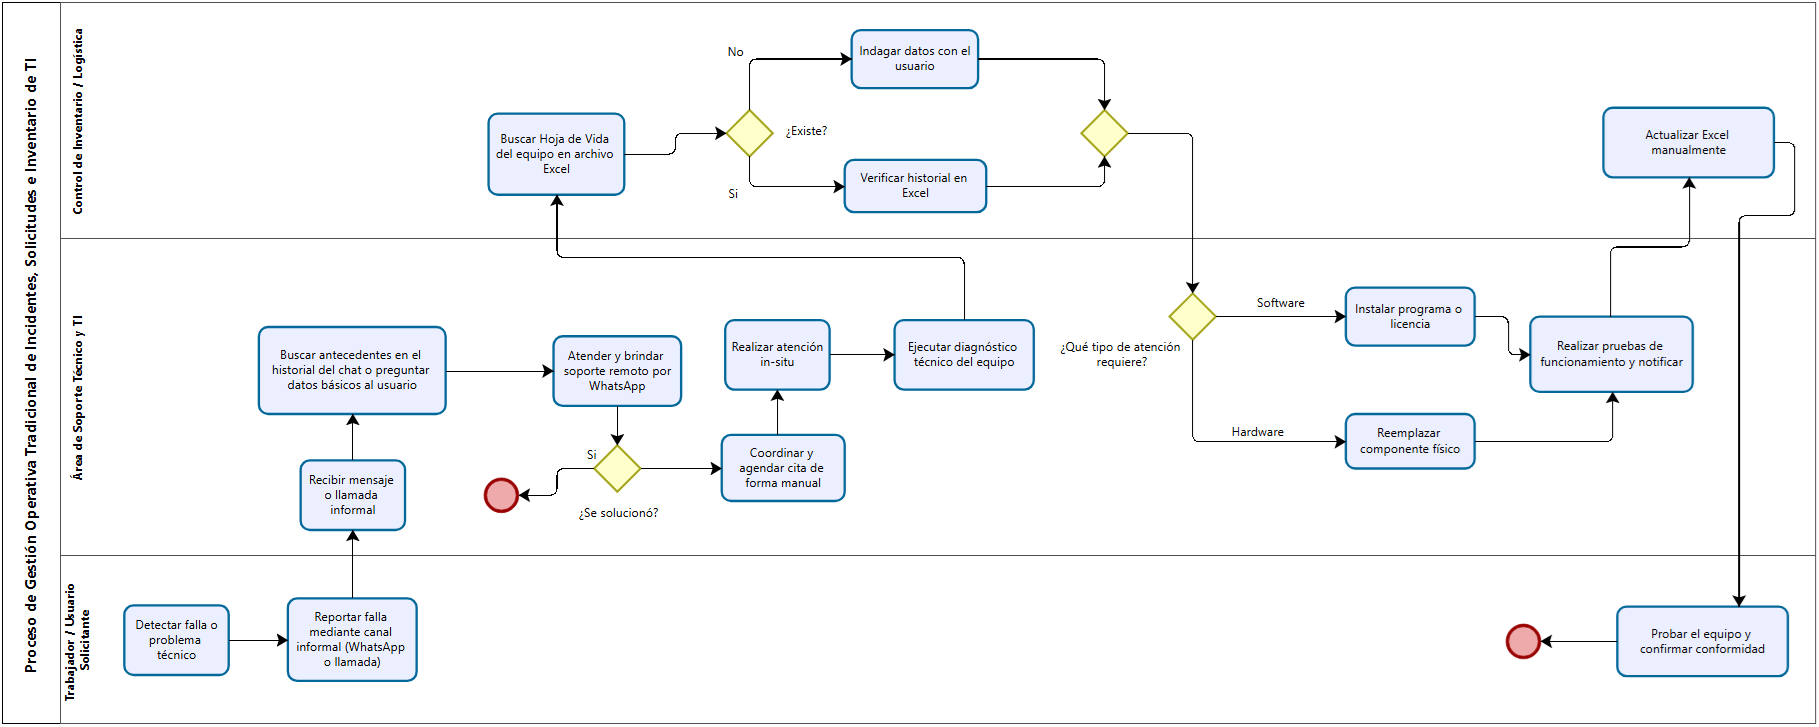
\includegraphics[width=\textwidth]{img/diagrama-proceso-sin-sistema.png}
    
    \vspace{0.4em}
    {\small \textit{Nota.} Representación BPMN del flujo manual de atención y control de inventario antes de la intervención del software.}
\end{figure}

\section{Efecto del Problema en el área del trabajo o en los resultados de la Empresa}

La ausencia de un sistema centralizado de gestión de atenciones técnicas e inventario informático en J\&P Periféricos S.A.C. genera efectos negativos directos que impactan tanto la productividad interna del Área de Soporte Técnico como la satisfacción final de los clientes corporativos.
Para evaluar el impacto de estos efectos en el área de trabajo, se resumen los principales indicadores afectados en la siguiente tabla.

\begingroup
\small
\renewcommand{\arraystretch}{1.15}
\begin{longtable}{@{} c p{13.8cm} @{}}
\caption{Identificación de las Causas del Problema Principal en el Área de Trabajo} \label{tab:causas_problema} \\
\hline
\textbf{N° KPI} & \textbf{IDENTIFICACIÓN DE LAS CAUSAS} \\
\hline
\endfirsthead

\multicolumn{2}{@{}l}{\textbf{Tabla \ref{tab:causas_problema}} \textit{(Continuación)}} \\[0.3em]
\hline
\textbf{N° KPI} & \textbf{IDENTIFICACIÓN DE LAS CAUSAS} \\
\hline
\endhead

\hline
\multicolumn{2}{r}{\textit{Continúa en la siguiente página\dots}} \\
\endfoot

\hline
\multicolumn{2}{@{}p{\textwidth}}{\small \textit{Nota.} Síntesis de las causas operativas identificadas en el diagnóstico del problema principal. Codificación idéntica a la encuesta de priorización (CA1–CA7).} \\
\endlastfoot

CA1 & Búsqueda manual de datos de equipos en archivos Excel desactualizados. \\
\hline
CA2 & Recepción y comunicación por canales informales (WhatsApp/llamadas) sin registro. \\
\hline
CA3 & Descoordinación y reubicación de horarios por cruces en visitas in-situ. \\
\hline
CA4 & Retraso en el escalamiento e identificación del historial de tickets previos. \\
\hline
CA5 & Verificación manual de términos y límites de servicio en contratos (SLA). \\
\hline
CA6 & Elaboración manual de reportes e informes de rendimiento de fin de mes. \\
\hline
CA7 & Carencia de indicadores de rendimiento (KPIs) para evaluar el tiempo de respuesta. \\
\end{longtable}
\endgroup

\section{Análisis de la causa raíz que genera el Problema}
Con la finalidad de identificar las causas fundamentales que originan la desorganización y la falta de trazabilidad en las atenciones técnicas de J\&P Periféricos S.A.C., se aplicó la técnica del Diagrama de Causa-Efecto (Diagrama de Ishikawa). 

\begin{figure}[H]
    \centering
    \captionsetup{justification=centering}
    \caption{Diagrama de Causa-Efecto (Ishikawa) del Problema Principal}
    \label{fig:diagrama_ishikawa}
    \vspace{0.4em}
    
    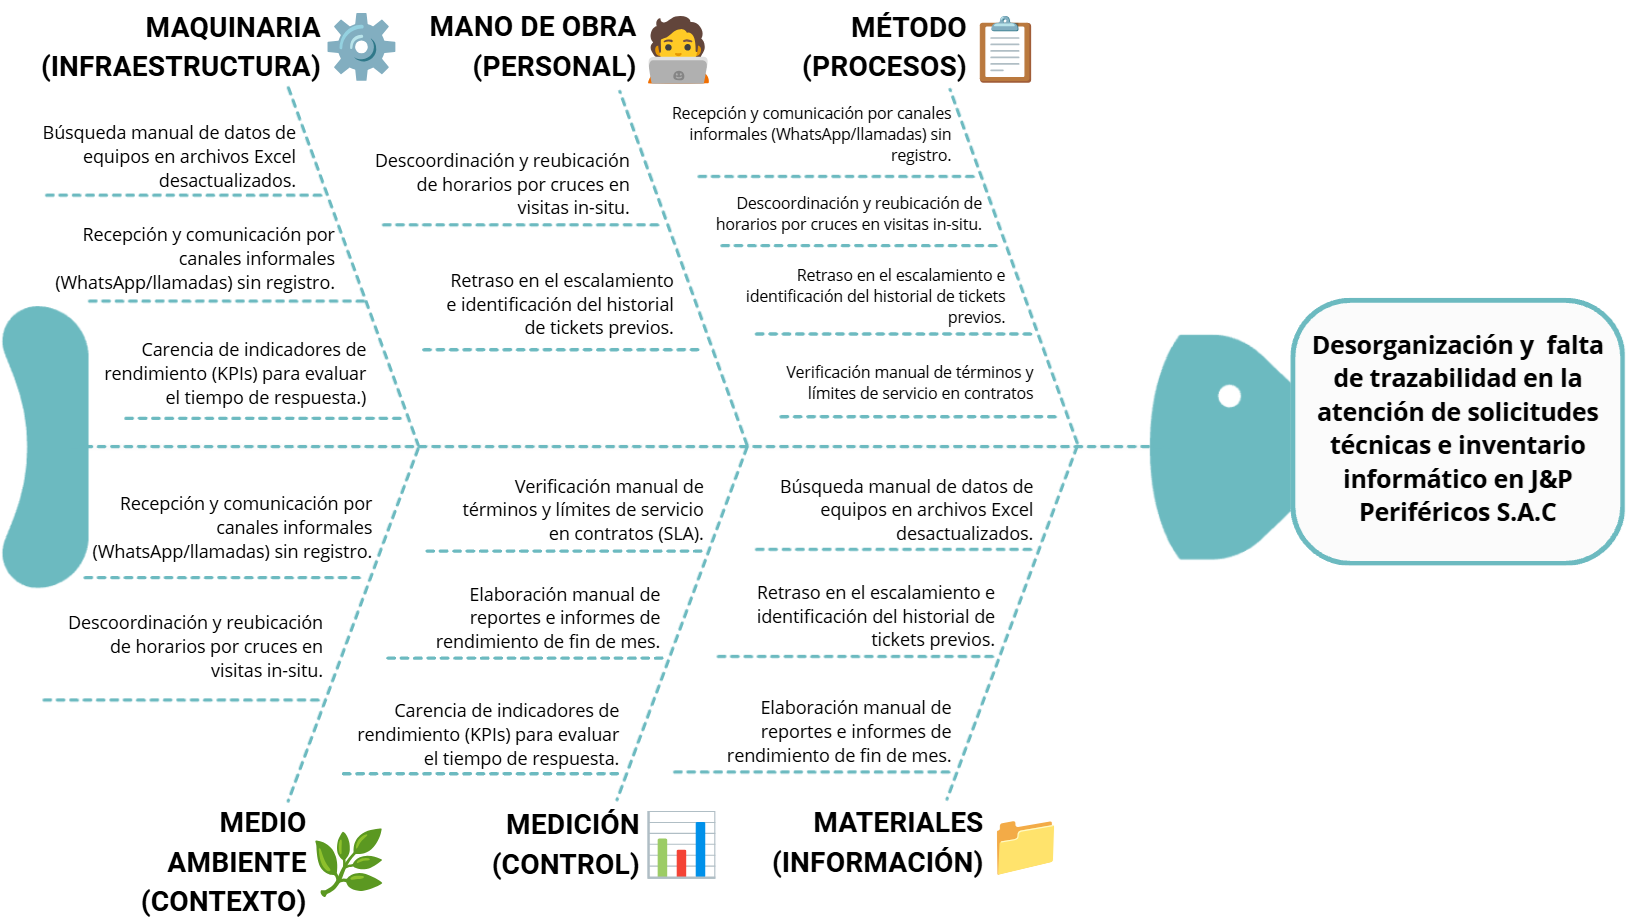
\includegraphics[width=1\textwidth]{img/diagrama_ishikawa.png}
    
    \vspace{0.4em}
    {\small \textit{Nota.} Representación gráfica de las causas raíz agrupadas por categorías de análisis.}
\end{figure}

La estructura de causa-efecto se organiza bajo las seis ramas clásicas del Diagrama de Ishikawa (6M), mapeando explícitamente los códigos CA1–CA7 de la Lista Maestra de Causas conforme al diagrama presentado:

\begin{itemize}[leftmargin=1.27cm]
    \item \textbf{Método (procesos):} CA2 (recepción y comunicación por canales informales sin registro), CA3 (programación empírica de visitas técnicas sin criterio unificado de agenda), CA4 (derivación y escalamiento de incidencias sin flujo estandarizado) y CA5 (verificación manual de términos y límites de servicio en contratos).
    \item \textbf{Mano de Obra (personal):} CA3 (descoordinación y reubicación de horarios por cruces en visitas \textit{in-situ}) y CA4 (retraso en el escalamiento e identificación del historial de tickets previos).
    \item \textbf{Maquinaria (infraestructura):} CA1 (búsqueda manual de datos de equipos en archivos Excel desactualizados), CA2 (falta de plataforma web centralizada para registrar y gestionar tickets) y CA7 (carencia de indicadores de rendimiento KPIs para evaluar el tiempo de respuesta).
    \item \textbf{Materiales (información):} CA1 (búsqueda manual de datos de equipos en archivos Excel desactualizados), CA4 (historial de tickets anteriores no centralizado para consulta rápida) y CA6 (elaboración manual de reportes e informes de rendimiento de fin de mes).
    \item \textbf{Medio Ambiente (contexto):} CA2 (atención fragmentada por mensajería y llamadas en el entorno de servicio) y CA3 (traslados y atención presencial en sedes de clientes sujetas a cambios).
    \item \textbf{Medición (control):} CA5 (verificación manual de términos y límites de servicio en contratos SLA), CA6 (elaboración manual de reportes e informes de rendimiento de fin de mes) y CA7 (carencia de indicadores de rendimiento KPIs para evaluar el tiempo de respuesta).
\end{itemize}

\vspace{0.4em}

\section{Priorización de causa Raíz}
\subsection{Lista de causas encuestadas}
Para evaluar la percepción del personal técnico y operativo respecto al impacto de cada causa raíz identificada, se aplicó un instrumento de encuesta evaluado mediante una escala Likert modificada (4: Muy Crítico / Muy Malo, 3: Crítico / Malo, 2: Regular / Leve, 1: Aceptable / Deficiente) sobre una población de 15 evaluadores.

\begingroup
\footnotesize
\renewcommand{\arraystretch}{1.1}
\begin{longtable}{@{} c p{9.6cm} *{4}{>{\centering\arraybackslash}p{0.6cm}} >{\centering\arraybackslash}p{1.2cm} @{}}
\caption{Resultados de la Encuesta de Valoración de Causas Raíz} \label{tab:encuesta_causas} \\
\hline
\textbf{N°} & \textbf{Identificación de las causas} & \textbf{4} & \textbf{3} & \textbf{2} & \textbf{1} & \textbf{Total Puntaje} \\
\hline
\endfirsthead

\multicolumn{7}{@{}l}{\textbf{Tabla \ref{tab:encuesta_causas}} \textit{(Continuación)}} \\[0.4em]
\hline
\textbf{N°} & \textbf{Identificación de las causas} & \textbf{4} & \textbf{3} & \textbf{2} & \textbf{1} & \textbf{Total Puntaje} \\
\hline
\endhead

\hline
\multicolumn{7}{r}{\textit{Continúa en la siguiente página\dots}} \\
\endfoot

\hline
\multicolumn{7}{@{}p{\textwidth}}{\small \textit{Nota.} Resultados consolidados de las encuestas aplicadas al personal de soporte técnico.} \\
\endlastfoot

CA1 & Búsqueda manual de datos de equipos en archivos Excel desactualizados. & 3 & 7 & 4 & 2 & 43 \\
\hline
CA2 & Recepción y comunicación por canales informales (WhatsApp/llamadas) sin registro. & 3 & 5 & 5 & 2 & 39 \\
\hline
CA3 & Descoordinación y reubicación de horarios por cruces en visitas in-situ. & 2 & 5 & 7 & 2 & 39 \\
\hline
CA4 & Retraso en el escalamiento e identificación del historial de tickets previos. & 2 & 8 & 2 & 1 & 37 \\
\hline
CA5 & Verificación manual de términos y límites de servicio en contratos (SLA). & 2 & 3 & 7 & 3 & 34 \\
\hline
CA6 & Elaboración manual de reportes e informes de rendimiento de fin de mes. & 1 & 3 & 6 & 4 & 29 \\
\hline
CA7 & Carencia de indicadores de rendimiento (KPIs) para evaluar el tiempo de respuesta. & 3 & 2 & 2 & 1 & 23 \\
\hline
\multicolumn{6}{r}{\textbf{Total General:}} & \textbf{244} \\
\end{longtable}
\endgroup

\subsection{Diagrama de Pareto en función al grado de las causas principales}
De acuerdo con la valoración obtenida en las encuestas, se procesaron los datos para construir la distribución acumulada bajo el principio de Pareto (80/20), identificando el grado de incidencia de las causas principales que generan la problemática en el área de soporte técnico de J\&P Periféricos S.A.C. Asimismo, se incluye el esquema de priorización de causa raíz que ilustra de manera directa el impacto de las variables críticas sobre el proceso operativo.

\begin{figure}[H]
    \centering
    \captionsetup{justification=centering}
    \caption{Diagrama de Pareto por Fenómenos}
    \label{fig:diagrama_pareto_por_fenomeno}
    \vspace{0.4em}
    
    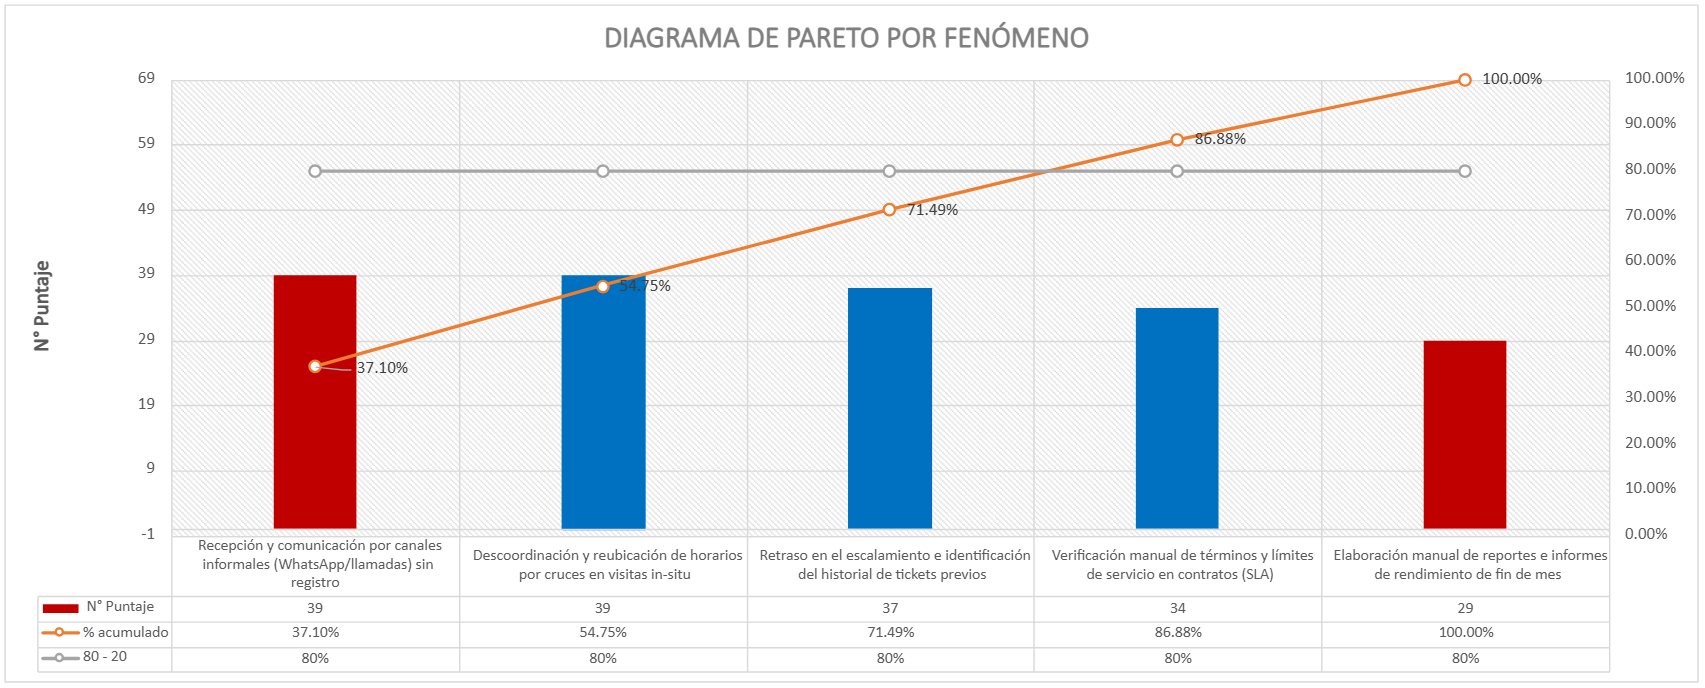
\includegraphics[width=0.95\textwidth]{img/diagrama_pareto_por_fenomeno.png}
    
    \vspace{0.4em}
    {\small \textit{Nota.} Representación gráfica de la distribución acumulada de causas encuestadas en el servicio de soporte técnico.}
\end{figure}

\begin{figure}[H]
    \centering
    \captionsetup{justification=centering}
    \caption{Diagrama de Priorizacion de Causa Raíz}
    \label{fig:diagrama_problema}
    \vspace{0.4em}
    
    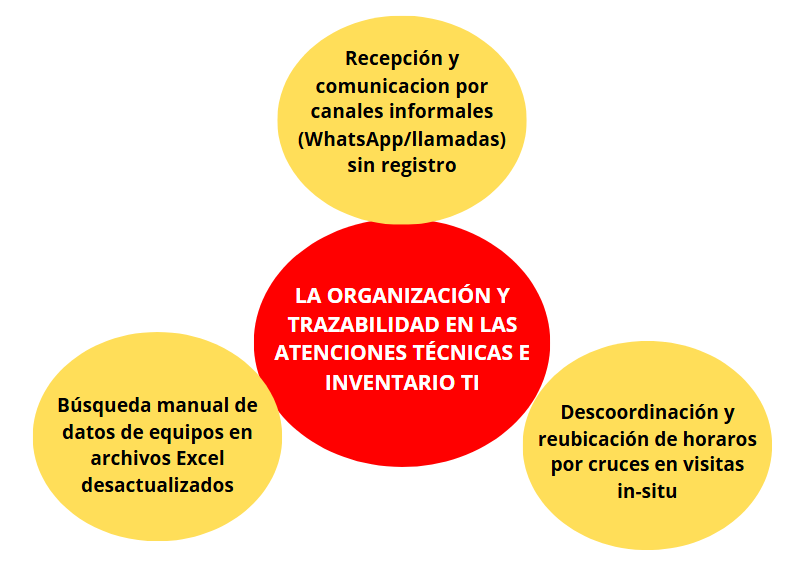
\includegraphics[width=0.95\textwidth]{img/diagrama_problema.png}
    
    \vspace{0.4em}
    {\small \textit{Nota.} Esquema de impacto directo de las causas priorizadas sobre la organizacion y trazabilidad.}
\end{figure}

\subsection{Análisis cualitativo y cuantitativo}

Para evaluar el impacto de cada causa raíz identificada en la encuesta de priorización (Tabla~\ref{tab:encuesta_causas}), se combina el análisis cualitativo del proceso con la cuantificación monetaria del tiempo improductivo operativo en el área de soporte técnico e \textit{in-situ} de J\&P Periféricos S.A.C. durante el período de mayo a septiembre de 2026 (395 atenciones totales y 3 técnicos operativos).

La pérdida económica asociada al tiempo improductivo se determina mediante la siguiente fórmula:

\begin{equation*}
\text{Pérdida Económica (S/)} = N_{\text{eventos}} \times \left(\frac{t_{\text{perdido (min)}}}{60}\right) \times C_{\text{H-H}}
\end{equation*}

donde $N_{\text{eventos}}$ corresponde al número de ocurrencias registradas o identificadas en el período, $t_{\text{perdido (min)}}$ es el tiempo promedio improductivo por ocurrencia expresado en minutos y $C_{\text{H-H}}$ es el costo operativo de hora-hombre del personal de soporte técnico e \textit{in-situ}, fijado internamente en S/ 12.00/hora.

Los datos empleados en el análisis provienen de la observación directa del flujo de atención, la revisión de los registros operativos disponibles (hojas de control, historial de tickets, contratos/SLA y reportes mensuales) y la estimación operativa en campo de los tiempos invertidos en actividades no productivas o repetitivas.

\subsubsection{Causa CA1: Búsqueda manual de datos de equipos en archivos Excel desactualizados}
\noindent \textit{Análisis cualitativo:} El inventario de activos TI y el historial de mantenimiento de los equipos de cómputo por cliente se administran mediante hojas de cálculo en Excel. Al no estar centralizada ni integrada con las solicitudes de atención, los técnicos deben realizar búsquedas manuales de especificaciones, garantías y mantenimientos previos antes o durante cada atención. Esto genera pérdida de tiempo operativo, errores en los diagnósticos y riesgo constante de trabajar con información obsoleta o duplicada. \\

\noindent \textit{Análisis cuantitativo:} 
A partir del registro de atenciones y la observación de búsqueda de activos, se identificaron 103 atenciones con demora por consulta manual en hojas de Excel (26\% del total). Con un tiempo perdido promedio de 25 minutos por incidencia y un costo de S/ 12.00 por hora-hombre (42.92 horas acumuladas), esta causa genera una pérdida económica de S/ 515.00 en el período de mayo a septiembre de 2026.

\begingroup
\small
\renewcommand{\arraystretch}{1.15}
\begin{longtable}{@{} p{4.2cm} >{\centering\arraybackslash}p{2.8cm} >{\centering\arraybackslash}p{2.8cm} >{\centering\arraybackslash}p{1.8cm} >{\centering\arraybackslash}p{2.2cm} @{}}
\caption{Análisis cuantitativo y económico por búsqueda manual de activos (Causa 1)} \label{tab:cuantitativo_causa1} \\
\hline
\textbf{Mes} & \textbf{Atenciones con demora} & \textbf{Total atenciones} & \textbf{Porcentaje} & \textbf{Pérdida estimada (S/)} \\
\hline
\endfirsthead

\multicolumn{5}{@{}l}{\textbf{Tabla \ref{tab:cuantitativo_causa1}} \textit{(Continuación)}} \\[0.4em]
\hline
\textbf{Mes} & \textbf{Atenciones con demora} & \textbf{Total atenciones} & \textbf{Porcentaje} & \textbf{Pérdida estimada (S/)} \\
\hline
\endhead

\hline
\multicolumn{5}{r}{\textit{Continúa en la siguiente página\dots}} \\
\endfoot

\hline
\multicolumn{5}{@{}p{\textwidth}}{\small \textit{Nota.} Registro mensual del impacto operativo y económico por la falta de inventario centralizado ($C_{\text{H-H}} = \text{S/ 12.00/h}$, 25 min por incidencia).} \\
\endlastfoot

May-26 & 18 & 70 & 26\% & S/ 90.00 \\
Jun-26 & 22 & 85 & 26\% & S/ 110.00 \\
Jul-26 & 26 & 95 & 27\% & S/ 130.00 \\
Aug-26 & 16 & 65 & 25\% & S/ 80.00 \\
Sep-26 & 21 & 80 & 26\% & S/ 105.00 \\
\hline
\textbf{Total} & \textbf{103} & \textbf{395} & \textbf{26\% (Prom.)} & \textbf{S/ 515.00} \\
\end{longtable}
\endgroup

\subsubsection{Causa CA2: Recepción y comunicación por canales informales (WhatsApp/llamadas) sin registro}
\noindent \textit{Análisis cualitativo:} La atención de incidentes mediante mensajes de WhatsApp y llamadas telefónicas directas impide registrar de forma oficial el requerimiento, provocando que las solicitudes queden traspapeladas o dispersas en los dispositivos móviles del personal. Esto genera confusión sobre qué técnico atendió a cada cliente, duplicidad en la comunicación y falta de seguimiento formal, ocasionando demoras considerables en el inicio de la atención y una constante pérdida de la trazabilidad operativa. \\

\noindent \textit{Análisis cuantitativo:} 
Mediante el seguimiento de solicitudes recibidas fuera de un canal formal entre mayo y septiembre de 2026, se registraron 149 solicitudes informales (38\% promedio del total de atenciones). Cada atención informal implica un tiempo improductivo promedio de 30 minutos por transcripción, repregunta y seguimiento disperso. Con un costo de S/ 12.00 por hora-hombre (74.50 horas acumuladas), se obtiene una pérdida económica de S/ 894.00 en el período analizado.

\begingroup
\small
\renewcommand{\arraystretch}{1.15}
\begin{longtable}{@{} p{4.2cm} >{\centering\arraybackslash}p{2.8cm} >{\centering\arraybackslash}p{2.8cm} >{\centering\arraybackslash}p{1.8cm} >{\centering\arraybackslash}p{2.2cm} @{}}
\caption{Análisis cuantitativo y económico de solicitudes por canales informales (Causa 2)} \label{tab:cuantitativo_causa2} \\
\hline
\textbf{Mes} & \textbf{Solicitudes informales} & \textbf{Total atenciones} & \textbf{Porcentaje} & \textbf{Pérdida estimada (S/)} \\
\hline
\endfirsthead

\multicolumn{5}{@{}l}{\textbf{Tabla \ref{tab:cuantitativo_causa2}} \textit{(Continuación)}} \\[0.4em]
\hline
\textbf{Mes} & \textbf{Solicitudes informales} & \textbf{Total atenciones} & \textbf{Porcentaje} & \textbf{Pérdida estimada (S/)} \\
\hline
\endhead

\hline
\multicolumn{5}{r}{\textit{Continúa en la siguiente página\dots}} \\
\endfoot

\hline
\multicolumn{5}{@{}p{\textwidth}}{\small \textit{Nota.} Consolidado mensual de incidencia e impacto económico por canales informales ($C_{\text{H-H}} = \text{S/ 12.00/h}$, 30 min por solicitud).} \\
\endlastfoot

May-26 & 26 & 70 & 37\% & S/ 156.00 \\
Jun-26 & 32 & 85 & 38\% & S/ 192.00 \\
Jul-26 & 37 & 95 & 39\% & S/ 222.00 \\
Aug-26 & 24 & 65 & 37\% & S/ 144.00 \\
Sep-26 & 30 & 80 & 38\% & S/ 180.00 \\
\hline
\textbf{Total} & \textbf{149} & \textbf{395} & \textbf{38\% (Prom.)} & \textbf{S/ 894.00} \\
\end{longtable}
\endgroup

\subsubsection{Causa CA3: Descoordinación y reubicación de horarios por cruces en visitas in-situ}
\noindent \textit{Análisis cualitativo:} La programación de visitas presenciales y soporte técnico in-situ en las sedes de los clientes se gestiona de manera manual y sin un calendario centralizado de disponibilidad técnica. Esto provoca cruces de agenda entre los técnicos asignados, reprogramaciones de última hora, tiempos muertos por traslados no optimizados y descoordinación con los horarios de atención de los clientes, lo que afecta la puntualidad y genera insatisfacción en el servicio. \\

\noindent \textit{Análisis cuantitativo:} 
A partir de la revisión de agendas y reprogramaciones de visitas presenciales, se registraron 81 visitas afectadas por cruces de horario (20\% promedio del total). Cada cruce genera un tiempo muerto promedio de 20 minutos de coordinación y reubicación. Valorizado a S/ 12.00 por hora-hombre (27.00 horas acumuladas), esta causa representa una pérdida económica de S/ 324.00 en el período evaluado.

\begingroup
\small
\renewcommand{\arraystretch}{1.15}
\begin{longtable}{@{} p{4.2cm} >{\centering\arraybackslash}p{2.8cm} >{\centering\arraybackslash}p{2.8cm} >{\centering\arraybackslash}p{1.8cm} >{\centering\arraybackslash}p{2.2cm} @{}}
\caption{Análisis cuantitativo y económico de visitas in-situ con reprogramación (Causa 3)} \label{tab:cuantitativo_causa3} \\
\hline
\textbf{Mes} & \textbf{Visitas con cruce de agenda} & \textbf{Total atenciones} & \textbf{Porcentaje} & \textbf{Pérdida estimada (S/)} \\
\hline
\endfirsthead

\multicolumn{5}{@{}l}{\textbf{Tabla \ref{tab:cuantitativo_causa3}} \textit{(Continuación)}} \\[0.4em]
\hline
\textbf{Mes} & \textbf{Visitas con cruce de agenda} & \textbf{Total atenciones} & \textbf{Porcentaje} & \textbf{Pérdida estimada (S/)} \\
\hline
\endhead

\hline
\multicolumn{5}{r}{\textit{Continúa en la siguiente página\dots}} \\
\endfoot

\hline
\multicolumn{5}{@{}p{\textwidth}}{\small \textit{Nota.} Distribución mensual de incidencias y pérdida económica por descoordinación en agenda presencial ($C_{\text{H-H}} = \text{S/ 12.00/h}$, 20 min por visita).} \\
\endlastfoot

May-26 & 14 & 70 & 20\% & S/ 56.00 \\
Jun-26 & 18 & 85 & 21\% & S/ 72.00 \\
Jul-26 & 21 & 95 & 22\% & S/ 84.00 \\
Aug-26 & 12 & 65 & 18\% & S/ 48.00 \\
Sep-26 & 16 & 80 & 20\% & S/ 64.00 \\
\hline
\textbf{Total} & \textbf{81} & \textbf{395} & \textbf{20\% (Prom.)} & \textbf{S/ 324.00} \\
\end{longtable}
\endgroup

\subsubsection{Causa CA4: Retraso en el escalamiento e identificación del historial de tickets previos}
\noindent \textit{Análisis cualitativo:} La falta de un flujo estandarizado para la asignación, seguimiento y escalamiento de tickets impide identificar el historial previo de cada incidencia, generando retrasos en la resolución y pérdida de trazabilidad operativa. Al no existir un registro centralizado de las atenciones anteriores, los técnicos deben re-diagnosticar casos ya atendidos, duplicando esfuerzos y prolongando los tiempos de resolución. \\

\noindent \textit{Análisis cuantitativo:}
Obtuvo un puntaje de 37 en la encuesta de priorización (Tabla~\ref{tab:encuesta_causas}), ubicándose en el cuarto lugar. Según la revisión de casos escalados o reabiertos y la observación del proceso de diagnóstico, se registran 95 casos en los cinco meses (entre 16 y 22 por mes) con un tiempo perdido promedio de 15 minutos por ticket (23.75 horas acumuladas), lo que equivale a una pérdida económica de S/ 285.00.

\begingroup
\small
\renewcommand{\arraystretch}{1.15}
\begin{longtable}{@{} p{4.2cm} >{\centering\arraybackslash}p{2.8cm} >{\centering\arraybackslash}p{2.4cm} >{\centering\arraybackslash}p{2.2cm} >{\centering\arraybackslash}p{2.2cm} @{}}
\caption{Análisis cuantitativo y económico por retraso en escalamiento e historial de tickets (Causa 4)} \label{tab:cuantitativo_causa4} \\
\hline
\textbf{Mes} & \textbf{Tickets afectados} & \textbf{Tiempo / caso (min)} & \textbf{Horas perdidas} & \textbf{Pérdida estimada (S/)} \\
\hline
\endfirsthead

\multicolumn{5}{@{}l}{\textbf{Tabla \ref{tab:cuantitativo_causa4}} \textit{(Continuación)}} \\[0.4em]
\hline
\textbf{Mes} & \textbf{Tickets afectados} & \textbf{Tiempo / caso (min)} & \textbf{Horas perdidas} & \textbf{Pérdida estimada (S/)} \\
\hline
\endhead

\hline
\multicolumn{5}{r}{\textit{Continúa en la siguiente página\dots}} \\
\endfoot

\hline
\multicolumn{5}{@{}p{\textwidth}}{\small \textit{Nota.} Impacto estimado a partir de la revisión de casos escalados/reabiertos y observación operativa ($C_{\text{H-H}} = \text{S/ 12.00/h}$).} \\
\endlastfoot

May-26 & 16 & 15 & 4.00 & S/ 48.00 \\
Jun-26 & 18 & 15 & 4.50 & S/ 54.00 \\
Jul-26 & 20 & 15 & 5.00 & S/ 60.00 \\
Aug-26 & 22 & 15 & 5.50 & S/ 66.00 \\
Sep-26 & 19 & 15 & 4.75 & S/ 57.00 \\
\hline
\textbf{Total} & \textbf{95} & \textbf{15 (Prom.)} & \textbf{23.75} & \textbf{S/ 285.00} \\
\end{longtable}
\endgroup

\subsubsection{Causa CA5: Verificación manual de términos y límites de servicio en contratos (SLA)}
\noindent \textit{Análisis cualitativo:} La verificación de la vigencia de los planes contratados, la cantidad máxima de equipos cubiertos y los tiempos máximos de atención comprometidos se realiza de forma manual y fragmentada, dificultando priorizar oportunamente las incidencias críticas y comprometiendo el cumplimiento de los Acuerdos de Nivel de Servicio (SLA). Esta carencia de control automatizado provoca que se brinde soporte a activos fuera de cobertura y afecte la formalidad del servicio. \\

\noindent \textit{Análisis cuantitativo:}
Obtuvo un puntaje de 34 en la encuesta de priorización (Tabla~\ref{tab:encuesta_causas}), ubicándose en el quinto lugar. A partir del contraste con los documentos de contratos/SLA y la observación de validación previa a la atención, se registran 93 verificaciones manuales en los cinco meses (entre 15 y 23 por mes) con un tiempo promedio de 12 minutos por revisión (18.60 horas acumuladas), generando una pérdida económica de S/ 223.20.

\begingroup
\small
\renewcommand{\arraystretch}{1.15}
\begin{longtable}{@{} p{4.2cm} >{\centering\arraybackslash}p{2.8cm} >{\centering\arraybackslash}p{2.4cm} >{\centering\arraybackslash}p{2.2cm} >{\centering\arraybackslash}p{2.2cm} @{}}
\caption{Análisis cuantitativo y económico por verificación manual de contratos y SLA (Causa 5)} \label{tab:cuantitativo_causa5} \\
\hline
\textbf{Mes} & \textbf{Revisiones SLA} & \textbf{Tiempo / caso (min)} & \textbf{Horas perdidas} & \textbf{Pérdida estimada (S/)} \\
\hline
\endfirsthead

\multicolumn{5}{@{}l}{\textbf{Tabla \ref{tab:cuantitativo_causa5}} \textit{(Continuación)}} \\[0.4em]
\hline
\textbf{Mes} & \textbf{Revisiones SLA} & \textbf{Tiempo / caso (min)} & \textbf{Horas perdidas} & \textbf{Pérdida estimada (S/)} \\
\hline
\endhead

\hline
\multicolumn{5}{r}{\textit{Continúa en la siguiente página\dots}} \\
\endfoot

\hline
\multicolumn{5}{@{}p{\textwidth}}{\small \textit{Nota.} Impacto estimado a partir de la revisión contractual y observación de validación de cobertura ($C_{\text{H-H}} = \text{S/ 12.00/h}$).} \\
\endlastfoot

May-26 & 15 & 12 & 3.00 & S/ 36.00 \\
Jun-26 & 17 & 12 & 3.40 & S/ 40.80 \\
Jul-26 & 20 & 12 & 4.00 & S/ 48.00 \\
Aug-26 & 23 & 12 & 4.60 & S/ 55.20 \\
Sep-26 & 18 & 12 & 3.60 & S/ 43.20 \\
\hline
\textbf{Total} & \textbf{93} & \textbf{12 (Prom.)} & \textbf{18.60} & \textbf{S/ 223.20} \\
\end{longtable}
\endgroup

\subsubsection{Causa CA6: Elaboración manual de reportes e informes de rendimiento de fin de mes}
\noindent \textit{Análisis cualitativo:} La elaboración manual de reportes e informes de rendimiento de fin de mes sobrecarga la operación del área técnica y limita la toma de decisiones basada en datos. Al no existir tableros analíticos automatizados, el personal técnico debe consolidar manualmente la información de atenciones, tiempos y cumplimiento de SLA, consumiendo tiempo que podría destinarse a la atención de incidencias. \\

\noindent \textit{Análisis cuantitativo:}
Obtuvo un puntaje de 29 en la encuesta de priorización (Tabla~\ref{tab:encuesta_causas}), ubicándose en el sexto lugar. Según la revisión de informes mensuales emitidos y la observación del cierre operativo, se elabora 1 reporte consolidado mensual con una dedicación promedio de 4.00 horas por cierre (20.00 horas en cinco meses), lo que representa una pérdida económica de S/ 240.00.

\begingroup
\small
\renewcommand{\arraystretch}{1.15}
\begin{longtable}{@{} p{4.2cm} >{\centering\arraybackslash}p{2.6cm} >{\centering\arraybackslash}p{2.6cm} >{\centering\arraybackslash}p{2.2cm} >{\centering\arraybackslash}p{2.2cm} @{}}
\caption{Análisis cuantitativo y económico por elaboración manual de reportes mensuales (Causa 6)} \label{tab:cuantitativo_causa6} \\
\hline
\textbf{Mes} & \textbf{Reportes emitidos} & \textbf{Horas de cierre} & \textbf{Costo H-H (S/)} & \textbf{Pérdida estimada (S/)} \\
\hline
\endfirsthead

\multicolumn{5}{@{}l}{\textbf{Tabla \ref{tab:cuantitativo_causa6}} \textit{(Continuación)}} \\[0.4em]
\hline
\textbf{Mes} & \textbf{Reportes emitidos} & \textbf{Horas de cierre} & \textbf{Costo H-H (S/)} & \textbf{Pérdida estimada (S/)} \\
\hline
\endhead

\hline
\multicolumn{5}{r}{\textit{Continúa en la siguiente página\dots}} \\
\endfoot

\hline
\multicolumn{5}{@{}p{\textwidth}}{\small \textit{Nota.} Impacto estimado a partir de los informes mensuales elaborados y el tiempo de consolidación de datos.} \\
\endlastfoot

May-26 & 1 & 4.00 & S/ 12.00 & S/ 48.00 \\
Jun-26 & 1 & 4.00 & S/ 12.00 & S/ 48.00 \\
Jul-26 & 1 & 4.00 & S/ 12.00 & S/ 48.00 \\
Aug-26 & 1 & 4.00 & S/ 12.00 & S/ 48.00 \\
Sep-26 & 1 & 4.00 & S/ 12.00 & S/ 48.00 \\
\hline
\textbf{Total} & \textbf{5} & \textbf{20.00} & \textbf{S/ 12.00} & \textbf{S/ 240.00} \\
\end{longtable}
\endgroup

\subsubsection{Causa CA7: Carencia de indicadores de rendimiento (KPIs) para evaluar el tiempo de respuesta}
\noindent \textit{Análisis cualitativo:} La falta de un sistema con backend robusto y modular que centralice las reglas de negocio impide la monitorización en tiempo real de los indicadores de rendimiento y la validación automatizada de contratos, sobrecargando la operación y comprometiendo la calidad del servicio técnico. Sin KPIs como MTTA, MTTR, FCR y CSAT, la gerencia no puede evaluar objetivamente el desempeño del equipo técnico ni el cumplimiento de los SLA. \\

\noindent \textit{Análisis cuantitativo:}
Obtuvo un puntaje de 23 en la encuesta de priorización (Tabla~\ref{tab:encuesta_causas}), ubicándose en el séptimo lugar. A partir de la observación de las actividades de control y seguimiento de tiempos del área, se registra 1 revisión mensual dedicada al control manual de indicadores/tiempos con 2.00 horas por mes (10.00 horas en cinco meses), sin duplicar los tiempos ya contabilizados en las demás causas, lo que equivale a una pérdida económica de S/ 120.00.

\begingroup
\small
\renewcommand{\arraystretch}{1.15}
\begin{longtable}{@{} p{4.2cm} >{\centering\arraybackslash}p{2.6cm} >{\centering\arraybackslash}p{2.6cm} >{\centering\arraybackslash}p{2.2cm} >{\centering\arraybackslash}p{2.2cm} @{}}
\caption{Análisis cuantitativo y económico por carencia de indicadores KPI (Causa 7)} \label{tab:cuantitativo_causa7} \\
\hline
\textbf{Mes} & \textbf{Revisiones / mes} & \textbf{Horas de control} & \textbf{Costo H-H (S/)} & \textbf{Pérdida estimada (S/)} \\
\hline
\endfirsthead

\multicolumn{5}{@{}l}{\textbf{Tabla \ref{tab:cuantitativo_causa7}} \textit{(Continuación)}} \\[0.4em]
\hline
\textbf{Mes} & \textbf{Revisiones / mes} & \textbf{Horas de control} & \textbf{Costo H-H (S/)} & \textbf{Pérdida estimada (S/)} \\
\hline
\endhead

\hline
\multicolumn{5}{r}{\textit{Continúa en la siguiente página\dots}} \\
\endfoot

\hline
\multicolumn{5}{@{}p{\textwidth}}{\small \textit{Nota.} Impacto estimado a partir de la observación de control de tiempos sin duplicar tiempos de otras causas.} \\
\endlastfoot

May-26 & 1 & 2.00 & S/ 12.00 & S/ 24.00 \\
Jun-26 & 1 & 2.00 & S/ 12.00 & S/ 24.00 \\
Jul-26 & 1 & 2.00 & S/ 12.00 & S/ 24.00 \\
Aug-26 & 1 & 2.00 & S/ 12.00 & S/ 24.00 \\
Sep-26 & 1 & 2.00 & S/ 12.00 & S/ 24.00 \\
\hline
\textbf{Total} & \textbf{5} & \textbf{10.00} & \textbf{S/ 12.00} & \textbf{S/ 120.00} \\
\end{longtable}
\endgroup

Con el propósito de cuantificar el impacto financiero que generan las deficiencias operativas detectadas en la gestión de soporte técnico e inventario de TI, se realizó una valorización del tiempo improductivo asociado a cada causa raíz durante el periodo comprendido entre mayo y septiembre de 2026. Para este cálculo se tomó como base un costo hora-hombre de S/ 12.00, permitiendo traducir las horas perdidas en montos acumulados y promedios mensuales concretos. En la \hyperref[tab:consolidado_perdidas_cap3]{Tabla~\ref*{tab:consolidado_perdidas_cap3}} se presenta el consolidado detallado de estas pérdidas económicas desagregadas por cada uno de los siete problemas identificados.

\begingroup
\small
\renewcommand{\arraystretch}{1.15}
\begin{longtable}{@{} c p{8.8cm} >{\centering\arraybackslash}p{2.4cm} >{\centering\arraybackslash}p{2.4cm} @{}}
\caption{Consolidado de pérdidas económicas por causa raíz (mayo – septiembre 2026)} \label{tab:consolidado_perdidas_cap3} \\
\hline
\textbf{Código} & \textbf{Causa raíz} & \textbf{Pérdida 5 meses (S/)} & \textbf{Promedio mensual (S/)} \\
\hline
\endfirsthead

\multicolumn{4}{@{}l}{\textbf{Tabla \ref{tab:consolidado_perdidas_cap3}} \textit{(Continuación)}} \\[0.4em]
\hline
\textbf{Código} & \textbf{Causa raíz} & \textbf{Pérdida 5 meses (S/)} & \textbf{Promedio mensual (S/)} \\
\hline
\endhead

\hline
\multicolumn{4}{r}{\textit{Continúa en la siguiente página\dots}} \\
\endfoot

\hline
\multicolumn{4}{@{}p{\textwidth}}{\small \textit{Nota.} Resumen de pérdidas por tiempo improductivo operativo calculadas con $C_{\text{H-H}} = \text{S/ 12.00/hora}$.} \\
\endlastfoot

CA1 & Búsqueda manual de datos de equipos en archivos Excel desactualizados & S/ 515.00 & S/ 103.00 \\
\hline
CA2 & Recepción y comunicación por canales informales (WhatsApp/llamadas) sin registro & S/ 894.00 & S/ 178.80 \\
\hline
CA3 & Descoordinación y reubicación de horarios por cruces en visitas in-situ & S/ 324.00 & S/ 64.80 \\
\hline
CA4 & Retraso en el escalamiento e identificación del historial de tickets previos & S/ 285.00 & S/ 57.00 \\
\hline
CA5 & Verificación manual de términos y límites de servicio en contratos (SLA) & S/ 223.20 & S/ 44.64 \\
\hline
CA6 & Elaboración manual de reportes e informes de rendimiento de fin de mes & S/ 240.00 & S/ 48.00 \\
\hline
CA7 & Carencia de indicadores de rendimiento (KPIs) para evaluar el tiempo de respuesta & S/ 120.00 & S/ 24.00 \\
\hline
\multicolumn{2}{r}{\textbf{Total General:}} & \textbf{S/ 2 601.20} & \textbf{S/ 520.24} \\
\end{longtable}
\endgroup
\cleardoublepage

\chapter[CAPÍTULO IV]{PROPUESTA TÉCNICA DE LA MEJORA}

\section{Plan de Acción de la Mejora Propuesta}

Este capítulo presenta la estrategia de implementación del sistema web help-desk y control de activos TI, formalizada en el \hyperlink{anexo4_acta}{Anexo 4} (\textit{Acta de Constitución del Proyecto}). Para ejecutar la mejora de forma ordenada, el plan se organiza bajo dos enfoques complementarios:

\begin{itemize}
    \item \textbf{Gestión y desarrollo (\textit{Scrumban}):} Combina \textbf{Scrum} para las entregas incrementales por \textit{sprints} y \textbf{Kanban} para el control visual del flujo y límites \textit{WIP} (\textit{Frontend} en Next.js; \textit{Backend} en NestJS con Prisma ORM y MySQL).
    \item \textbf{Analítica y métricas (CRISP-DM):} Estructura el procesamiento del historial de incidencias, activos y auditoría para alimentar los tableros y KPIs gerenciales.
\end{itemize}

A continuación se detallan las metodologías, requerimientos y fases de ejecución del plan.

\subsection{Metodología Scrum}
La metodología \textbf{Scrum} permite gestionar el ciclo de vida del desarrollo del software mediante iteraciones cortas denominadas \textit{sprints}.
\begin{itemize}
\item \textbf{Aplicación en el proyecto:} Se aplica en la planificación y entrega incremental de los módulos del sistema (Módulo de Autenticación y Usuarios, Gestión de Clientes y Sucursales, Gestión de Tickets, Control de Equipos/Hardware o Software, y el motor de Citas).
\item \textbf{Impacto operativo:} Facilita la adaptación continua a los requerimientos prioritarios del negocio mediante la gestión del \textit{Product Backlog} y \textit{Sprint Backlog}, asegurando entregas funcionales probadas al final de cada ciclo de desarrollo.
\end{itemize}

\begin{table}[H]
\centering
\small
\renewcommand{\arraystretch}{1.2}
\caption{Conformación del Equipo Scrum del Proyecto}
\label{tab:equipo_scrum}
\begin{tabular}{@{} p{3.5cm} p{4.5cm} p{6.5cm} @{}}
\toprule
\textbf{Rol Scrum} & \textbf{Integrante} & \textbf{Responsabilidad Principal} \\
\midrule
Product Owner & Julio Flores Vicuña & Define y prioriza los requerimientos del negocio y el \textit{Product Backlog}. \\
Scrum Master / Developer & Jack Daniel Leandro Hernández & Facilita el marco Scrum, remueve impedimentos y participa activamente en la arquitectura y desarrollo de software. \\
Developer & Giovanni Denis Jara Hilario & Participa en el diseño, desarrollo y entregas incrementales del sistema. \\
Developer & Alvaro Jesus Solis Rivadeneyra & Participa en el diseño, desarrollo y entregas incrementales del sistema. \\
\bottomrule
\end{tabular}
\\[0.3em]
{\small \textit{Nota.} Elaboración propia a partir de la organización del equipo de trabajo.}
\end{table}

\subsection{Metodología Kanban}
Implementada para el control visual del flujo operativo de atención de tickets y tareas diarias tanto en la fase de desarrollo como en la operación continua del sistema.
\begin{itemize}
\item \textbf{Aplicación en el proyecto:} En el tablero operativo interactivo donde los analistas de soporte visualizan el ciclo de vida de los tickets (desde que ingresan como \textit{Pendiente}, pasan a \textit{Asignado}, \textit{En Progreso}, \textit{Derivado InSitu}, hasta su \textit{Cierre} o paso a \textit{En Espera Repuesto}).
\item \textbf{Impacto operativo:} Permite limitar el trabajo en curso (\textit{WIP - Work in Progress}), identificar cuellos de botella en tiempo real y transparentar el estado de avance de las atenciones técnicas.
\end{itemize}

\subsection{Metodología CRISP-DM}
Aplicada para estructurar el análisis, procesamiento y minería de los datos generados por la plataforma.
\begin{itemize}
\item \textbf{Aplicación en el proyecto:} En el diseño y estructuración del módulo de \textbf{Dashboard y KPIs}, procesando los datos relacionales de MySQL y los registros en formato JSON de la tabla \texttt{auditoria\_eventos} de la base de datos.
\item \textbf{Impacto operativo:} Garantiza un flujo estructurado en 6 fases (Comprensión del negocio, Comprensión de los datos, Preparación de datos, Modelado, Evaluación y Despliegue) para transformar el historial de incidencias y la carga laboral de los técnicos en métricas de rendimiento precisas para la gerencia.
\end{itemize}

\subsection{Requerimientos del Sistema}
Para el correcto funcionamiento del sistema web help-desk, se han definido y clasificado los requerimientos funcionales y no funcionales que guiarán el desarrollo de la arquitectura y la base de datos.

\subsubsection{Requerimientos Funcionales}
Los requerimientos funcionales especifican las operaciones, interacciones y reglas de negocio que el software debe ejecutar de manera obligatoria para satisfacer las necesidades de los usuarios (administradores, personal técnico y clientes), cuyo detalle operativo se presenta en la Tabla \ref{tab:req_funcionales}.

\begingroup
\footnotesize
\renewcommand{\arraystretch}{1.2}
\begin{longtable}{@{} p{1.8cm} p{3.2cm} p{7.0cm} p{3.2cm} @{}}
\caption{{Requerimientos Funcionales del Sistema}} \label{tab:req_funcionales} \\
\toprule
\textbf{Cod. Req.} & \textbf{Nombre} & \textbf{Descripción} & \textbf{Rol} \\
\midrule
\endfirsthead

\multicolumn{4}{@{}l}{\textbf{Tabla \ref{tab:req_funcionales}} \textit{(Continuación)}} \\[0.4em]
\toprule
\textbf{Cod. Req.} & \textbf{Nombre} & \textbf{Descripción} & \textbf{Rol} \\
\midrule
\endhead

\midrule
\multicolumn{4}{r}{\textit{Continúa en la siguiente página\dots}} \\
\endfoot

\bottomrule
\multicolumn{4}{@{}p{\textwidth}}{\small \textit{Nota.} Detalle completo de los requerimientos funcionales del sistema web help-desk.} \\
\endlastfoot

RF-001 & Gestión de Usuarios y Autenticación & Registro, inicio de sesión con tokens JWT sin estado, cifrado Bcrypt, roles y control de sesiones concurrentes (\textit{soft\_locks}). & ADMIN, SOPORTE, CLIENTE \\
RF-002 & Gestión Organizativa y Planes & Registro y administración de clientes vinculados a un plan de soporte (costo, vigencia y límite de equipos). & ADMINISTRADOR \\
RF-003 & Gestión de Sucursales y Áreas & Administración de sedes físicas y departamentos operativos internos para la ubicación de activos y personal. & ADMIN, CLIENTE \\
RF-004 & Cobertura Geográfica de Técnicos & Asociación mediante tabla pivote (\texttt{tecnicos\_zonas}) de técnicos de campo autorizados por zona geográfica. & ADMINISTRADOR \\
RF-005 & Ciclo de Vida de Tickets & Reporte de incidencias vinculadas a equipos con generación de PIN y gestión de su máquina de estados. & CLIENTE, SOPORTE \\
RF-006 & Parque Informático de Equipos & Registro de equipos de cómputo (Desktop, Laptop) con estado operativo y vinculación al responsable. & ADMIN, SOPORTE \\
RF-007 & Inventario de Hardware & Gestión maestro de componentes físicos, repuestos y su hoja de vida histórica (\texttt{registro\_hardware}). & ADMIN, SOPORTE \\
RF-008 & Gestión de Software y Licencias & Control de catálogo global de software, licencias, claves maestras y acoplamiento por endpoint. & ADMIN, SOPORTE \\
RF-009 & Agendamiento de Visitas In-Situ & Programación de citas de soporte presencial vinculando ticket, técnico, sucursal y control anti-cruces. & SOPORTE \\
RF-010 & Auditoría de Eventos Críticos & Registro histórico detallado de cambios sobre tickets y citas utilizando metadatos estructurados JSON. & ADMINISTRADOR \\
RF-011 & Dashboards e Indicadores & Generación de reportes analíticos de volumen de tickets, tiempos de atención y cumplimiento de SLA. & ADMIN, SOPORTE \\
\end{longtable}
\endgroup

\subsubsection{Requerimientos No Funcionales}
Los requerimientos no funcionales definen los atributos de calidad del sistema, tales como rendimiento, seguridad, disponibilidad, escalabilidad y compatibilidad técnica con los entornos de ejecución, los cuales se consolidan en la Tabla \ref{tab:req_nofuncionales}.

\begingroup
\footnotesize
\renewcommand{\arraystretch}{1.2}
\begin{longtable}{@{} p{1.8cm} p{3.2cm} p{7.0cm} p{3.2cm} @{}}
\caption{{Requerimientos No Funcionales del Sistema}} \label{tab:req_nofuncionales} \\
\toprule
\textbf{Cod. Req.} & \textbf{Nombre} & \textbf{Descripción} & \textbf{Rol} \\
\midrule
\endfirsthead

\multicolumn{4}{@{}l}{\textbf{Tabla \ref{tab:req_nofuncionales}} \textit{(Continuación)}} \\[0.4em]
\toprule
\textbf{Cod. Req.} & \textbf{Nombre} & \textbf{Descripción} & \textbf{Rol} \\
\midrule
\endhead

\midrule
\multicolumn{4}{r}{\textit{Continúa en la siguiente página\dots}} \\
\endfoot

\bottomrule
\multicolumn{4}{@{}p{\textwidth}}{\small \textit{Nota.} Especificaciones de calidad y rendimiento técnico del sistema.} \\
\endlastfoot

RNF-001 & Comunicación en Tiempo Real & Transmisión bidireccional y de baja latencia para notificaciones y estados de tickets mediante WebSockets. & Todos los roles \\
RNF-002 & Seguridad e Integridad & Autenticación segura mediante JWT sin estado, Bcrypt y control de acceso basado en roles (RBAC). & Todos los roles \\
RNF-003 & Persistencia y Escalabilidad & Uso de base de datos relacional MySQL con Prisma ORM y soporte para metadatos JSON dinámicos. & ADMIN, SOPORTE \\
RNF-004 & Rendimiento en Búsquedas & Procesamiento de consultas masivas de inventario y reportes de dashboard en menos de 3 segundos. & ADMIN, SOPORTE \\
RNF-005 & Disponibilidad y Concurrencia & Garantizar 99.8\% de disponibilidad para acceso simultáneo apoyado en bloqueos temporales (\textit{soft\_locks}). & Todos los roles \\
RNF-006 & Arquitectura Limpia & Backend estructurado en NestJS bajo Arquitectura Hexagonal y principios SOLID para alta mantenibilidad. & ADMIN, SOPORTE \\
RNF-007 & Trazabilidad y Auditoría & Registro automatizado de eventos críticos e historiales en tablas de auditoría y hojas de vida. & ADMIN, SOPORTE \\
RNF-008 & Compatibilidad Responsive & Interfaz frontend adaptable a distintos dispositivos y navegadores web modernos (Chrome, Edge, Firefox). & Todos los roles \\
\end{longtable}
\endgroup

\subsection{Fases del Plan de Acción por Sprints}
El desarrollo e implementación de la mejora en J\&P Periféricos S.A.C. se estructura cronológicamente en iteraciones cortas agrupadas en fases técnicas, permitiendo asegurar entregas incrementales y controladas de la solución.

\subsubsection{Fase 1: Análisis y Modelado (Sprints 0 - 1)}
Esta fase inicial comprende la recopilación de especificaciones, el diseño conceptual de la arquitectura de datos, el modelado de procesos y la definición formal de los diagramas UML, cuyas actividades y plazos se detallan en la Tabla \ref{tab:fase1}.

\begingroup
\small
\renewcommand{\arraystretch}{1.25}
\begin{longtable}{@{} p{3.2cm} p{8.8cm} p{3.0cm} @{}}
\caption{{Fase 1: Análisis y Modelado (Sprints 0 - 1)}} \label{tab:fase1} \\
\toprule
\textbf{Actividad / Tarea} & \textbf{Descripción del Entregable} & \textbf{Duración / Plazo} \\
\midrule
\endfirsthead

\multicolumn{3}{@{}l}{\textbf{Tabla \ref{tab:fase1}} \textit{(Continuación)}} \\[0.4em]
\toprule
\textbf{Actividad / Tarea} & \textbf{Descripción del Entregable} & \textbf{Duración / Plazo} \\
\midrule
\endhead

\midrule
\multicolumn{3}{r}{\textit{Continúa en la siguiente página\dots}} \\
\endfoot

\bottomrule
\multicolumn{3}{@{}p{\textwidth}}{\small \textit{Nota.} Cronograma y entregables detallados para la fase de análisis y modelado.} \\
\endlastfoot

TR00 - Planificación y gestión del proyecto & Planificación, ceremonias de sprint, revisiones y documentación transversal. & 14 días \\
TR01 - Alcance y Problemática & Definición del alcance del proyecto y problemática de trazabilidad TI. & 4 días \\
TR02 - Modelado de Negocio & Modelado del flujo de negocio y matriz de permisos por rol. & 5 días \\
TR03 - Requisitos & Redacción de especificación de Requisitos Funcionales y No Funcionales. & 5 días \\
TR04 - EDT / WBS & Construcción de la Estructura Desglosada de Trabajo y línea base. & 4 días \\
TR05 - Análisis Hoja de Vida & Análisis de requerimientos para el módulo de Hoja de Vida de Equipos. & 4 días \\
TR06 - Matriz CRUD & Elaboración de matriz CRUD de accesos y permisos por rol. & 4 días \\
TR07 - Diagramas UML & Diseño de diagramas UML y especificaciones de Casos de Uso. & 6 días \\
TR08 - Esquema Relacional & Creación del esquema relacional y enums en \texttt{schema.prisma}. & 4 días \\
\textbf{Total Fase 1} & & \textbf{50 días} \\
\end{longtable}
\endgroup

Como evidencia del cumplimiento de esta fase inicial, a continuación se presentan los tableros de gestión, los gráficos de seguimiento (\textit{burndown charts}) y el diseño del esquema de base de datos (tarea TR08):

\begin{figure}[H]
\centering
\captionsetup{justification=centering}
\caption{Tablero de Jira - Sprint 0 }
\label{fig:evidencia_sprint_0}
\vspace{0.2em}
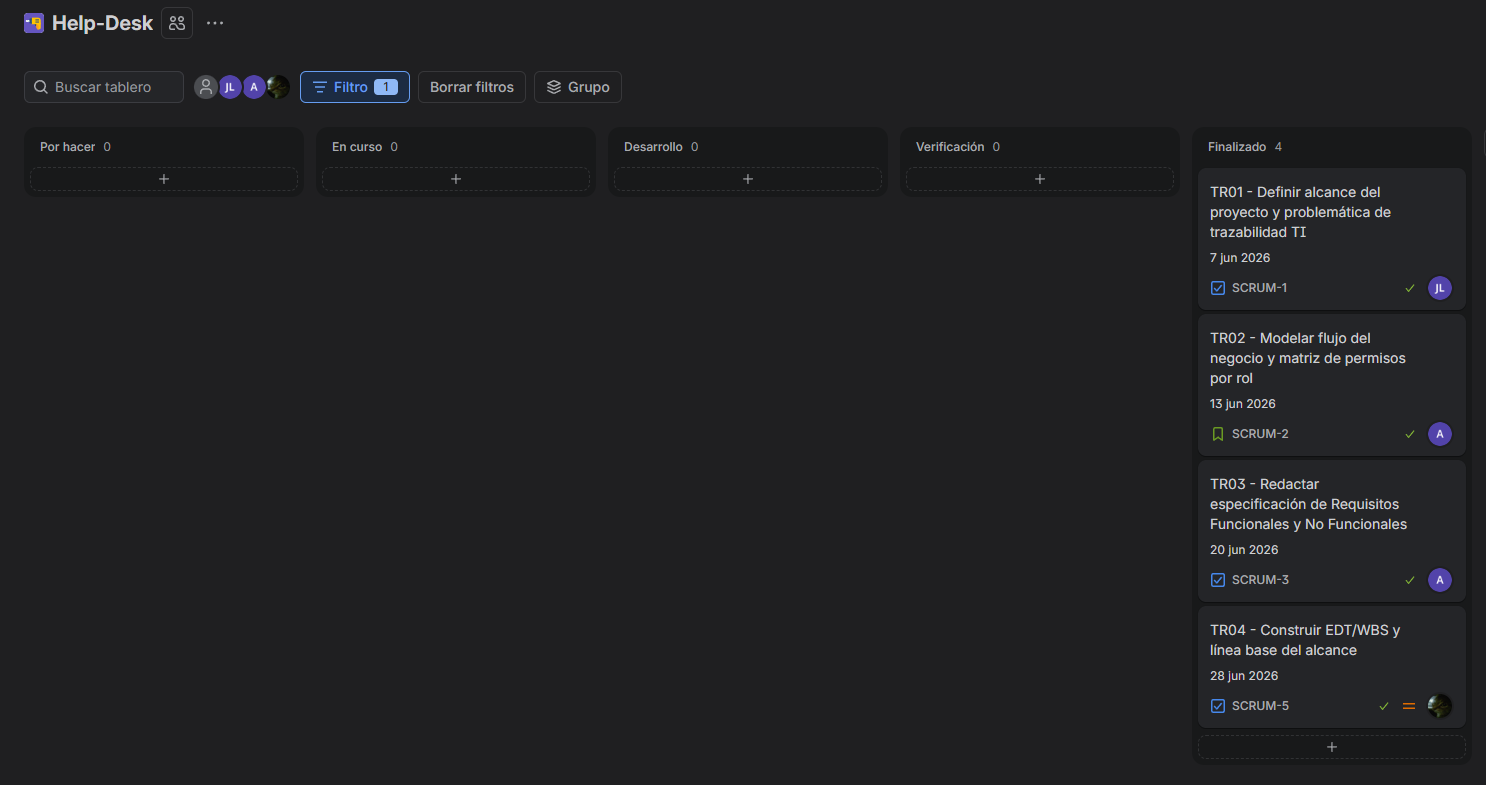
\includegraphics[width=0.92\textwidth]{tablero_sprint_0.png}
\\[0.2em]
{\small \textit{Nota.} Vista general del tablero de tareas correspondiente al análisis, modelado de negocio y arquitectura base}
\end{figure}

\begin{figure}[H]
\centering
\captionsetup{justification=centering}
\caption{Burndown Chart - Sprint 0}
\label{fig:burndown_sprint_0}
\vspace{0.2em}
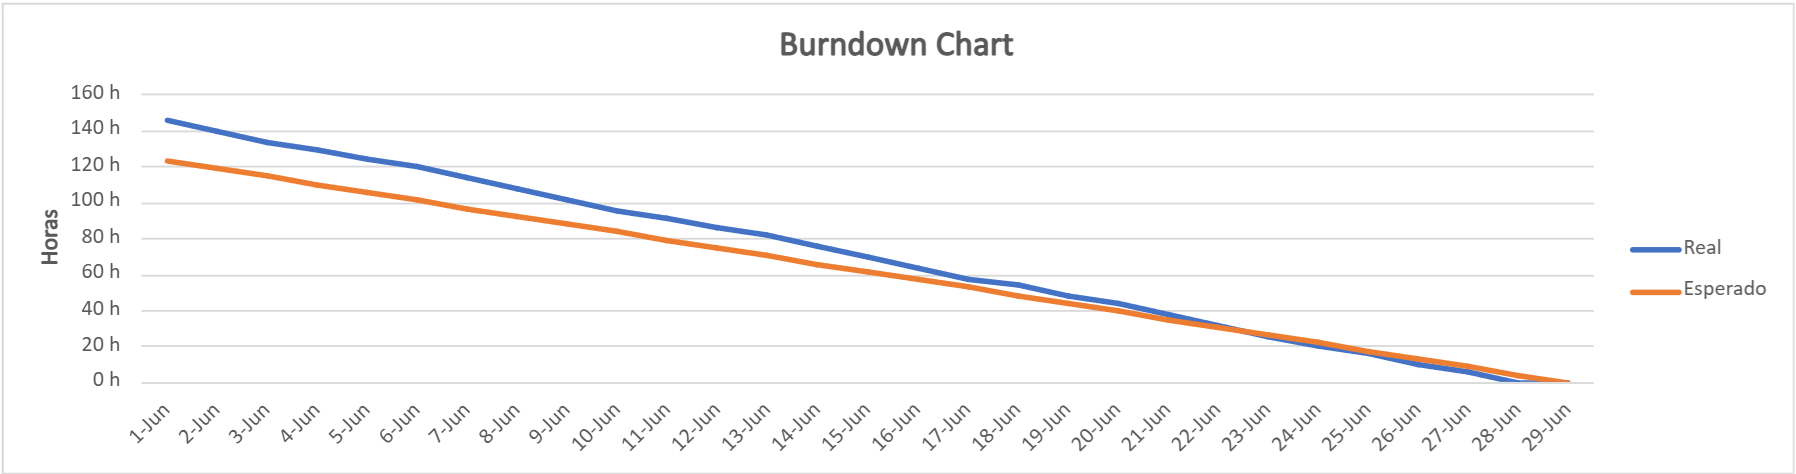
\includegraphics[width=0.92\textwidth]{burdowchart_sprint0.png}
\\[0.2em]
{\small \textit{Nota.} Elaboración propia. Seguimiento de horas estimadas frente al avance real durante el Sprint 0.}
\end{figure}

\begin{figure}[H]
\centering
\captionsetup{justification=centering}
\caption{Tablero de Jira - Sprint 1}
\label{fig:evidencia_sprint_1}
\vspace{0.2em}
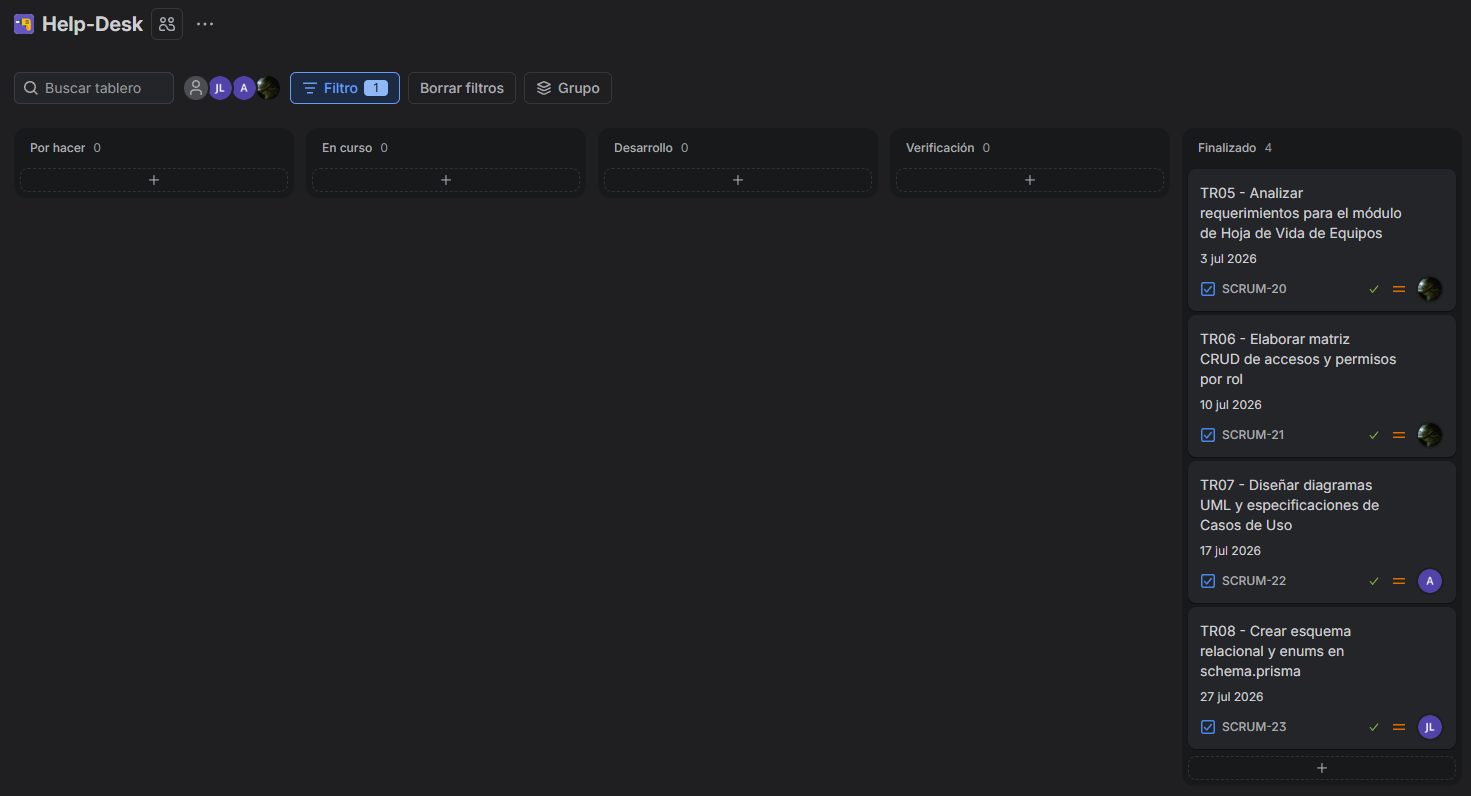
\includegraphics[width=0.92\textwidth]{tablero_sprint_1.png}
\\[0.2em]
{\small \textit{Nota.} Vista general del tablero de tareas correspondiente al análisis detallado, diagramas UML y configuración inicial Backend}
\end{figure}

\begin{figure}[H]
\centering
\captionsetup{justification=centering}
\caption{Burndown Chart - Sprint 1}
\label{fig:burndown_sprint_1}
\vspace{0.2em}
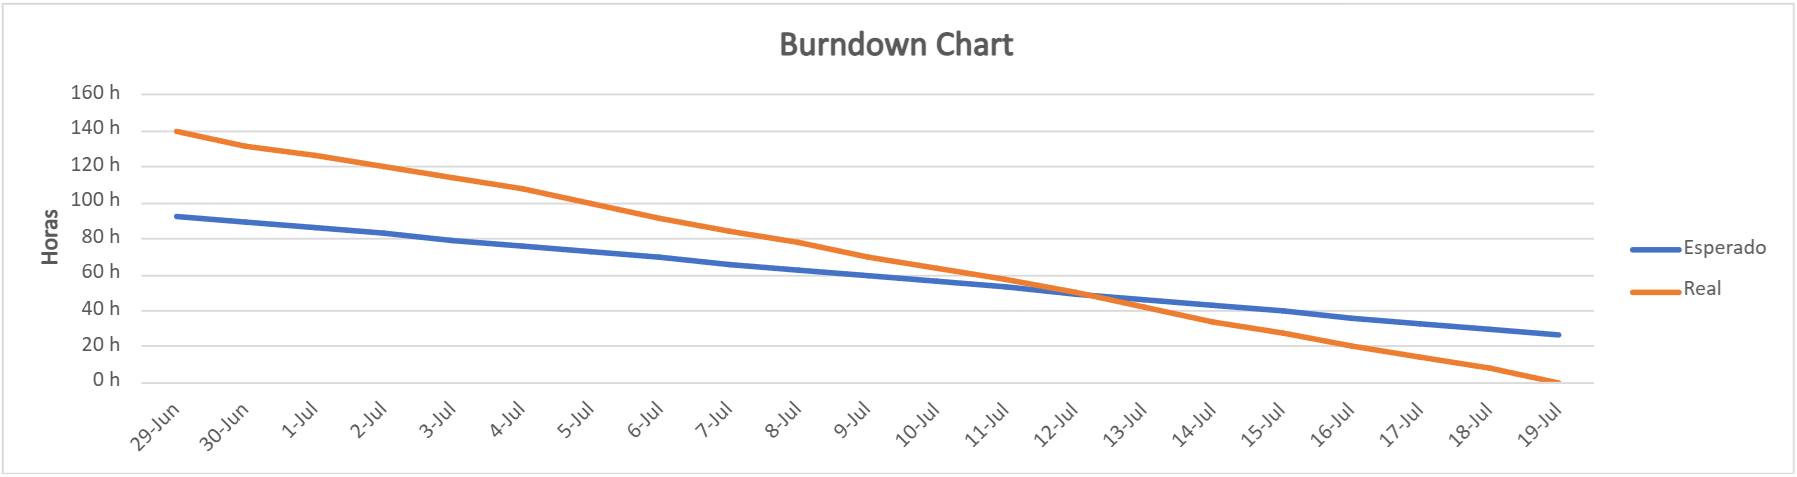
\includegraphics[width=0.92\textwidth]{burdowchart_sprint1.png}
\\[0.2em]
{\small \textit{Nota.} Elaboración propia. Seguimiento de horas estimadas frente al avance real durante el Sprint 1.}
\end{figure}

\begin{figure}[H]
\centering
\captionsetup{justification=centering}
\caption{Esquema Relacional implementado en \texttt{schema.prisma}}
\label{fig:evidencia_schema_prisma}
\vspace{0.2em}
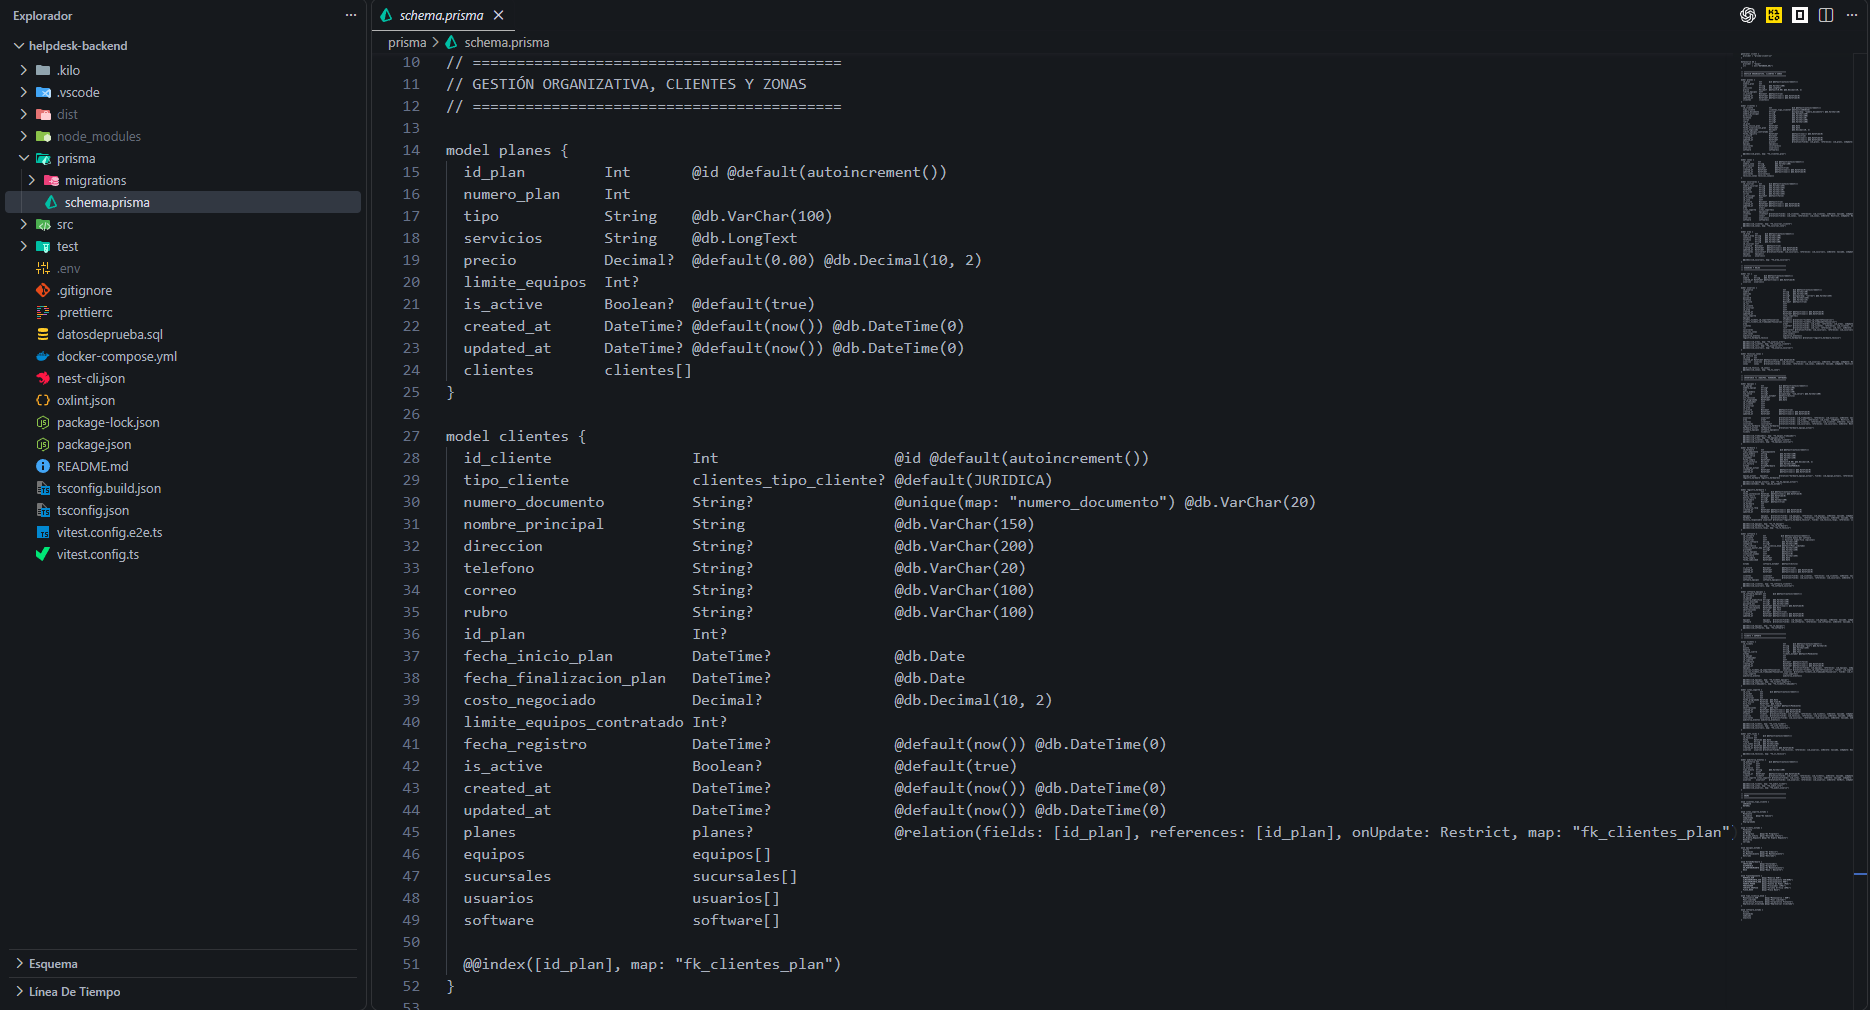
\includegraphics[width=0.92\textwidth]{schema_prisma.png}
\\[0.2em]
{\small \textit{Nota.} Definición de modelos, entidades y enumeraciones relacionales en el archivo de configuración de Prisma.}
\end{figure}

\subsubsection{Fase 2: Backend Core y Módulos Iniciales (Sprints 2 - 3)}
Durante esta etapa se ejecuta la construcción principal de la lógica del servidor, implementando los módulos de autenticación segura, gestión de usuarios, clientes, sucursales, planes SLA y el control transaccional del inventario ITAM, cuyas tareas ejecutadas se presentan en la Tabla \ref{tab:fase2}.

\begingroup
\small
\renewcommand{\arraystretch}{1.25}
\begin{longtable}{@{} p{3.2cm} p{8.8cm} p{3.0cm} @{}}
\caption{{Fase 2: Backend Core y Módulos Iniciales (Sprints 2 - 3)}} \label{tab:fase2} \\
\toprule
\textbf{Actividad / Tarea} & \textbf{Descripción del Entregable} & \textbf{Duración / Plazo} \\
\midrule
\endfirsthead

\multicolumn{3}{@{}l}{\textbf{Tabla \ref{tab:fase2}} \textit{(Continuación)}} \\[0.4em]
\toprule
\textbf{Actividad / Tarea} & \textbf{Descripción del Entregable} & \textbf{Duración / Plazo} \\
\midrule
\endhead

\midrule
\multicolumn{3}{r}{\textit{Continúa en la siguiente página\dots}} \\
\endfoot

\bottomrule
\multicolumn{3}{@{}p{\textwidth}}{\small \textit{Nota.} Cronograma y entregables detallados para el desarrollo del núcleo del backend.} \\
\endlastfoot

TR09 - Configuración NestJS & Configuración con Arquitectura Hexagonal, Prisma Client y módulo Common. & 5 días \\
TR10 - Autenticación JWT & Desarrollo de Autenticación JWT y Guards de Control de Acceso por Roles. & 5 días \\
TR11 - CRUD Usuarios y Zonas & Implementación de CRUD de Usuarios, Zonas geográficas y Auditoría. & 6 días \\
TR12 - Backend Clientes & Desarrollo del backend de Clientes con flujo de confirmación por correo. & 5 días \\
TR13 - Sucursales y Áreas & Gestión de Sucursales/Áreas y provisión de usuario por sucursal. & 5 días \\
TR14 - Gestión SLA & Implementación de gestión backend de Planes y Acuerdos de Nivel de Servicio. & 5 días \\
TR15 - Lógica Inventario ITAM & Desarrollo de lógica backend de Inventario ITAM y Hoja de Vida de Activos. & 6 días \\
TR16 - Control de Software & Implementación de gestión backend de Software y Control de Licencias. & 5 días \\
TR17 - Ciclo de Vida Ticket & Desarrollo del ciclo de vida del Ticket (estado pendiente y asignación). & 6 días \\
\textbf{Total Fase 2} & & \textbf{48 días} \\
\end{longtable}
\endgroup

Como evidencia de la ejecución del núcleo del servidor y gestión de inventario, se muestran los tableros, los gráficos de seguimiento y la implementación técnica:

\begin{figure}[H]
\centering
\captionsetup{justification=centering}
\caption{Tablero de Jira - Sprint 2}
\label{fig:evidencia_sprint_2}
\vspace{0.2em}
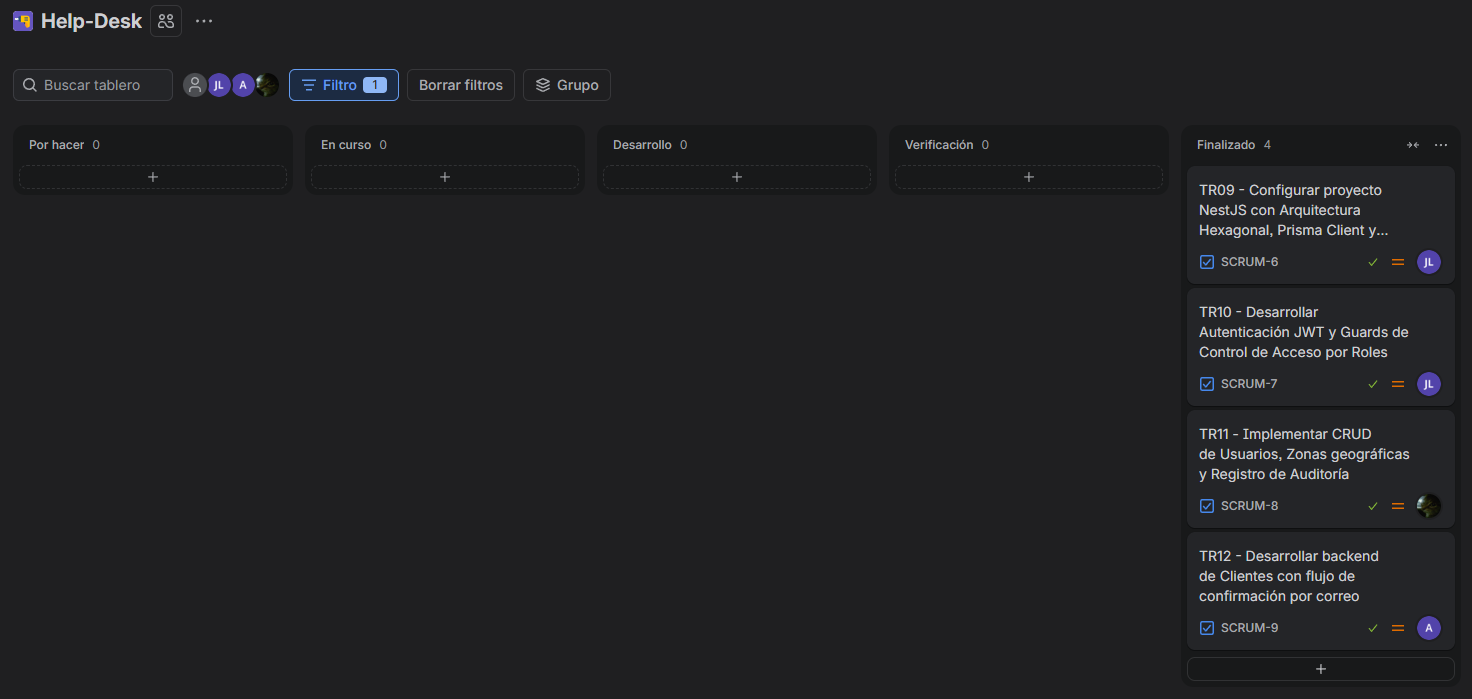
\includegraphics[width=0.92\textwidth]{tablero_sprint_2.png}
\\[0.2em]
{\small \textit{Nota.} Estado de avance del Backend en Autenticación, Usuarios y Jerarquía Organizacional.}
\end{figure}

\begin{figure}[H]
\centering
\captionsetup{justification=centering}
\caption{Burndown Chart - Sprint 2}
\label{fig:burndown_sprint_2}
\vspace{0.2em}
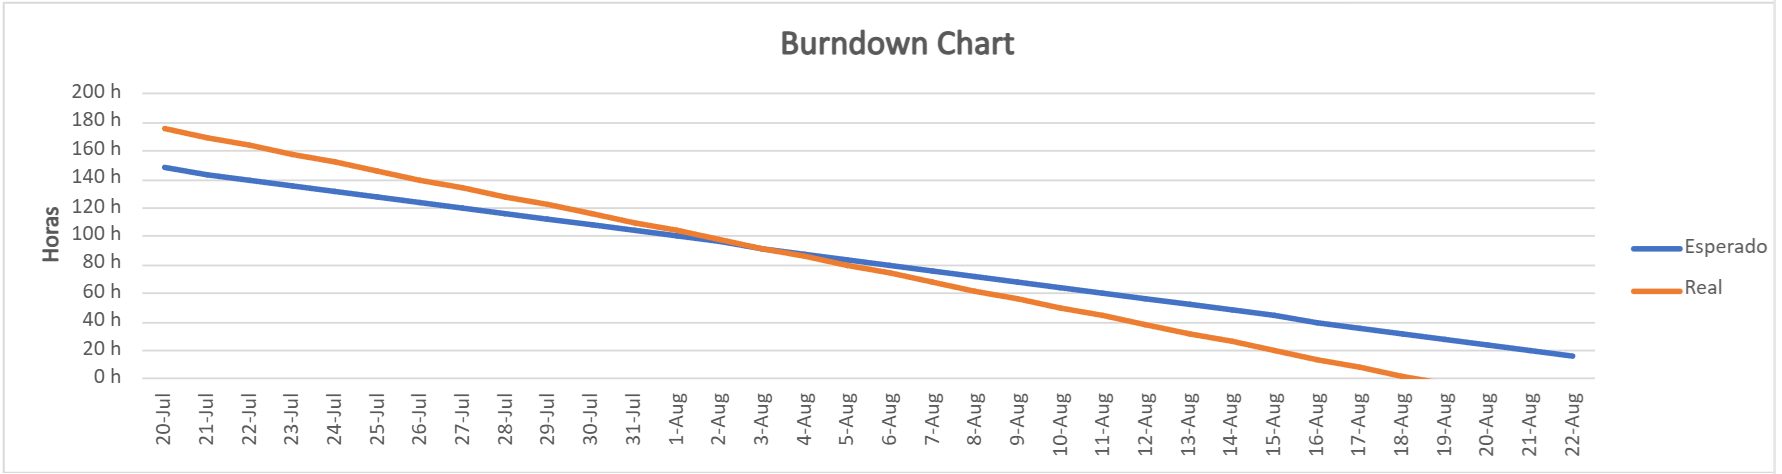
\includegraphics[width=0.92\textwidth]{burdowchart_sprint2.png}
\\[0.2em]
{\small \textit{Nota.} Elaboración propia. Seguimiento de horas estimadas frente al avance real durante el Sprint 2.}
\end{figure}

\begin{figure}[H]
\centering
\captionsetup{justification=centering}
\caption{Tablero de Jira - Sprint 3}
\label{fig:evidencia_sprint_3}
\vspace{0.2em}
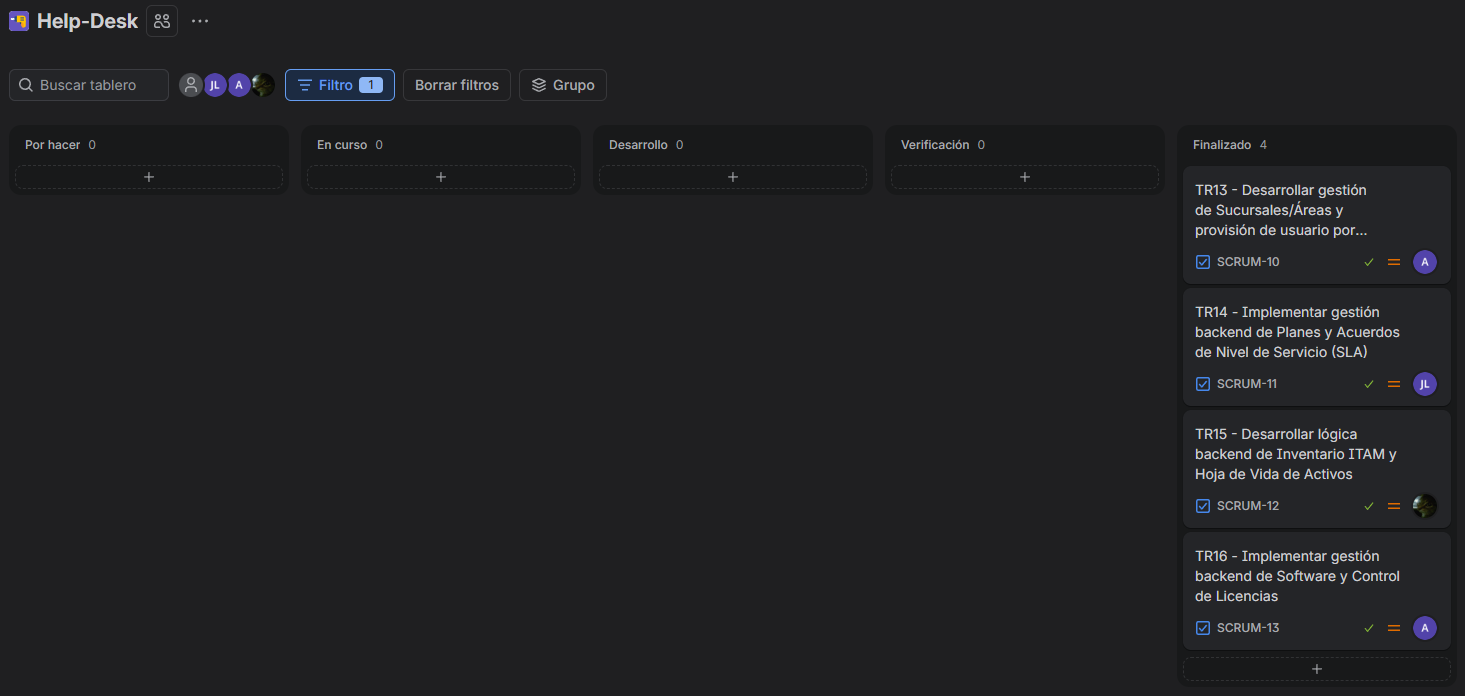
\includegraphics[width=0.92\textwidth]{img/tablero_sprint_3.png}
\\[0.2em]
{\small \textit{Nota.} Estado de avance del Backend en Sucursales, SLA, Inventario ITAM y Licencias.}
\end{figure}

\begin{figure}[H]
\centering
\captionsetup{justification=centering}
\caption{Burndown Chart - Sprint 3}
\label{fig:burndown_sprint_3}
\vspace{0.2em}
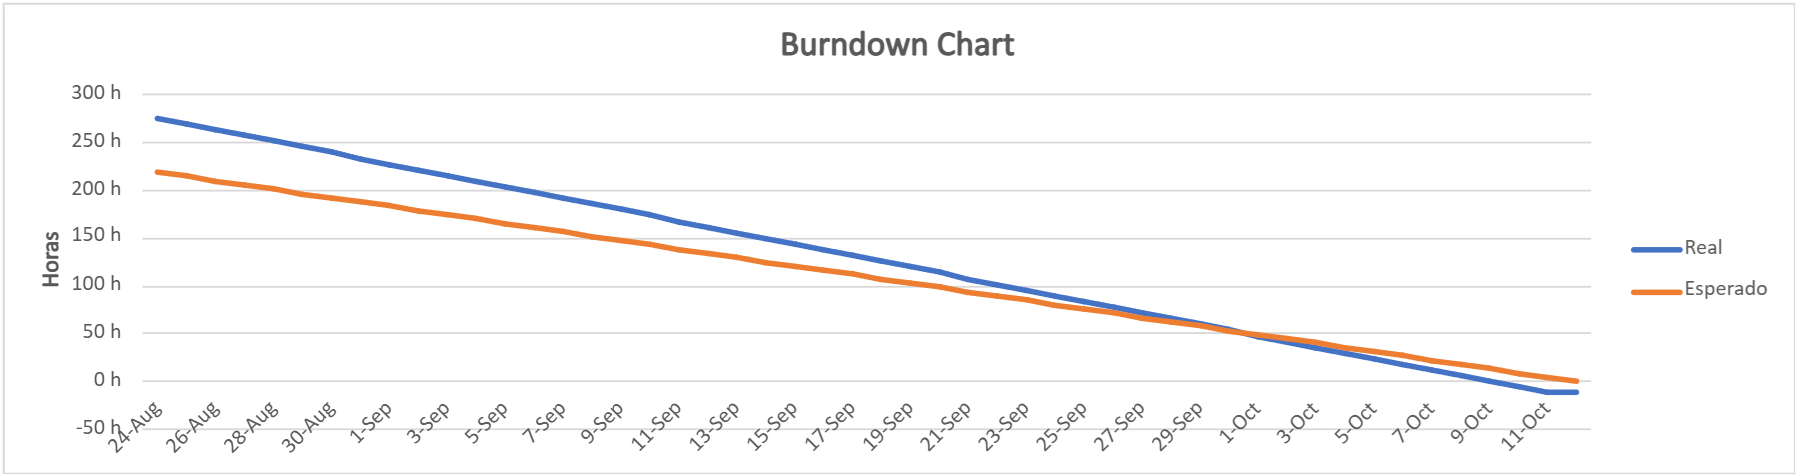
\includegraphics[width=0.92\textwidth]{burdowchart_sprint3.png}
\\[0.2em]
{\small \textit{Nota.} Elaboración propia. Seguimiento de horas estimadas frente al avance real durante el Sprint 3.}
\end{figure}

\begin{figure}[H]
\centering
\captionsetup{justification=centering}
\caption{Evidencia de ejecución de tareas del backend en NestJS}
\label{fig:evidencia_tarea_backend}
\vspace{0.2em}
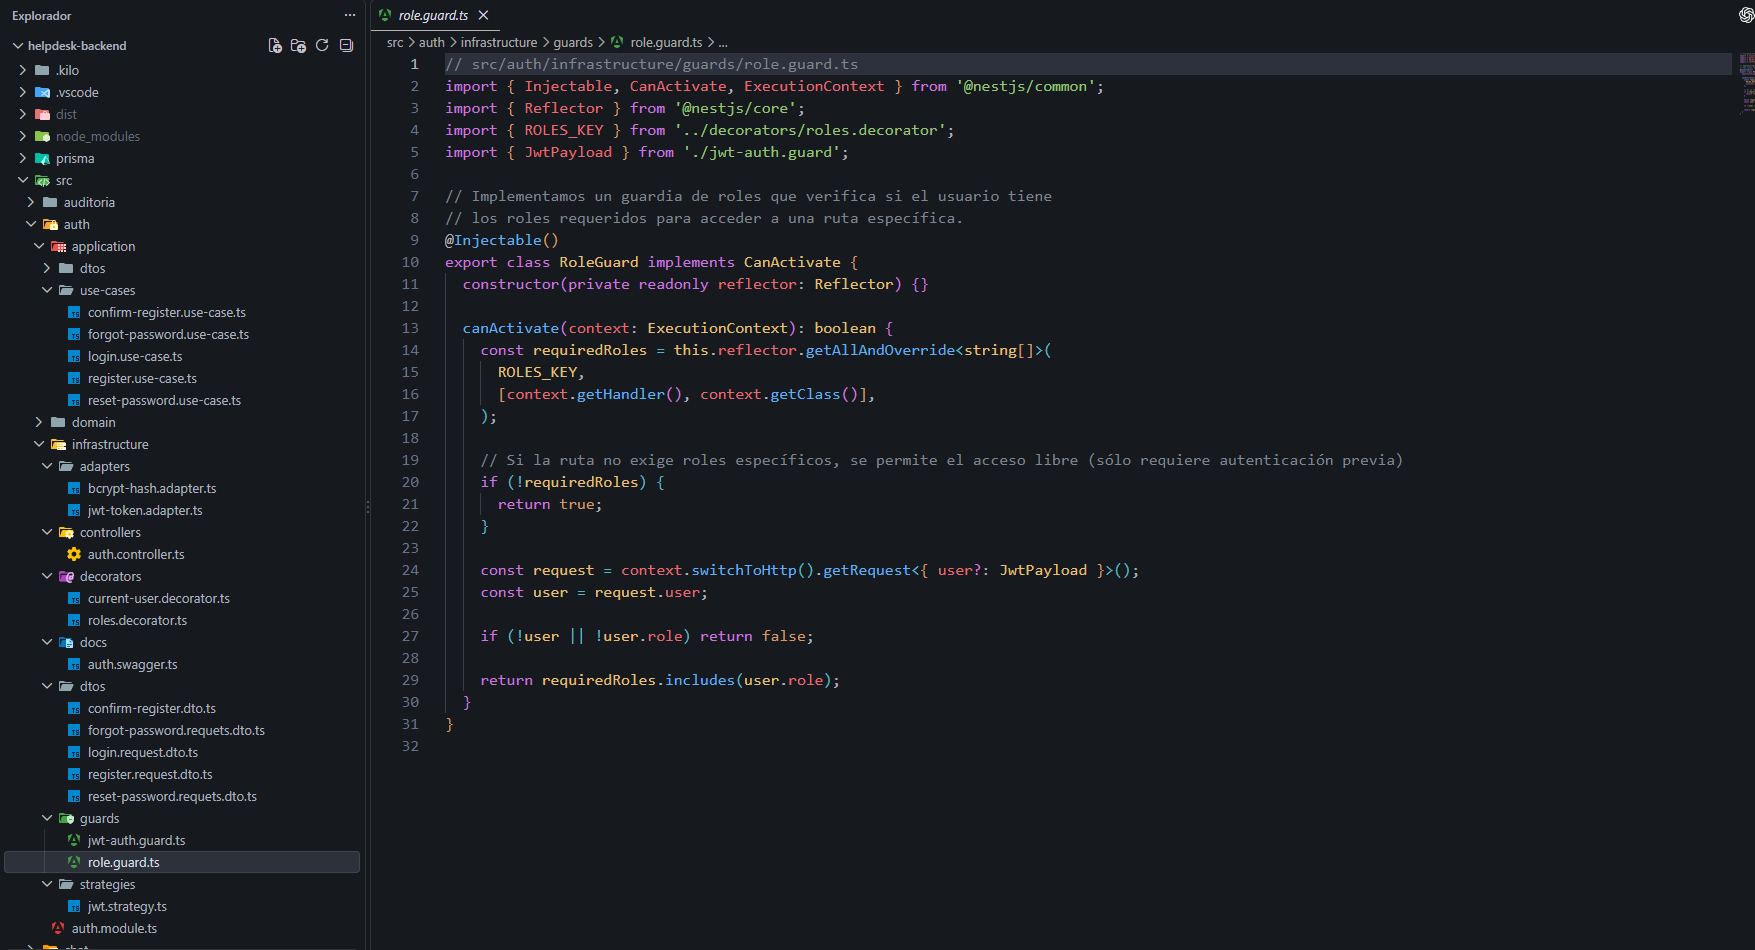
\includegraphics[width=0.92\textwidth]{evidencia_tarea_sprint_2_3.png}
\\[0.2em]
{\small \textit{Nota.} Implementación de controladores, servicios y Guards de seguridad basados en roles (RBAC).}
\end{figure}

\subsubsection{Fase 3: Backend Avanzado, Motor de Asignación y Tiempo Real (Sprint 4)}
Esta fase comprende el desarrollo de la lógica compleja de negocio, integrando el motor de derivación de citas presenciales, comunicación bidireccional mediante WebSockets y caché en Redis, cuyo resumen de actividades se observa en la Tabla \ref{tab:fase3}.

\begingroup
\small
\renewcommand{\arraystretch}{1.25}
\begin{longtable}{@{} p{3.2cm} p{8.8cm} p{3.0cm} @{}}
\caption{{Fase 3: Backend Avanzado, Motor de Asignación y Tiempo Real (Sprint 4)}} \label{tab:fase3} \\
\toprule
\textbf{Actividad / Tarea} & \textbf{Descripción del Entregable} & \textbf{Duración / Plazo} \\
\midrule
\endfirsthead

\multicolumn{3}{@{}l}{\textbf{Tabla \ref{tab:fase3}} \textit{(Continuación)}} \\[0.4em]
\toprule
\textbf{Actividad / Tarea} & \textbf{Descripción del Entregable} & \textbf{Duración / Plazo} \\
\midrule
\endhead

\midrule
\multicolumn{3}{r}{\textit{Continúa en la siguiente página\dots}} \\
\endfoot

\bottomrule
\multicolumn{3}{@{}p{\textwidth}}{\small \textit{Nota.} Actividades correspondientes al desarrollo del motor de citas y comunicación en tiempo real.} \\
\endlastfoot

TR18 - Citas Presenciales & Desarrollo del backend de derivación y gestión de Citas Presenciales. & 5 días \\
TR19 - WebSockets y Redis & Implementación de WebSockets con Redis para Chat y Endpoints de Dashboard. & 6 días \\
\textbf{Total Fase 3} & & \textbf{11 días} \\
\end{longtable}
\endgroup

Como evidencia de esta fase avanzada, se adjuntan el tablero de Jira, el gráfico de seguimiento y la lógica de programación del motor de citas:

\begin{figure}[H]
\centering
\captionsetup{justification=centering}
\caption{Tablero de Jira - Sprint 4 (Motor de Citas y WebSockets)}
\label{fig:evidencia_sprint_4}
\vspace{0.2em}
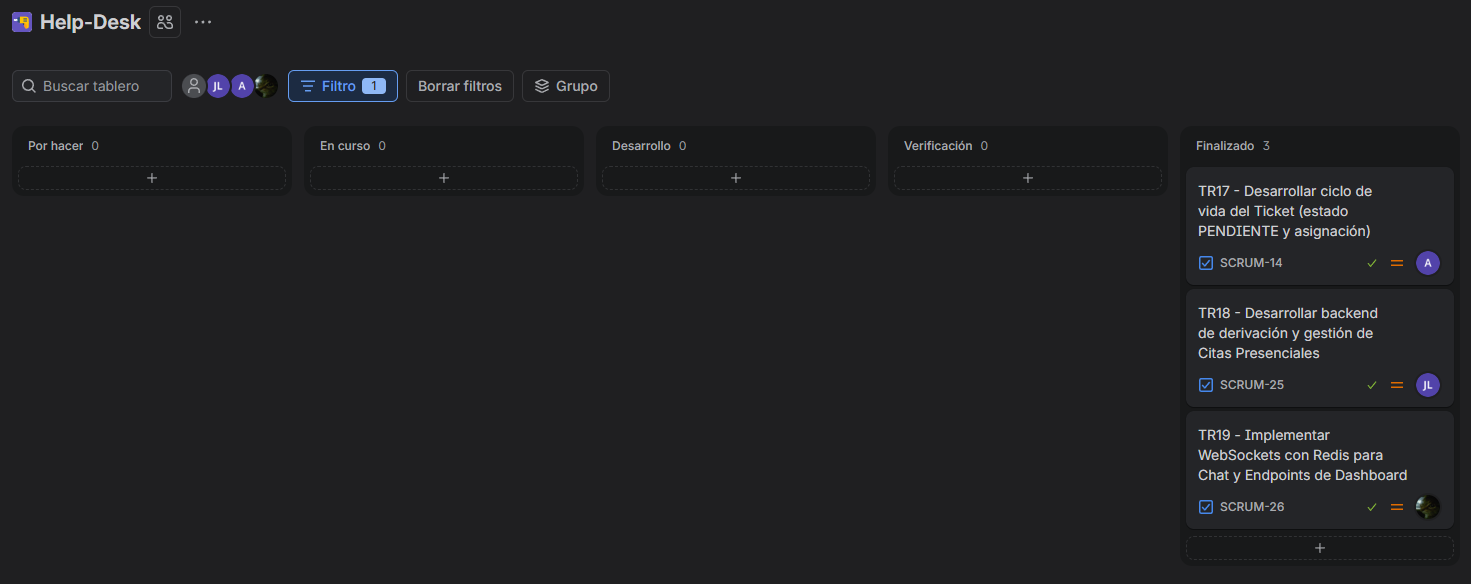
\includegraphics[width=0.92\textwidth]{tablero_sprint_4.png}
\\[0.2em]
{\small \textit{Nota.} Tablero de gestión de tareas para la lógica avanzada de negocio y comunicación en tiempo real.}
\end{figure}

\begin{figure}[H]
\centering
\captionsetup{justification=centering}
\caption{Burndown Chart - Sprint 4}
\label{fig:burndown_sprint_4}
\vspace{0.2em}
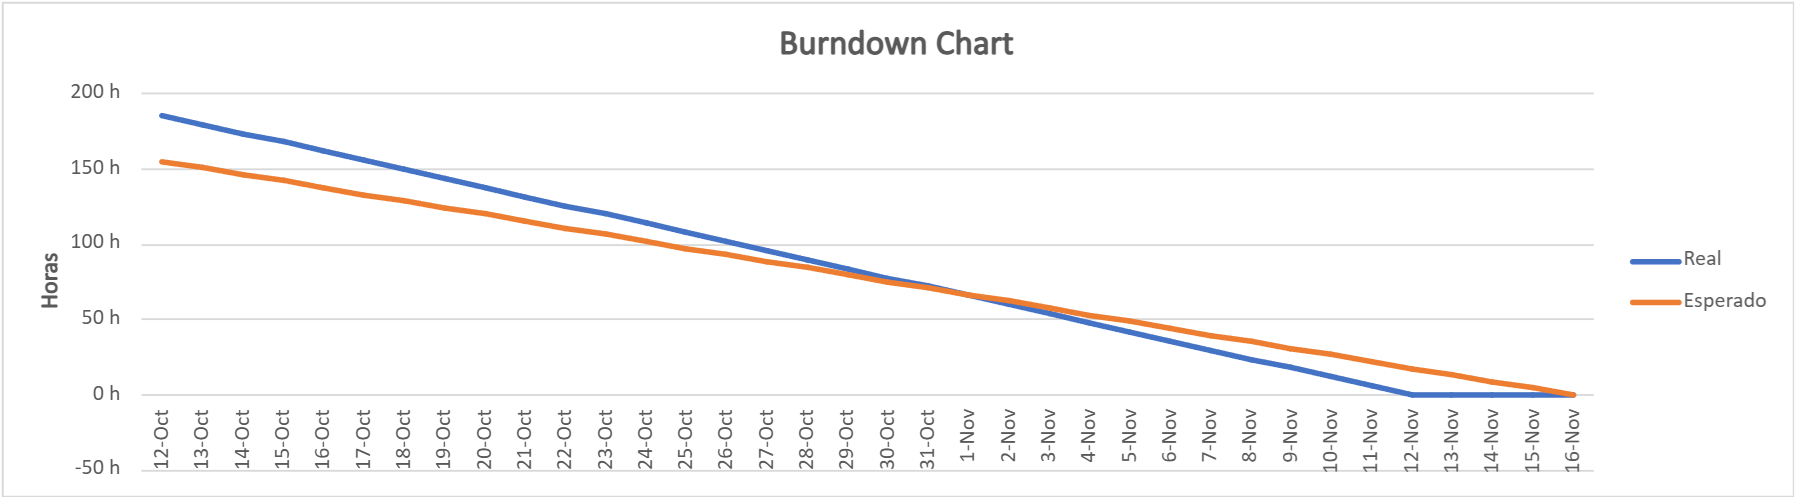
\includegraphics[width=0.92\textwidth]{burdowchart_sprint4.png}
\\[0.2em]
{\small \textit{Nota.} Elaboración propia. Seguimiento de horas estimadas frente al avance real durante el Sprint 4.}
\end{figure}

\begin{figure}[H]
\centering
\captionsetup{justification=centering}
\caption{Evidencia del motor de citas y control anti-cruces}
\label{fig:evidencia_tarea_sprint_4}
\vspace{0.2em}
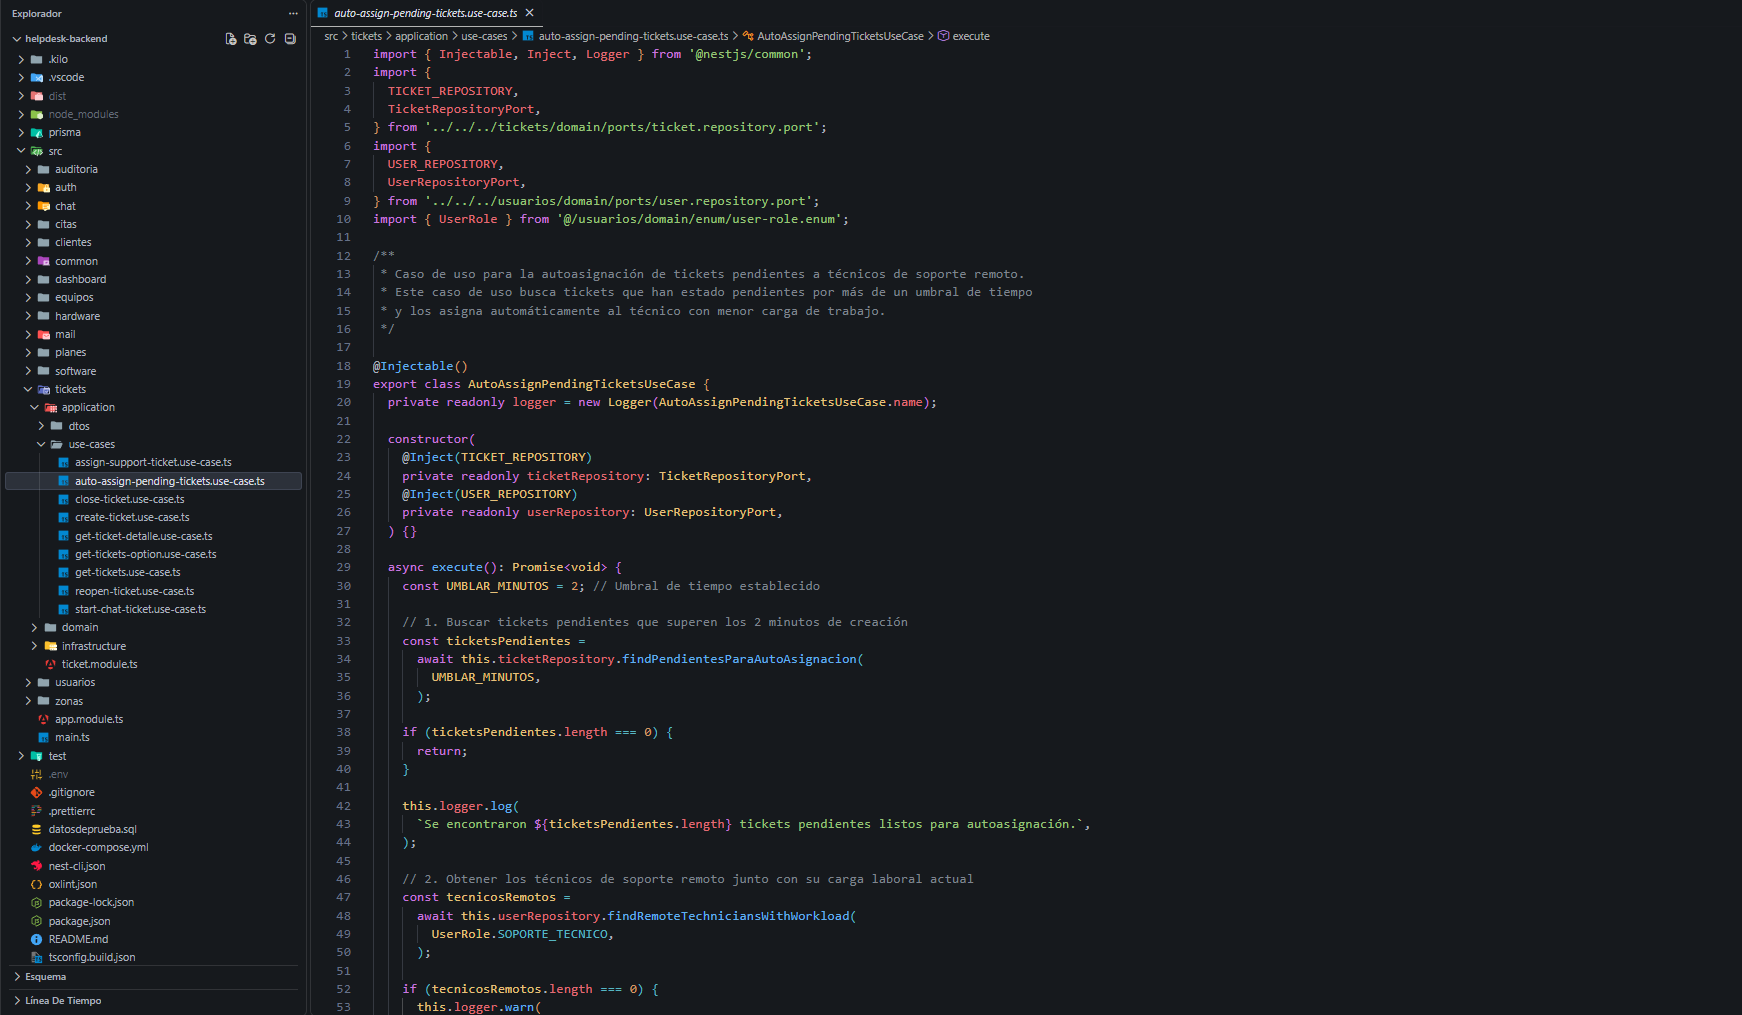
\includegraphics[width=0.92\textwidth]{evidencia_tarea_sprint_4.png}
\\[0.2em]
{\small \textit{Nota.} Implementación del algoritmo de autoasignación por zonas geográficas y gestión de franjas horarias.}
\end{figure}

\subsubsection{Fase 4: Frontend e Interfaces de Usuario (Sprint 5)}
Se enfoca en la implementación del diseño responsivo y la construcción de las pantallas de interacción mediante Next.js y componentes estilizados, estructurando paneles modulares por roles cuyas actividades se reflejan en la Tabla \ref{tab:fase4}.

\begingroup
\small
\renewcommand{\arraystretch}{1.25}
\begin{longtable}{@{} p{3.2cm} p{8.8cm} p{3.0cm} @{}}
\caption{{Fase 4: Frontend e Interfaces de Usuario (Sprint 5)}} \label{tab:fase4} \\
\toprule
\textbf{Actividad / Tarea} & \textbf{Descripción del Entregable} & \textbf{Duración / Plazo} \\
\midrule
\endfirsthead

\multicolumn{3}{@{}l}{\textbf{Tabla \ref{tab:fase4}} \textit{(Continuación)}} \\[0.4em]
\toprule
\textbf{Actividad / Tarea} & \textbf{Descripción del Entregable} & \textbf{Duración / Plazo} \\
\midrule
\endhead

\midrule
\multicolumn{3}{r}{\textit{Continúa en la siguiente página\dots}} \\
\endfoot

\bottomrule
\multicolumn{3}{@{}p{\textwidth}}{\small \textit{Nota.} Tareas de diseño y desarrollo frontend con Next.js y componentes UI.} \\
\endlastfoot

TR20 - Configuración UI & Configuración de estructura modular frontend, Tailwind y componentes UI. & 4 días \\
TR21 - Pantallas Base Frontend & Desarrollo de pantallas frontend de Login, Usuarios y Zonas con \textit{shadcn/ui}. & 6 días \\
TR22 - Jerarquía Organizacional & Desarrollo de interfaces modulares para la Jerarquía Organizacional. & 5 días \\
TR23 - Módulos Operativos & Pantallas de Inventario ITAM, Tickets, Cronograma de Citas, Chat y Dashboard. & 7 días \\
\textbf{Total Fase 4} & & \textbf{22 días} \\
\end{longtable}
\endgroup

Como evidencia del desarrollo frontend, se presentan el tablero, el gráfico de seguimiento y las pantallas principales de la interfaz de usuario:

\begin{figure}[H]
\centering
\captionsetup{justification=centering}
\caption{Tablero de Jira - Sprint 5 (Frontend e Interfaces UI)}
\label{fig:evidencia_sprint_5}
\vspace{0.2em}
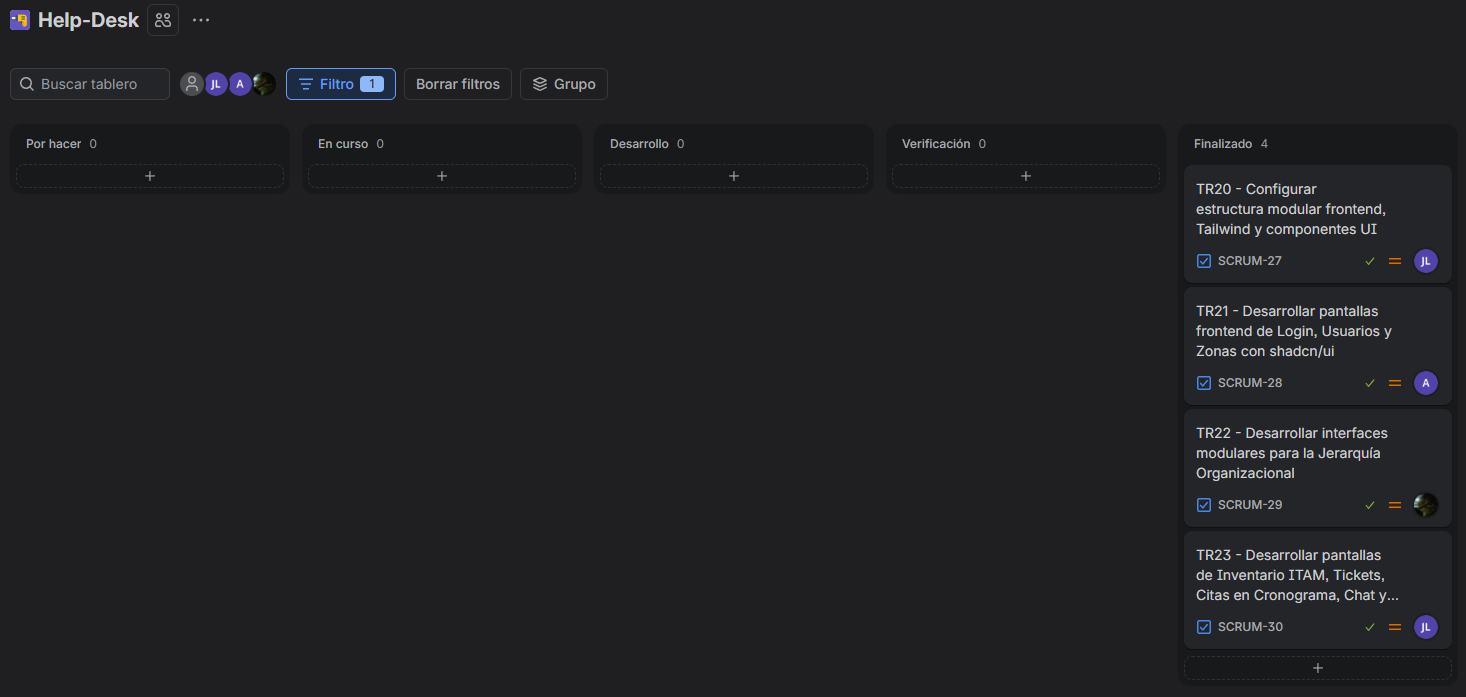
\includegraphics[width=0.92\textwidth]{tablero_sprint_5.png}
\\[0.2em]
{\small \textit{Nota.} Registro de tareas y componentes visuales desarrollados con Next.js y \textit{shadcn/ui}.}
\end{figure}

\begin{figure}[H]
\centering
\captionsetup{justification=centering}
\caption{Burndown Chart - Sprint 5}
\label{fig:burndown_sprint_5}
\vspace{0.2em}
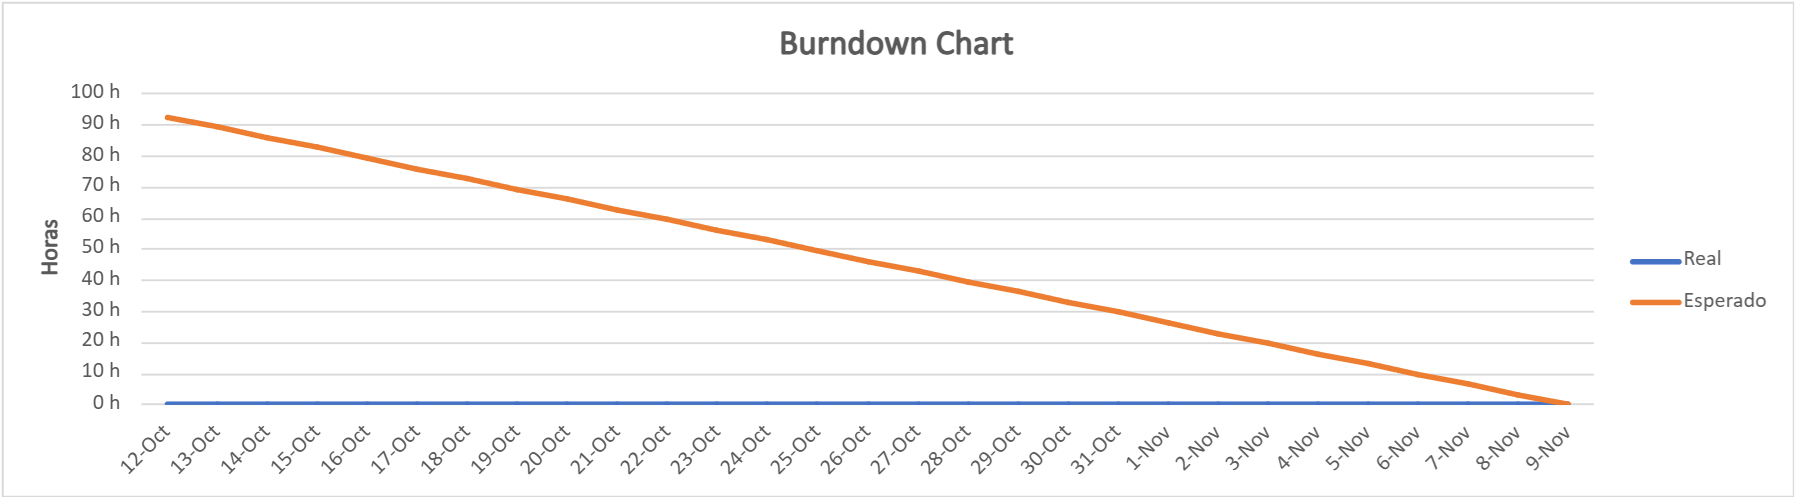
\includegraphics[width=0.92\textwidth]{burdowchart_sprint5.png}
\\[0.2em]
{\small \textit{Nota.} Elaboración propia. Seguimiento de horas estimadas frente al avance real durante el Sprint 5.}
\end{figure}

\begin{figure}[H]
\centering
\captionsetup{justification=centering}
\caption{Vistas operativas principales del sistema frontend (Dashboard - Administrador)}
\label{fig:evidencia_vistas_frontend_1}
\vspace{0.2em}
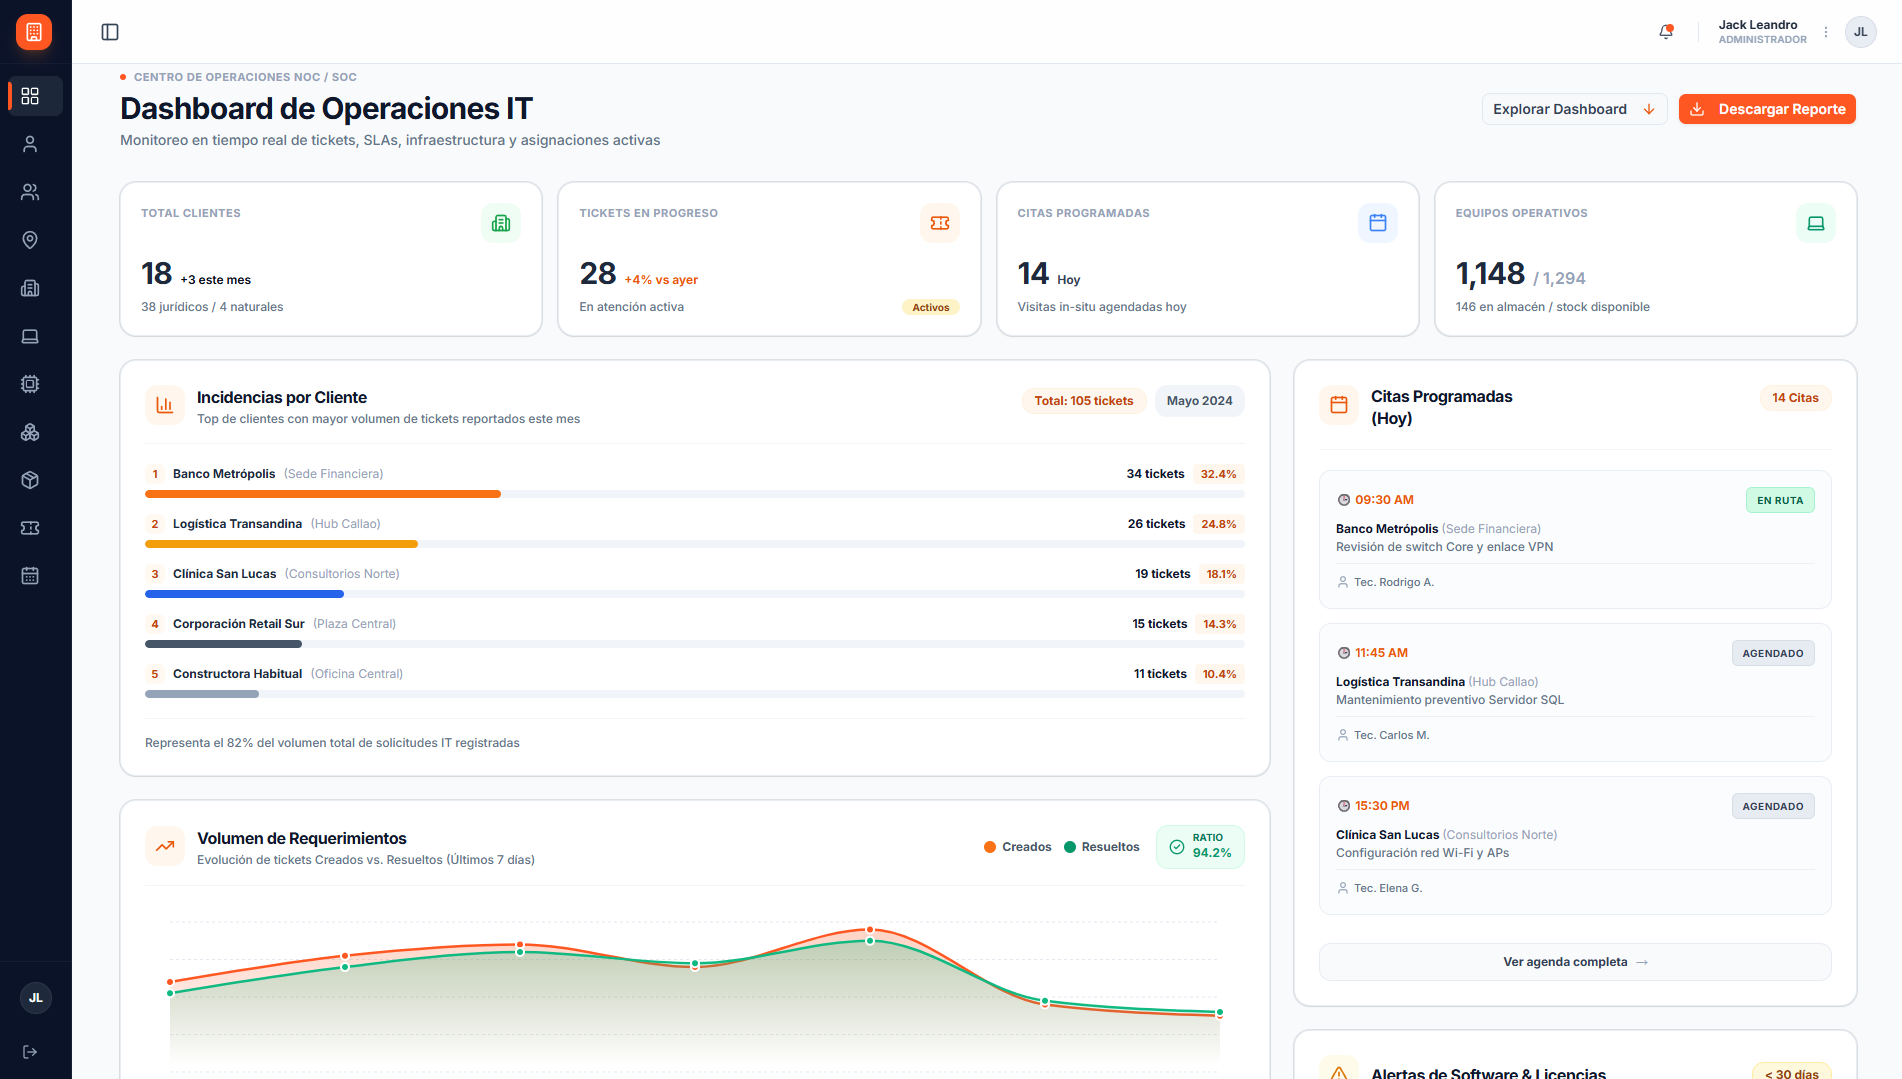
\includegraphics[width=0.92\textwidth]{img/evidencia_frontend_sprint_5_1.png}
\\[0.2em]
{\small \textit{Nota.} Pantallas clave correspondiente al panel de control.}
\end{figure}

\begin{figure}[H]
\centering
\captionsetup{justification=centering}
\caption{Vistas operativas principales del sistema frontend (Módulos Equipos ITAM)}
\label{fig:evidencia_vistas_frontend_2}
\vspace{0.2em}
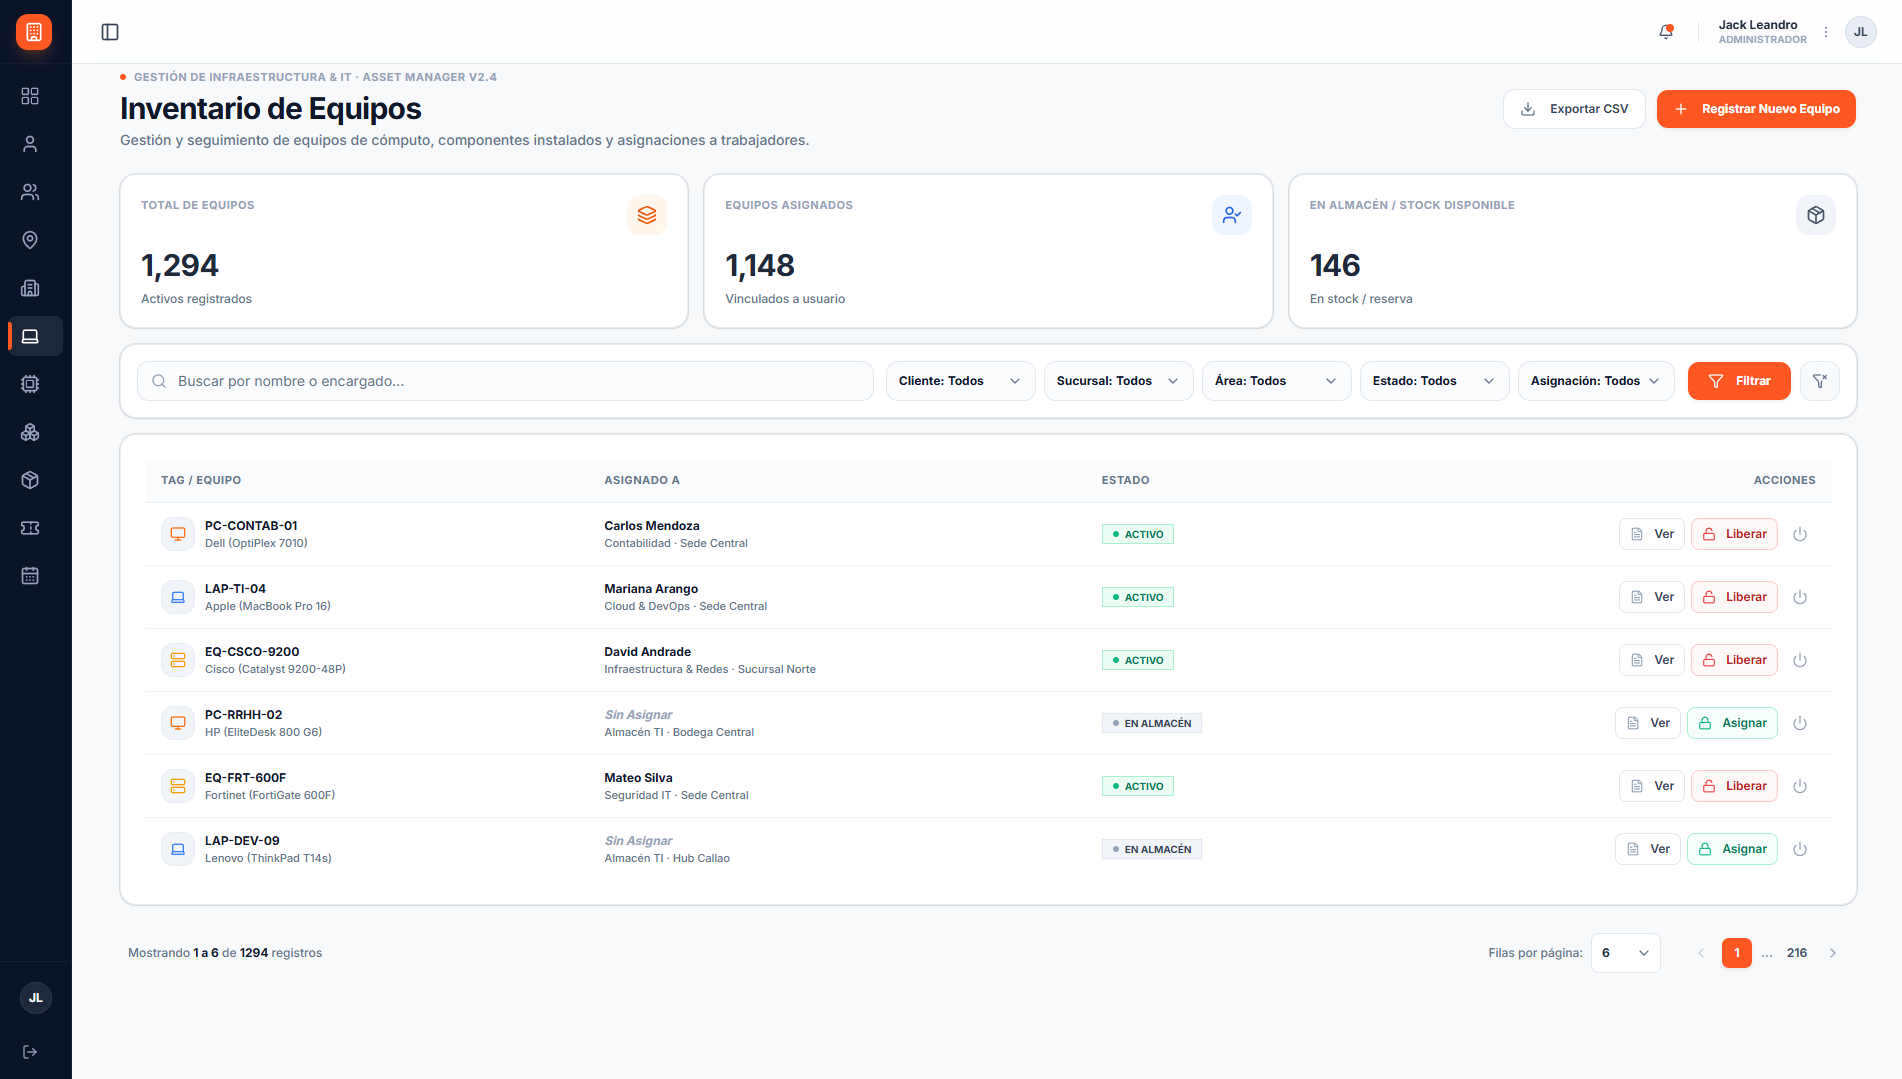
\includegraphics[width=0.92\textwidth]{img/evidencia_frontend_sprint_5_2.png}
\\[0.2em]
{\small \textit{Nota.} Pantallas clave correspondiente a gestión de equipos.}
\end{figure}

\begin{figure}[H]
\centering
\captionsetup{justification=centering}
\caption{Vistas operativas principales del sistema frontend (Módulos ITAM y Tickets)}
\label{fig:evidencia_vistas_frontend_3}
\vspace{0.2em}
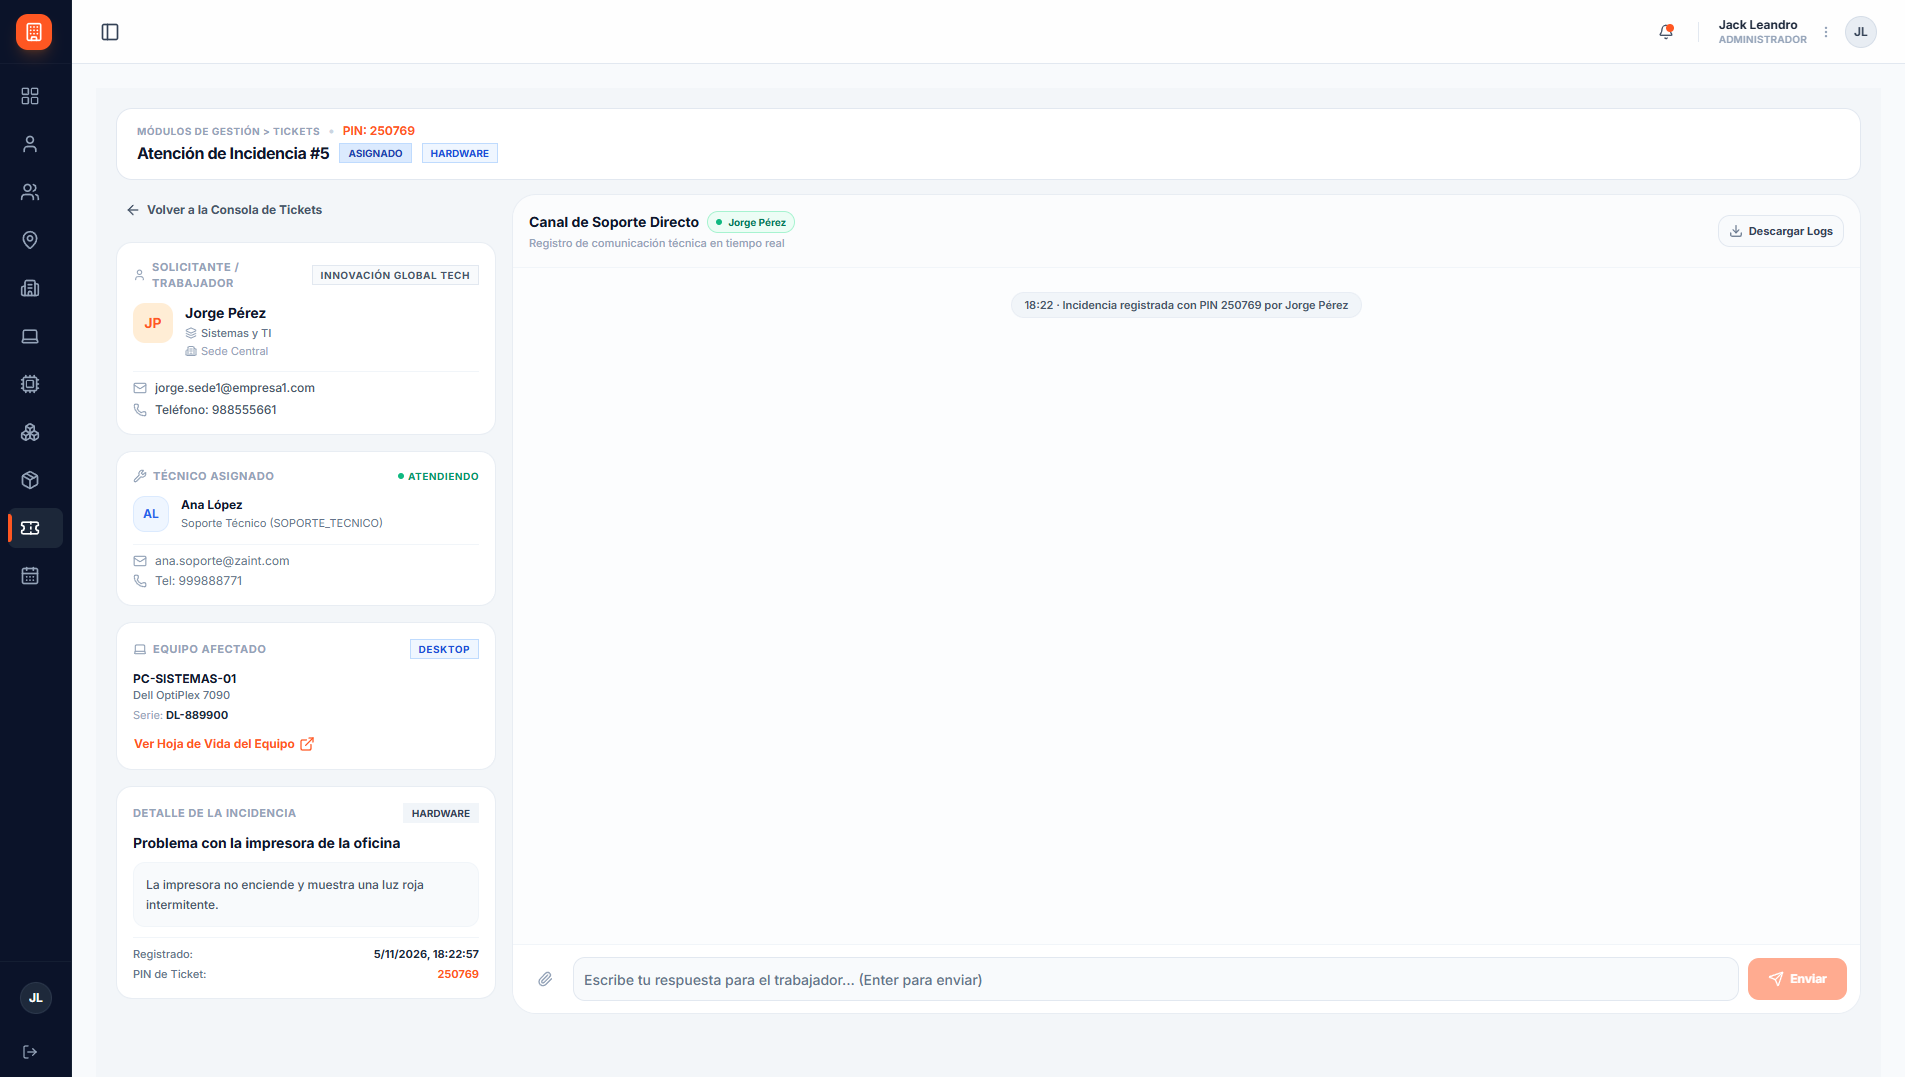
\includegraphics[width=0.92\textwidth]{img/evidencia_frontend_sprint_5_3.png}
\\[0.2em]
{\small \textit{Nota.} Pantallas clave correspondiente al ciclo de vida de ticket.}
\end{figure}

\subsubsection{Fase 5: Calidad, Documentación y Despliegue (Sprint 6)}
Fase final orientada a la validación mediante pruebas unitarias, documentación técnica de endpoints mediante Swagger y la puesta en producción del sistema, cuyas tareas se enumeran en la Tabla \ref{tab:fase5}.

\begingroup
\small
\renewcommand{\arraystretch}{1.25}
\begin{longtable}{@{} p{3.2cm} p{8.8cm} p{3.0cm} @{}}
\caption{{Fase 5: Calidad, Documentación y Despliegue (Sprint 6)}} \label{tab:fase5} \\
\toprule
\textbf{Actividad / Tarea} & \textbf{Descripción del Entregable} & \textbf{Duración / Plazo} \\
\midrule
\endfirsthead

\multicolumn{3}{@{}l}{\textbf{Tabla \ref{tab:fase5}} \textit{(Continuación)}} \\[0.4em]
\toprule
\textbf{Actividad / Tarea} & \textbf{Descripción del Entregable} & \textbf{Duración / Plazo} \\
\midrule
\endhead

\midrule
\multicolumn{3}{r}{\textit{Continúa en la siguiente página\dots}} \\
\endfoot

\bottomrule
\multicolumn{3}{@{}p{\textwidth}}{\small \textit{Nota.} Actividades de pruebas, documentación en Swagger y despliegue en producción.} \\
\endlastfoot

TR24 - Documentación Swagger & Documentación de endpoints y DTOs del Backend usando Swagger. & 4 días \\
TR25 - Pruebas Unitarias Jest & Implementación y ejecución de Pruebas Unitarias en el Backend con Jest. & 5 días \\
TR26 - Módulo de Exportación & Desarrollo de módulo de exportación de documentos PDF. & 5 días \\
TR27 - Despliegue en Producción & Subida de base de datos, backend y frontend al servidor de producción. & 4 días \\
\textbf{Total Fase 5} & & \textbf{18 días} \\
\end{longtable}
\endgroup

Para esta etapa final, se adjunta el tablero de seguimiento actual:

\begin{figure}[H]
\centering
\captionsetup{justification=centering}
\caption{Tablero de Jira - Sprint 6 (En Curso)}
\label{fig:evidencia_sprint_6}
\vspace{0.2em}
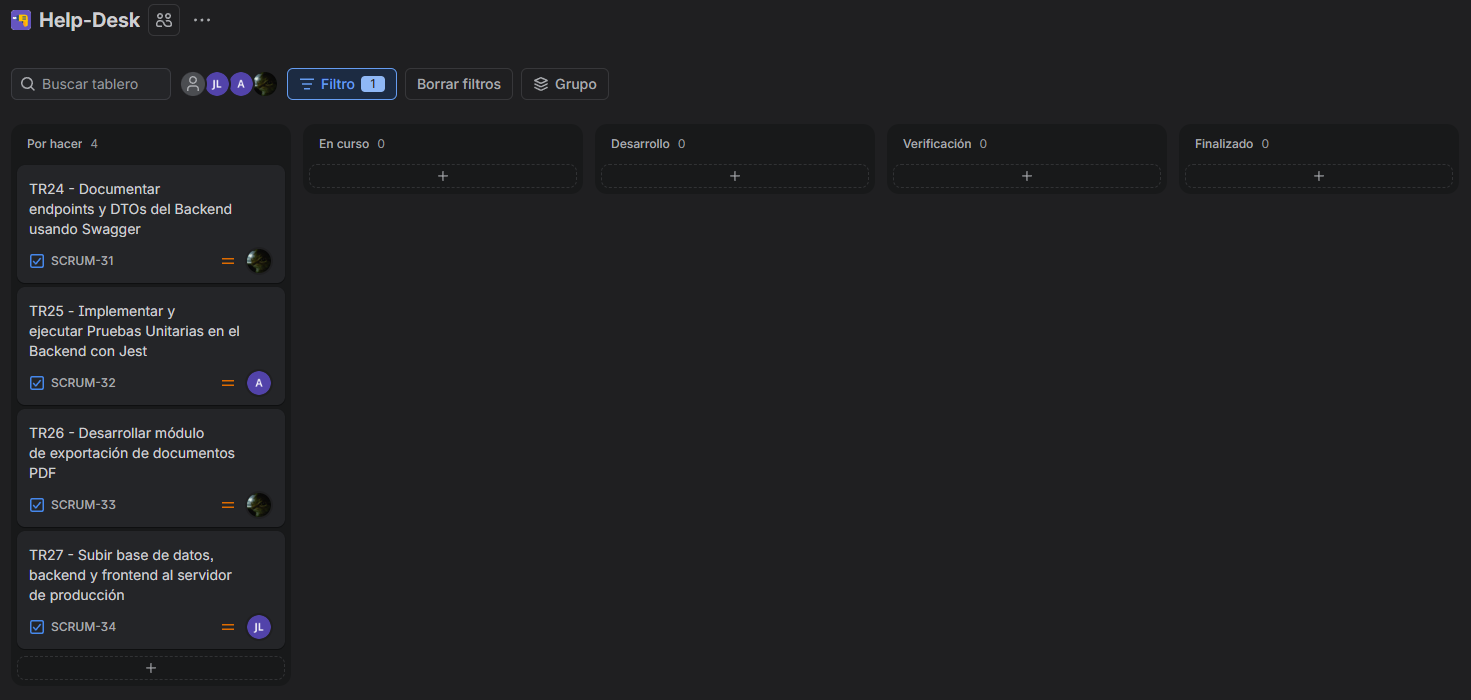
\includegraphics[width=0.92\textwidth]{tablero_sprint_6.png}
\\[0.2em]
{\small \textit{Nota.} Estado actual del tablero para las actividades de documentación en Swagger, pruebas unitarias y despliegue.}
\end{figure}

Nota: Las actividades correspondientes al Sprint 6 se encuentran actualmente en ejecución, abarcando las pruebas de integración finales y la puesta en producción del sistema web.

\section{Consideraciones técnicas, operativas y ambientales para la implementación de la mejora}

\subsection{Consideraciones Técnicas}
La arquitectura de la solución requiere compatibilidad con navegadores web modernos, protocolos de comunicación cifrada mediante HTTPS, autenticación basada en JSON Web Tokens (JWT) y una Arquitectura Modular Basada en Roles en el Frontend. El backend implementa NestJS, TypeScript, MySQL (con Prisma ORM) y Redis para la gestión transaccional y concurrente, aspecto fundamental para garantizar el correcto funcionamiento del algoritmo de reservas temporales (\textit{SoftLock}) y la autoasignación concurrente de citas.

\subsection{Consideraciones Operativas}
La puesta en marcha de la plataforma demanda una transición ordenada desde los canales informales (chats de WhatsApp, llamadas telefónicas) y registros dispersos en hojas de cálculo hacia el sistema Web Help-Desk centralizado. Esto optimiza de forma directa la operación diaria de la empresa J\&P Periféricos S.A.C. mediante los siguientes ejes operativos:

\begin{itemize}
\item \textbf{Formalización del Ingreso de Solicitudes:} Los usuarios finales ya no reportarán fallas por vías informales u opacas; cada incidencia generará formalmente un ticket de soporte asociado a un código PIN único, garantizando un registro centralizado y trazable.

\item \textbf{Inventario TI Centralizado y Hoja de Vida de Equipos:} El sistema integra la gestión detallada del parque informático corporativo organizado por empresas cliente, sucursales y áreas. Esto permite a los equipos de soporte consultar en tiempo real la \textbf{hoja de vida técnica} de cada equipo (historial de fallas, hardware instalado y licencias de software asignadas), brindando el contexto técnico necesario para agilizar la resolución de incidencias.

\item \textbf{Algoritmo Automatizado de Autoasignación y Derivación In-Situ:} 
El flujo operativo distingue claramente entre la atención remota y presencial:
\begin{itemize}
    \item Cuando el soporte remoto determina que la falla no puede resolverse de forma virtual, ejecuta la derivación hacia soporte presencial (\textit{in-situ}).
    \item El algoritmo de autoasignación analiza de forma automatizada los técnicos disponibles filtrando por la \textbf{zona geográfica de la sucursal}.
    \item Adicionalmente, el motor inteligente verifica si el técnico seleccionado ya cuenta con citas agendadas en la \textbf{misma sucursal}, priorizando y asignando esa misma franja horaria para agrupar hasta un máximo de tres (3) atenciones presenciales en una sola visita. Esto elimina desplazamientos innecesarios y optimiza los tiempos de traslado del personal técnico.
\end{itemize}

\item \textbf{Gestión de Componentes y Credenciales en Campo:} Durante las visitas presenciales, el técnico de soporte \textit{in-situ} gestiona dinámicamente la hoja de vida del equipo. Si se realiza el reemplazo o instalación de un nuevo componente de hardware (discos, memorias, etc.), el sistema registra la modificación de forma inmediata. Asimismo, el técnico cuenta con acceso controlado a las credenciales y claves de licencias de software requeridas para la intervención.

\item \textbf{Gestión del Cambio y Capacitación:} Se estructurará un plan de capacitación adaptado a cada perfil: inducción rápida para trabajadores finales (apertura de tickets), entrenamiento operativo para técnicos (gestión de hoja de vida y derivaciones), y uso de reportes y tableros métricos para la administración.

\end{itemize}

\subsection{Consideraciones Ambientales}
La implementación del sistema aporta beneficios directos desde la perspectiva ambiental y el desarrollo sostenible de las operaciones tecnológicas:
\begin{itemize}
\item \textbf{Reducción del Consumo de Papel y Suministros:} La digitalización integral del ciclo de vida de los tickets y los expedientes técnicos de hardware/software elimina drásticamente el uso de formularios físicos, cuadernos de registro manual e impresiones innecesarias de informes técnicos.
\item \textbf{Optimización de Desplazamientos y Menor Huella de Carbono:} Gracias al motor automatizado de asignación y agrupación de citas presenciales por zonas geográficas, se evitan viajes duplicados o traslados ineficientes del personal técnico. Esto disminuye el consumo de combustible de las unidades de transporte y reduce las emisiones de gases de efecto invernadero asociadas a la logística de campo.
\item \textbf{Eficiencia Energética en Infraestructura Digital:} Al centralizar los servicios sobre una arquitectura web optimizada (con gestión eficiente de consultas mediante caché en Redis), se reduce la sobrecarga de procesamiento local en equipos, promoviendo un menor consumo de energía eléctrica y prolongando la vida útil del parque informático de la empresa.
\end{itemize}

\section{Recursos técnicos para la implementación de la mejora}

Para garantizar el correcto desarrollo, despliegue y funcionamiento del sistema Web Help-Desk centralizado, se han estructurado los recursos técnicos en tres categorías esenciales:

\subsection{Infraestructura de Servidores y Conectividad}
\begin{itemize}
\item \textbf{Servidor de Alojamiento (Hosting):} Entorno de producción virtualizado en la nube con alta disponibilidad para hospedar los servicios del backend y frontend.
\item \textbf{Dominio y Protocolo SSL:} Dominio web propio con certificado de seguridad HTTPS para garantizar conexiones cifradas y proteger la integridad de los datos institucionales.
\item \textbf{Gestor de Mensajería en Tiempo Real:} Servidor Redis configurado para el manejo de canales de caché y soporte de eventos mediante WebSockets en las notificaciones y chats de soporte.
\end{itemize}

\subsection{Entorno de Desarrollo Software y Herramientas Tecnológicas}
\begin{itemize}
\item \textbf{Entorno Backend y Lenguaje:} Node.js como motor de ejecución y TypeScript como lenguaje tipado para el desarrollo de la API.
\item \textbf{Framework de Arquitectura:} NestJS estructurado bajo un enfoque modular y principios de código limpio.
\item \textbf{Entorno Frontend:} Next.js con Arquitectura Modular Basada en Roles para interfaces responsivas y dinámicas.
\item \textbf{Gestión de Bases de Datos:} MySQL para datos transaccionales mediante Prisma ORM, y MongoDB para el almacenamiento no relacional del historial de auditoría e interacciones.
\item \textbf{Control de Versiones y Documentación:} Git para la trazabilidad del código fuente y Swagger UI para la documentación interactiva de los endpoints.
\end{itemize}

\subsection{Hardware de Soporte y Estaciones de Trabajo}
\begin{itemize}
\item \textbf{Equipos de Computación:} Computadoras portátiles con procesadores de alto rendimiento, memoria RAM ampliada y discos de estado sólido (SSD) destinados a la codificación, compilación y pruebas locales del software.
\end{itemize}

\section{Diagrama del proceso, mapa del flujo de valor y/o diagrama de operación de la situación mejorada}
\subsection{Proceso de la empresa con la intervención del software}
Con la implementación de la solución tecnológica y el motor automatizado, el flujo de operaciones del área experimenta una automatización integral, reduciendo los tiempos de respuesta y centralizando las solicitudes de manera segura.

A continuación, se presentan los diagramas de procesos detallados por carriles (\textit{swimlanes}), redactados bajo notación de verbos en infinitivo y estructurados según el control de acceso basado en roles (RBAC) y la arquitectura multinivel del sistema:

\subsection{Proceso de Consulta de Hoja de Vida de Equipos (ITAM)}

El proceso de consulta de la hoja de vida de un activo informático permite la trazabilidad completa del historial de mantenimientos, componentes instalados y licencias asociadas. El acceso está determinado por el alcance del rol del usuario autenticado (Trabajador, Sucursal, Empresa o Soporte), garantizando que cada perfil consulte únicamente la información que le corresponde.

\begin{figure}[H]
\centering
\captionsetup{justification=centering}
\caption{Proceso de Consulta de Hoja de Vida de Equipos (ITAM)}
\label{fig:proceso_consulta_itam}
\vspace{0.2em}
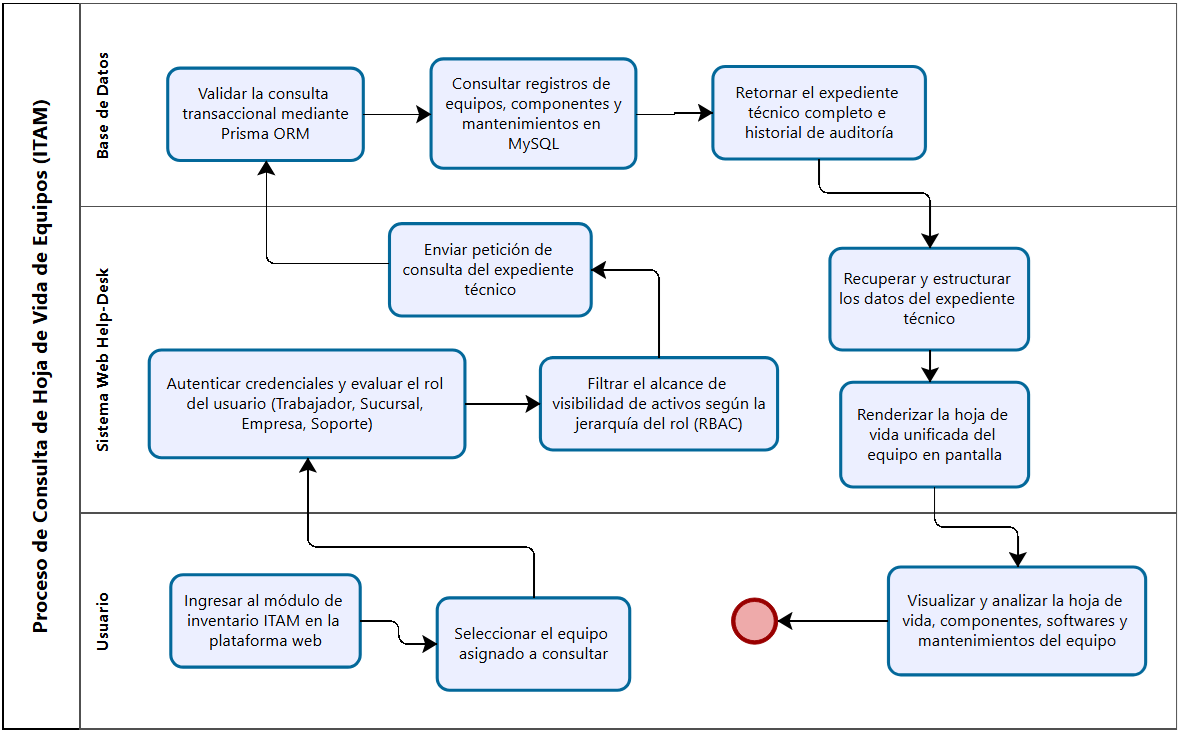
\includegraphics[width=0.92\textwidth]{Proceso de Consulta de Hoja de Vida de Equipos (ITAM).png}
\\[0.2em]
{\small \textit{Nota.} Esquema del flujo de consulta con filtrado de visibilidad por alcance de rol (RBAC) y respuesta transaccional mediante Prisma ORM.}
\end{figure}

\subsection{Proceso de Gestión y Registro de Hardware (ITAM)}

La administración física de los dispositivos tecnológicos contempla dos mecanismos principales de ingreso: el alta unitaria de componentes o equipos y la importación masiva por lotes mediante plantillas estandarizadas de Excel.

\begin{figure}[H]
\centering
\captionsetup{justification=centering}
\caption{Proceso de Gestión y Registro de Hardware (ITAM)}
\label{fig:proceso_gestion_hardware}
\vspace{0.4em}

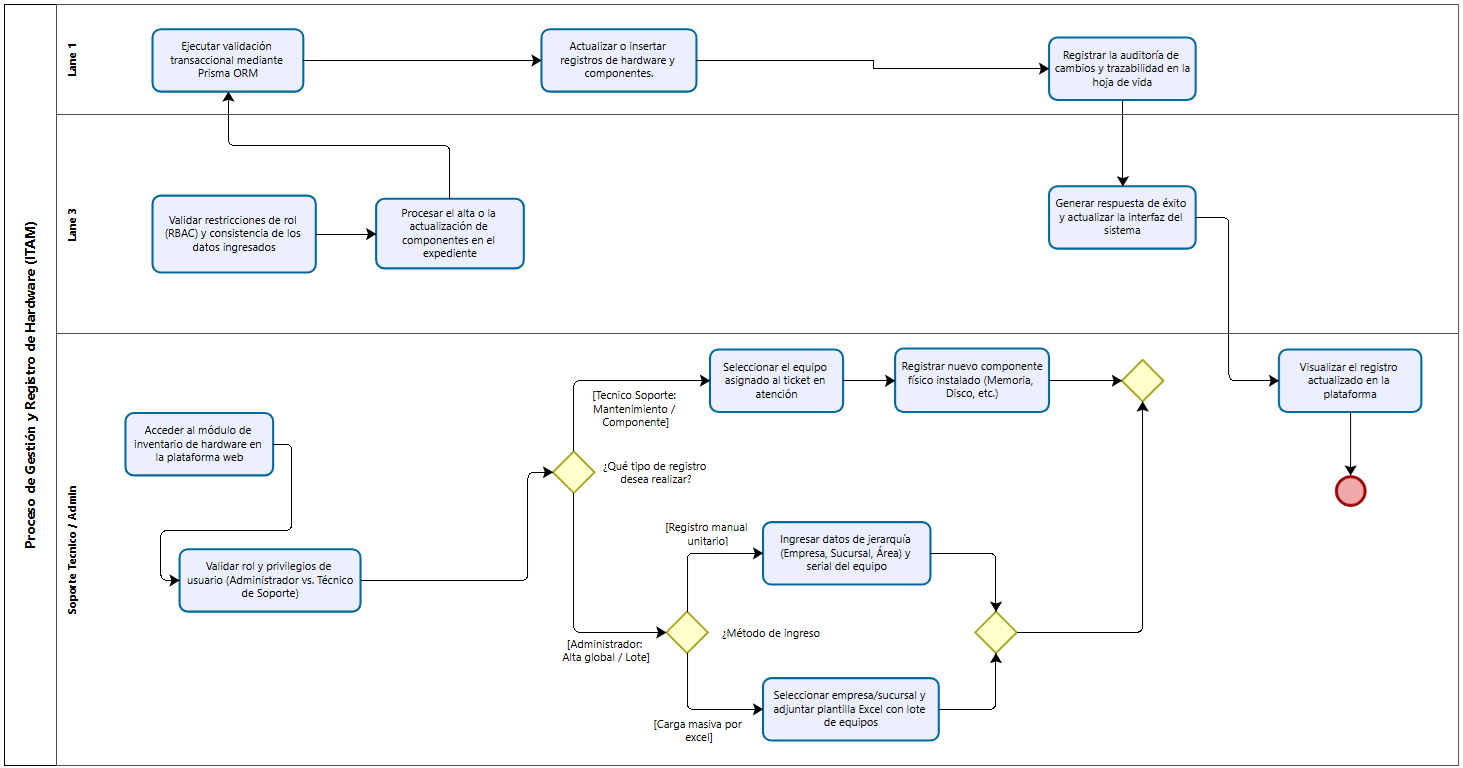
\includegraphics[width=0.95\textwidth]{Proceso de Gestión y Registro de Hardware (ITAM).png}

\vspace{0.4em}
{\small \textit{Nota.} Flujo de decisión entre registro unitario, carga por lote en Excel y mantenimiento por el técnico de soporte.}

\end{figure}

\subsection{Proceso de Gestión de Software y Licencias (ITAM)}

La gestión del catálogo de aplicaciones corporativas y asignación de licencias requiere un control riguroso del stock disponible para evitar sobrecostos o usos no autorizados.

\begin{figure}[H]
\centering
\captionsetup{justification=centering}
\caption{Proceso de Gestión de Software y Licencias (ITAM)}
\label{fig:proceso_gestion_software}
\vspace{0.4em}

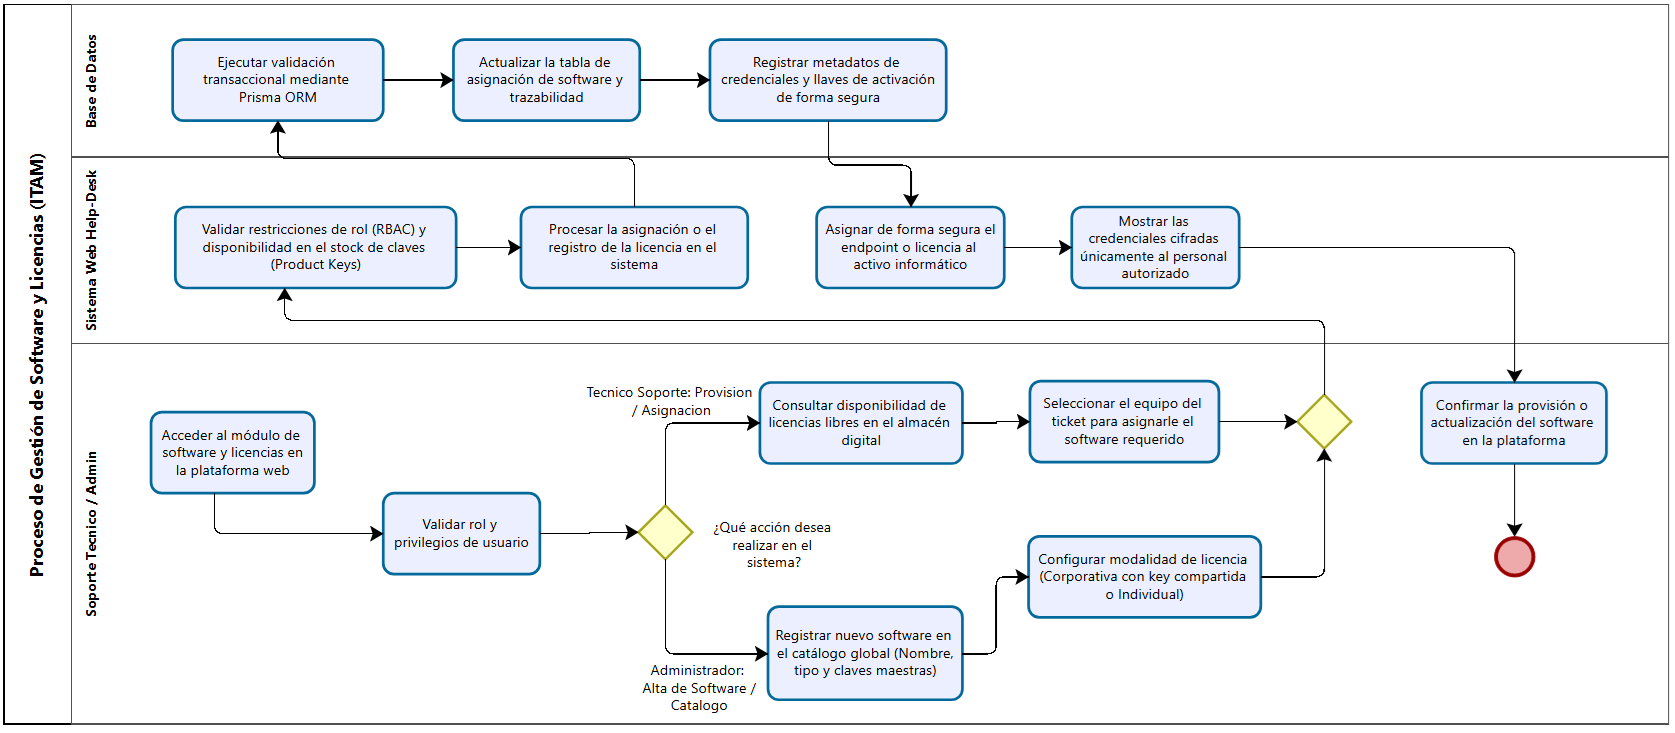
\includegraphics[width=0.95\textwidth]{Proceso de Gestión de Software y Licencias (ITAM).png}

\vspace{0.4em}
{\small \textit{Nota.} Representación del alta en el catálogo global y la asignación de claves de activación al activo correspondiente.}

\end{figure}

\subsection{Proceso de Gestión de Tickets y Soporte Técnico Remoto}

El flujo principal de atención remota ante incidencias tecnológicas inicia con la solicitud formal emitida por el trabajador, asignando de forma automatizada a un técnico disponible y ofreciendo comunicación directa.

\begin{figure}[H]
\centering
\captionsetup{justification=centering}
\caption{Proceso de Gestión de Tickets y Soporte Técnico Remoto}
\label{fig:proceso_tickets_soporte_remoto}
\vspace{0.4em}

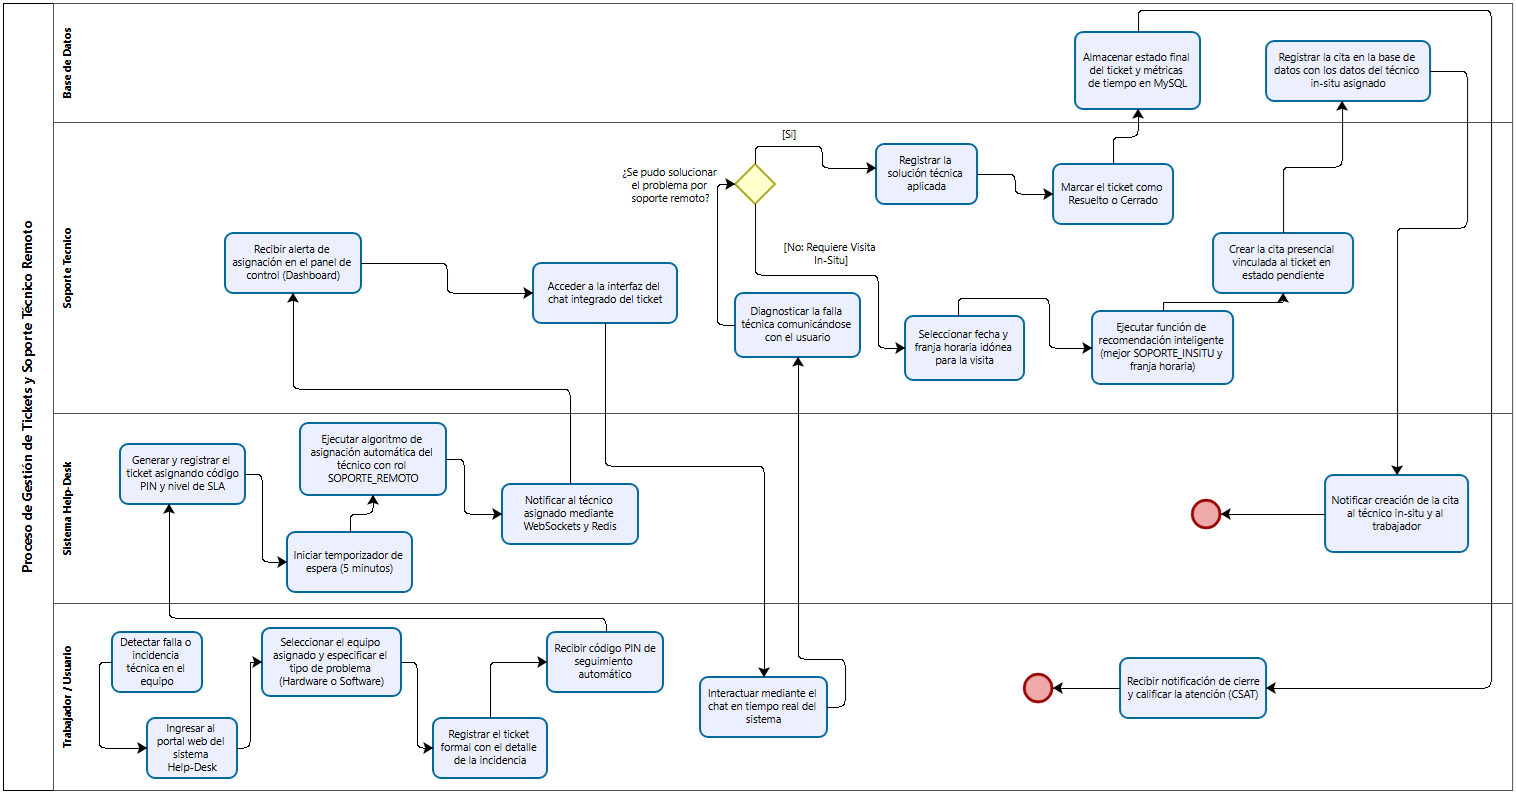
\includegraphics[width=0.95\textwidth]{Proceso de Gestión de Tickets y Soporte Técnico Remoto.png}

\vspace{0.4em}
{\small \textit{Nota.} Flujo transaccional desde el registro del ticket, la atención vía WebSockets y la derivación inteligente a soporte in-situ.}

\end{figure}

\subsection{Proceso de Soporte In-Situ y Ciclo de Vida de la Cita}

Para aquellas incidencias que demandan intervención física en las instalaciones de la empresa cliente, el sistema gestiona la asignación y el ciclo de estados de la visita presencial.

\begin{figure}[H]
\centering
\captionsetup{justification=centering}
\caption{Proceso de Soporte In-Situ y Ciclo de Vida de la Cita}
\label{fig:proceso_soporte_insitu}
\vspace{0.4em}

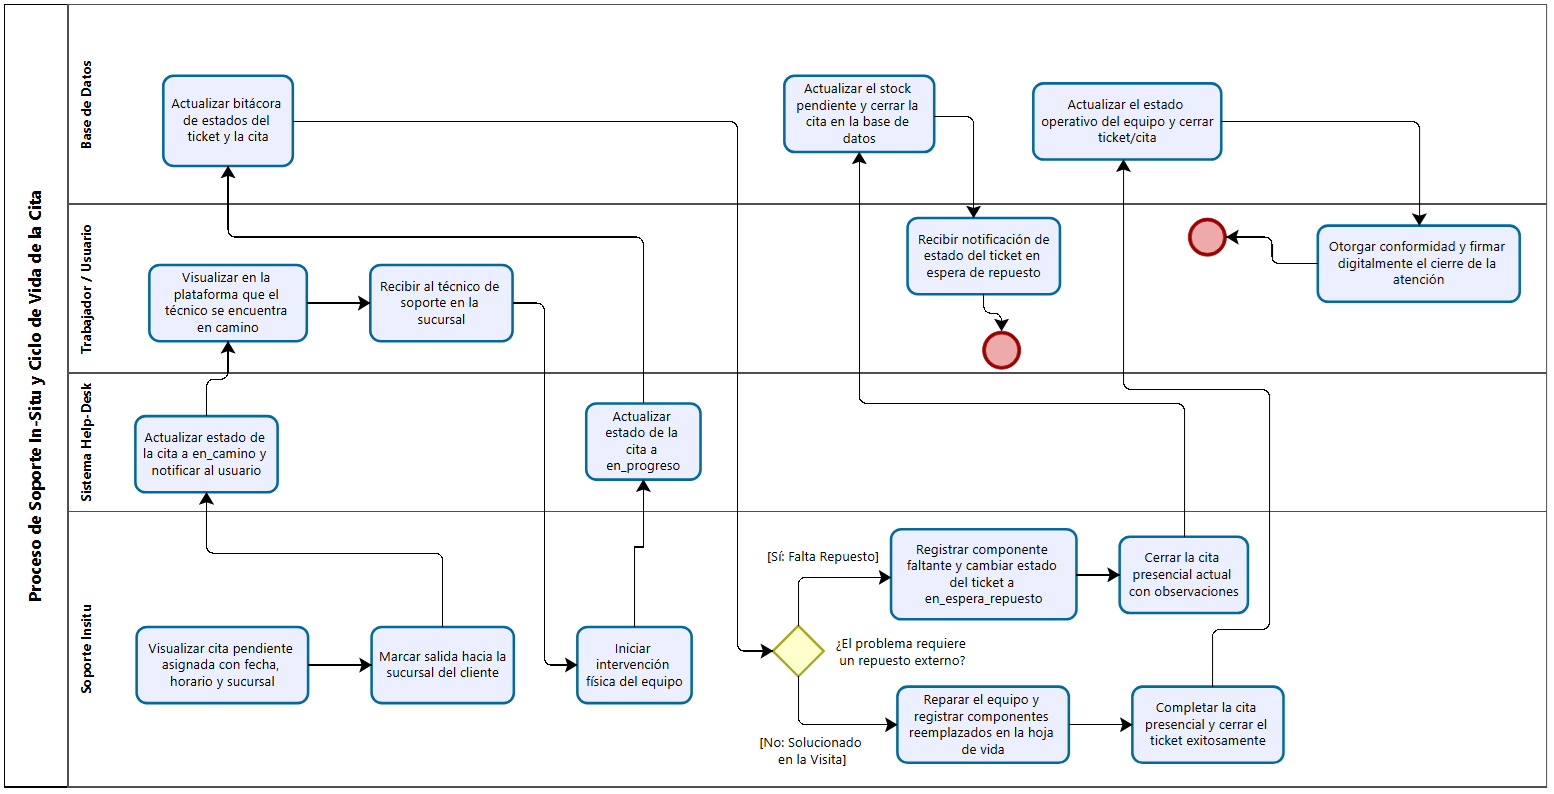
\includegraphics[width=0.95\textwidth]{Proceso de Soporte In-Situ y Ciclo de Vida de la Cita.png}

\vspace{0.4em}
{\small \textit{Nota.} Ciclo de vida de la cita presencial y atención según los escenarios de solución inmediata o espera de repuestos.}

\end{figure}

\section{Cronograma de ejecución de la mejora}
La ejecución del proyecto se proyecta en un período estructurado conforme al avance de los sprints de desarrollo:
\begin{enumerate}
\item \textbf{Sprint 1:} Análisis de requerimientos y diseño de arquitectura base (Prisma, entidades y roles).
\item \textbf{Sprint 2:} Desarrollo del backend, conexiones a base de datos, lógica de negocio, motor de autoasignación por zona y carga, y seguridad JWT.
\item \textbf{Sprint 3:} Desarrollo del frontend (Next.js), interfaces de usuario y paneles de control con arquitectura modular por roles, tableros Kanban y gestión de citas con \textit{SoftLock}.
\item \textbf{Sprint 4:} Pruebas de integración, validación de flujos de derivación, corrección de errores y despliegue final en producción.
\end{enumerate}

\newpage

A continuación, se presenta el diagrama de Gantt que detalla la planificación y el estado actual de las tareas del proyecto:

\begin{figure}[H]
\centering
\captionsetup{justification=centering}
\caption{Cronograma de Ejecución y Planificación del Proyecto (Parte 1)}
\label{fig:cronograma_ejecucion_1}
\vspace{0.3em}

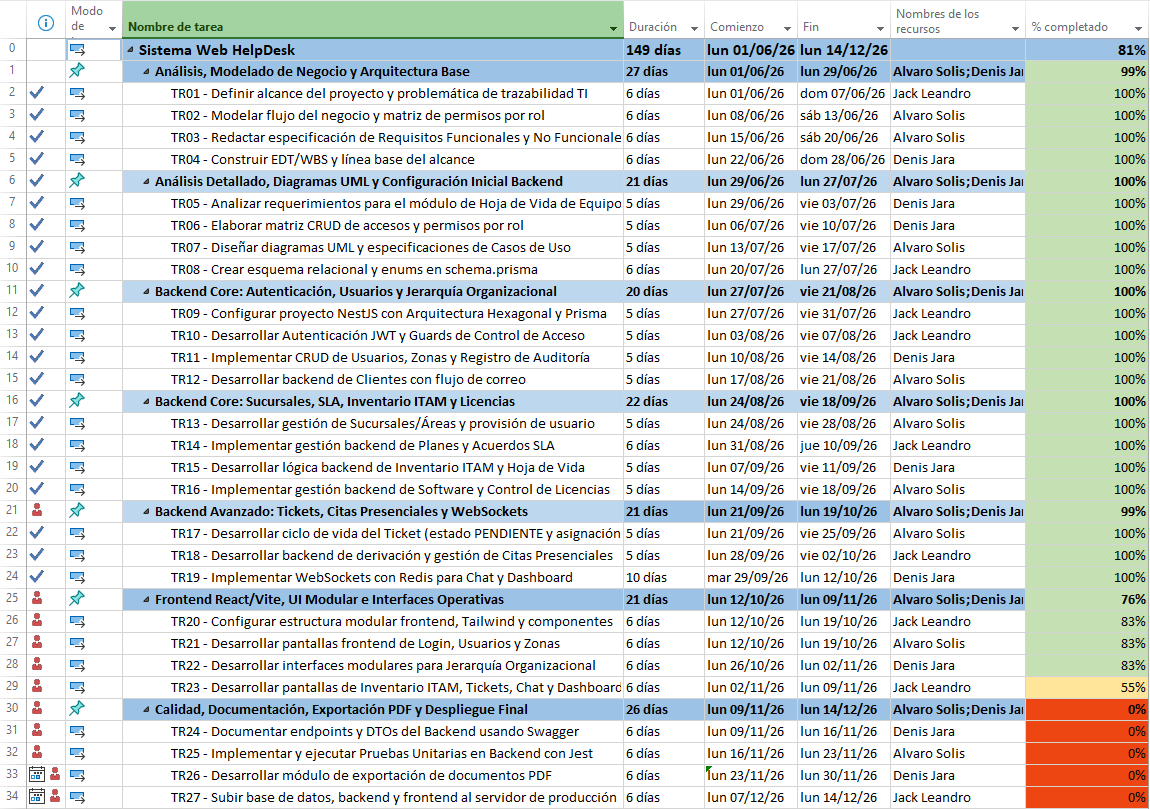
\includegraphics[width=0.98\textwidth, trim=0 0 0 0, clip]{Cronograma-Proyecto-1.png}

\vspace{-0.4em}
{\small \textit{Nota.} Elaboración propia basada en la planificación del sistema Help-Desk centralizado en Microsoft Project. Primera parte del cronograma.}

\end{figure}

\begin{figure}[H]
\centering
\captionsetup{justification=centering}
\caption{Cronograma de Ejecución y Planificación del Proyecto (Parte 2)}
\label{fig:cronograma_ejecucion_2}
\vspace{0.3em}

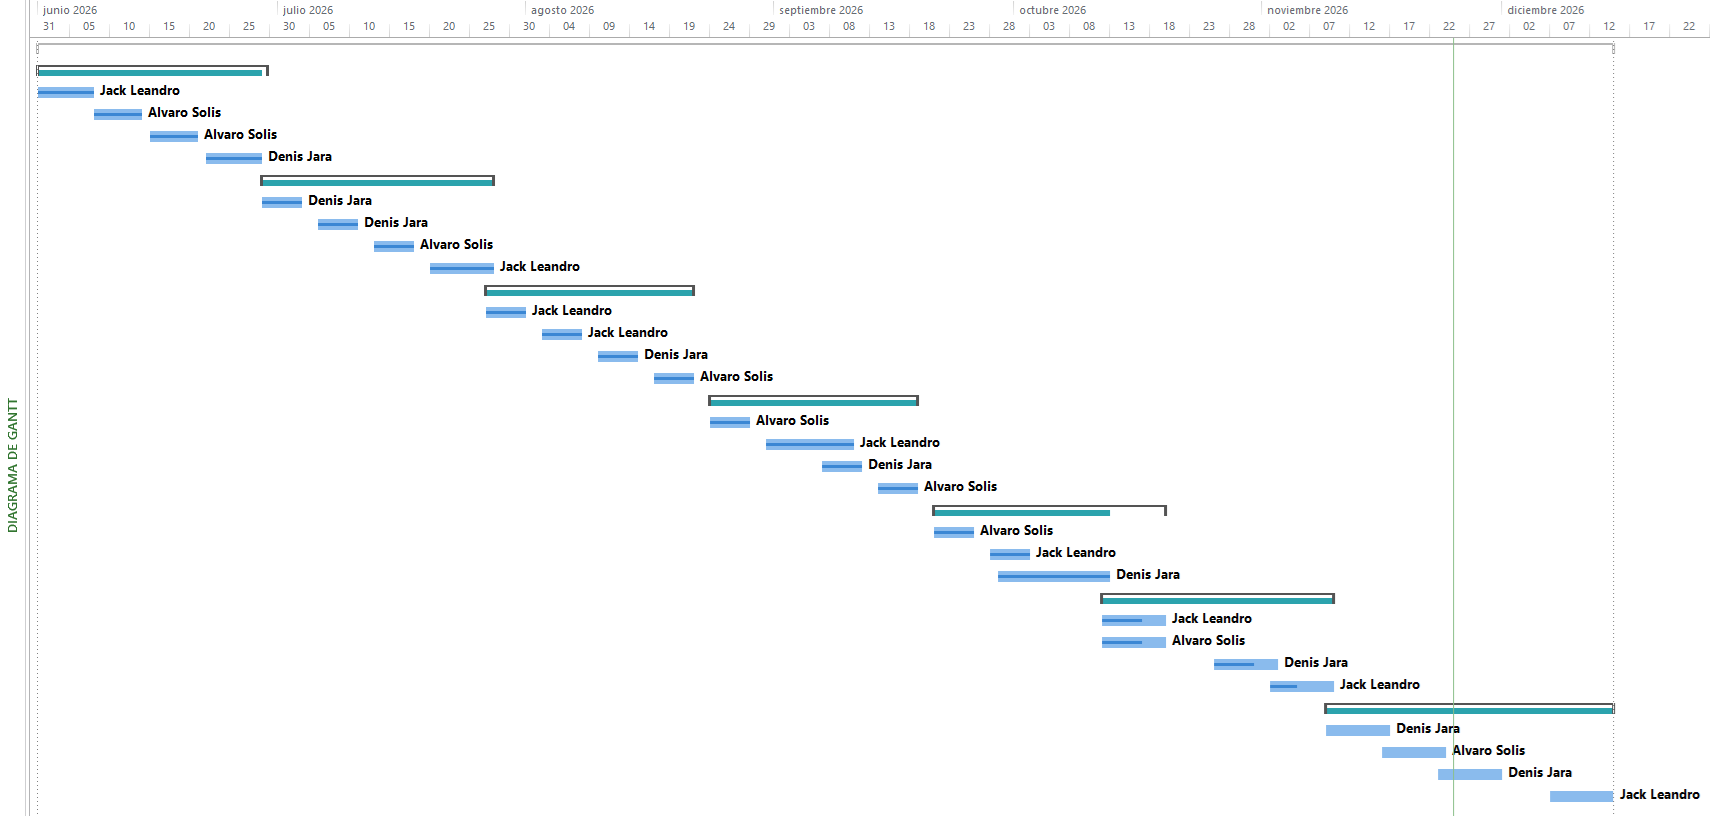
\includegraphics[width=0.98\textwidth, trim=0 0 0 0, clip]{Cronograma-Proyecto-2.png}

\vspace{-0.4em}
{\small \textit{Nota.} Elaboración propia basada en la planificación del sistema Help-Desk centralizado en Microsoft Project. Segunda parte del cronograma.}

\end{figure}

Como se observa en la figura, el porcentaje de completado de las tareas está representado mediante una escala de colores en la columna correspondiente. El \textbf{color verde oscuro} indica las fases y tareas concluidas al 100\% (valor máximo), correspondientes a la arquitectura base, desarrollo del backend y la mayor parte del frontend. El \textbf{color amarillo} denota una tarea en curso con un avance parcial del 66\% (correspondiente a pantallas de inventario ITAM, tickets, chat y dashboard). Por último, el \textbf{color rojo} señala las actividades pendientes con un avance del 0\%, vinculadas a la fase final de control de calidad, exportación PDF y despliegue en producción.

\newpage

\section{Aspecto limitante para la implementación de la mejora}
Durante el proceso de implantación y puesta en marcha de la solución tecnológica centralizada, se han identificado diversos factores limitantes de carácter técnico, operativo y organizacional que podrían influir en la adopción del sistema. Estos aspectos se clasifican y detallan a continuación según los actores involucrados:

\begin{itemize}
\item \textbf{Limitaciones asociadas a la empresa (J\&P Periféricos S.A.C. - JYP) y su infraestructura tecnológica:}
\begin{itemize}
\item \textbf{Dependencia de la infraestructura de red y servidores:} Al operar bajo una arquitectura web modular con comunicaciones en tiempo real mediante WebSockets (para notificaciones y el chat del ticket) y transacciones síncronas a través de Prisma ORM sobre MySQL, cualquier interrupción en el suministro eléctrico o caída del servidor en producción afecta de manera directa la continuidad operativa de la plataforma de ayuda.
\item \textbf{Validación y carga inicial masiva de datos:} La precisión del módulo de inventario (ITAM) depende críticamente de la calidad de los datos iniciales migrados. Errores humanos durante la importación masiva mediante plantillas de Excel o en el registro de series y componentes pueden generar inconsistencias transitorias en las hojas de vida de los equipos.
\end{itemize}

\item \textbf{Limitaciones asociadas al personal de soporte técnico:}
\begin{itemize}
    \item \textbf{Curva de adaptación a los flujos automatizados:} El personal técnico debe habituarse rigurosamente al motor de asignación automática por zonas, al uso de estados transaccionales (pendientes, en camino, en progreso, espera de repuestos) y a los bloqueos de concurrencia (\textit{SoftLock}), lo cual demanda un periodo inicial de supervisión para evitar la manipulación incorrecta de los estados del ticket.

\newpage

    \item \textbf{Cuellos de botella en la atención in-situ:} La gestión de citas presenciales está condicionada por la disponibilidad horaria de los técnicos de campo y la distribución geográfica de las sucursales. Ante incidencias masivas concurrentes, la capacidad de respuesta física puede verse saturada temporalmente.
\end{itemize}

\item \textbf{Limitaciones asociadas a los clientes y usuarios (Empresa, Sucursal y Trabajadores):}
\begin{itemize}
    \item \textbf{Resistencia al cambio frente a canales informales:} Existe una tendencia arraigada en los usuarios finales de recurrir a canales de comunicación informales y directos (llamadas telefónicas o mensajes de WhatsApp) en lugar de registrar la incidencia de manera formal en el portal web y aguardar su código PIN de seguimiento.
    \item \textbf{Brecha digital y precisión en el reporte de incidencias:} La correcta categorización del problema (hardware o software) y la selección adecuada del activo asignado dependen de la destreza digital del trabajador; descripciones imprecisas en la solicitud inicial pueden retrasar el diagnóstico remoto por parte del equipo técnico.
\end{itemize}

\end{itemize}
\cleardoublepage

\chapter[CAPÍTULO V]{COSTO DE IMPLEMENTACIÓN DE MEJORA / INNOVACIÓN / CREATIVIDAD}

\section{Costo de Materiales}

Este rubro reúne los servicios digitales, infraestructura en la nube y herramientas indispensables considerados para poner en funcionamiento y asegurar el acceso público al sistema HelpDesk. A continuación se identifican los servicios registrados, su nombre y sus respectivos costos en soles. Para facilitar la comparación, los importes en dólares se expresan utilizando el tipo de cambio referencial de S/ 3.42 por dólar estadounidense.

\vspace{0.3cm}

\begingroup
\small
\renewcommand{\arraystretch}{1.25}
\begin{longtable}{@{} p{4.5cm} p{2.2cm} p{3.8cm} p{2.2cm} p{2.2cm} @{}}
\caption{{Costo de materiales y servicios digitales}} \label{tab:costo_materiales} \\
\toprule
\textbf{Concepto / Servicio} & \textbf{Nombre} & \textbf{Costo (S/.)} & \textbf{Dólar \$} \\
\midrule
\endfirsthead

\multicolumn{5}{@{}l}{\textbf{Tabla \ref{tab:costo_materiales}} \textit{(Continuación)}} \\[0.4em]
\toprule
\textbf{Concepto / Servicio}  & \textbf{Nombre} & \textbf{Costo (S/.)} & \textbf{Dólar \$} \\
\midrule
\endhead

\midrule
\multicolumn{5}{r}{\textit{Continúa en la siguiente página\dots}} \\
\endfoot

\bottomrule
\multicolumn{5}{@{}p{\textwidth}}{\small \textit{Nota.} Detalle de los servicios digitales y de infraestructura requeridos para la puesta en marcha y despliegue del sistema web. Los importes en dólares se calcularon a partir de los costos en soles, utilizando un tipo de cambio referencial de S/ 3.42 por dólar estadounidense.} \\
\endlastfoot

Base de datos & MySQL / MongoDB / Prisma & S/ 00.00 & \$ 00.00 \\
Servidor Hosting & Servidor Interno J\&P & S/ 0.00 & \$ 0.00 \\
Servidor Local & Memoria Ram Fury Beast 16 GB, 3200 MHz  & S/ 455 & \$ 131.40 \\
Certificado SSL (HTTPS) & PositiveSSL & S/ 88.00 & \$ 25.41 \\
\textbf{Total} & & \textbf{S/ 543.00} & \textbf{\$ 156.81} \\
\end{longtable}
\endgroup

Los servicios digitales considerados comprenden la base de datos en la nube (MySQL / MongoDB / Prisma), el servidor de alojamiento (\textit{hosting}) para el despliegue del backend y frontend, y el registro del dominio web institucional, garantizando la disponibilidad y seguridad de la plataforma para los usuarios y técnicos de J\&P Periféricos S.A.C.

\section{Costo de Mano de Obra}

Los servicios digitales considerados comprenden la base de datos en la nube (MySQL / MongoDB / Prisma), el servidor de alojamiento (\textit{hosting}) para el despliegue del backend y frontend, y el registro del dominio web institucional, garantizando la disponibilidad y seguridad de la plataforma para los usuarios y técnicos de J\&P Periféricos S.A.C. Los importes en dólares se expresan utilizando el tipo de cambio referencial de S/ 3.42 por dólar estadounidense.
\vspace{0.3cm}

\begingroup
\small
\renewcommand{\arraystretch}{1.25}
\begin{longtable}{@{} p{3.9cm} p{1.6cm} p{2.2cm} p{2.5cm} p{2.2cm} p{1.8cm} @{}}
\caption{{Costo de mano de obra del equipo de desarrollo}} \label{tab:costo_mano_obra} \\
\toprule
\textbf{Actividad} & \textbf{Cantidad} & \textbf{Días laborables} & \textbf{Costo unitario (S/.)} & \textbf{Total (S/.)} & \textbf{Dólar \$} \\
\midrule
\endfirsthead

\multicolumn{6}{@{}l}{\textbf{Tabla \ref{tab:costo_mano_obra}} \textit{(Continuación)}} \\[0.4em]
\toprule
\textbf{Actividad} & \textbf{Cantidad} & \textbf{Días laborables} & \textbf{Costo unitario (S/.)} & \textbf{Total (S/.)} & \textbf{Dólar \$} \\
\midrule
\endhead

\midrule
\multicolumn{6}{r}{\textit{Continúa en la siguiente página\dots}} \\
\endfoot

\bottomrule
\multicolumn{6}{@{}p{\textwidth}}{\small \textit{Nota.} Distribución de jornadas (149 días correspondientes a los Sprints 0--5) y costos de mano de obra del equipo de desarrollo. La conversión a dólares se realizó con el tipo de cambio referencial de S/ 3.42.} \\
\endlastfoot

Desarrollador & 1 & 149 & S/ 30.00 & S/ 4,470.00 & \$ 1,307.02 \\
Desarrollador & 1 & 149 & S/ 30.00 & S/ 4,470.00 & \$ 1,307.02 \\
Desarrollador & 1 & 149 & S/ 30.00 & S/ 4,470.00 & \$ 1,307.02 \\
\textbf{Total} & & & & \textbf{S/ 13,410.00} & \textbf{\$ 3,921.05} \\
\end{longtable}
\endgroup
La tarifa diaria de S/ 30.00 por mano de obra considera el perfil junior de los desarrolladores según la clasificación del MTPE(Ministerio de Trabajo y Promoción del Empleo), ajustada a los rangos de mercado para desarrolladores en Lima, Perú, y refleja una tarifa colaborativa institucional por debajo del valor de mercado para fomentar la innovación en J\&P Periféricos S.A.C.; Además, según el Anuario Estadístico MTPE 2024, la remuneración en el sector formal privado promedia S/ 2,898 mensuales, y para jóvenes (18-29 años) alcanza S/ 1,905, lo que respalda que la tarifa de S/ 30.00/día representa un costo racional y ajustado para un perfil junior de desarrollo de software.
\newpage

\section{Costo de Máquinas, Herramientas y Equipos}
\subsection{El Costo de Depreciación de herramientas}

Para desarrollar el sistema HelpDesk, los integrantes del equipo utilizaron sus propias computadoras. Se utiliza la formula: Valor inicial / vida útil en años para calcular el valor residual.

\vspace{0.3cm}

\begingroup
\small
\renewcommand{\arraystretch}{1.25}
\begin{longtable}{@{} p{3.5cm} p{10.9cm} @{}}
\caption{{Equipo de cómputo del primer desarrollador}} \label{tab:equipo_dev1} \\
\toprule
\textbf{Nombre} & \textbf{Descripción} \\
\midrule
\endfirsthead

\multicolumn{2}{@{}l}{\textbf{Tabla \ref{tab:equipo_dev1}} \textit{(Continuación)}} \\[0.4em]
\toprule
\textbf{Nombre} & \textbf{Descripción} \\
\midrule
\endhead

\midrule
\multicolumn{2}{r}{\textit{Continúa en la siguiente página\dots}} \\
\endfoot

\bottomrule
\multicolumn{2}{@{}p{\textwidth}}{\small \textit{Nota.} Computadora utilizada como equipo principal de trabajo por uno de los desarrolladores.} \\
\endlastfoot

Característica de la PC: & AMD Ryzen 5 8600G w/ Radeon 760M Graphics (4.35 GHz) - 32.0 GB RAM \\
Valor inicial: & S/ 2,800.00 \\
Vida útil en años: & 5 años \\
Valor residual: & S/ 560 \\
\end{longtable}
\endgroup

\vspace{0.3cm}

\begingroup
\small
\renewcommand{\arraystretch}{1.25}
\begin{longtable}{@{} p{3.5cm} p{10.9cm} @{}}
\caption{{Equipo de cómputo del segundo desarrollador}} \label{tab:equipo_dev2} \\
\toprule
\textbf{Nombre} & \textbf{Descripción} \\
\midrule
\endfirsthead

\multicolumn{2}{@{}l}{\textbf{Tabla \ref{tab:equipo_dev2}} \textit{(Continuación)}} \\[0.4em]
\toprule
\textbf{Nombre} & \textbf{Descripción} \\
\midrule
\endhead

\midrule
\multicolumn{2}{r}{\textit{Continúa en la siguiente página\dots}} \\
\endfoot

\bottomrule
\multicolumn{2}{@{}p{\textwidth}}{\small \textit{Nota.} Computadora utilizada como equipo principal de trabajo por uno de los desarrolladores.} \\
\endlastfoot

Característica de la PC: & AMD Ryzen 3 2200G - 8.0 GB RAM - NVIDIA GeForce 210 - 224 GB SSD \\
Valor inicial: & S/ 1,600.00 \\
Vida Util en años: & 5 años \\
Valor residual: & S/ 320 \\
\end{longtable}
\endgroup

\vspace{0.3cm}

\begingroup
\small
\renewcommand{\arraystretch}{1.25}
\begin{longtable}{@{} p{3.5cm} p{10.9cm} @{}}
\caption{{Equipo de cómputo del tercer desarrollador}} \label{tab:equipo_dev3} \\
\toprule
\textbf{Nombre} & \textbf{Descripción} \\
\midrule
\endfirsthead

\multicolumn{2}{@{}l}{\textbf{Tabla \ref{tab:equipo_dev3}} \textit{(Continuación)}} \\[0.4em]
\toprule
\textbf{Nombre} & \textbf{Descripción} \\
\midrule
\endhead

\midrule
\multicolumn{2}{r}{\textit{Continúa en la siguiente página\dots}} \\
\endfoot

\bottomrule
\multicolumn{2}{@{}p{\textwidth}}{\small \textit{Nota.} Computadora utilizada como equipo principal de trabajo por uno de los desarrolladores.} \\
\endlastfoot

Característica de la PC: & AMD Ryzen 7 5700G - 20.0 GB RAM - 424 GB Almacenamiento \\
Valor inicial: & S/ 2,600.00 \\
Vida Util en años: & 5 años \\
Valor residual: & S/ 520 \\
\end{longtable}
\endgroup

Para estimar el costo asociado al uso de las computadoras se aplica el método de depreciación lineal. Este método distribuye el valor depreciable del equipo en partes iguales a lo largo de su vida útil.

\begin{equation}
\text{Depreciación} =
\frac{\text{Valor inicial} - \text{Valor residual}}{\text{Vida útil en años}}
\end{equation}

\vspace{0.3cm}

\begingroup
\small
\renewcommand{\arraystretch}{1.25}
\begin{longtable}{@{} p{4.5cm} p{2.2cm} r c r c l @{}}
\caption{{Depreciación de los equipos de cómputo de cada desarrollador}} \label{tab:depreciacion_equipos} \\
\toprule
\textbf{Nombre} & \multicolumn{6}{l}{\textbf{Cálculo}} \\
\midrule
\endfirsthead

\multicolumn{7}{@{}l}{\textbf{Tabla \ref{tab:depreciacion_equipos}} \textit{(Continuación)}} \\[0.4em]
\toprule
\textbf{Nombre} & \multicolumn{6}{l}{\textbf{Cálculo}} \\
\midrule
\endhead

\midrule
\multicolumn{7}{r}{\textit{Continúa en la siguiente página\dots}} \\
\endfoot

\bottomrule
\multicolumn{7}{@{}p{\textwidth}}{\small \textit{Nota.} Cálculo realizado mediante el método de depreciación lineal, considerando el valor depreciable (Valor inicial menos valor residual) entre los 5 años de vida útil.} \\
\endlastfoot

Computadora del desarrollador 1 & Depreciación: & S/ 448.00 & = & S/ 2,240.00 & / & 5 años \\
Computadora del desarrollador 2 & Depreciación: & S/ 256.00 & = & S/ 1,280.00 & / & 5 años \\
Computadora del desarrollador 3 & Depreciación: & S/ 416.00 & = & S/ 2,080.00 & / & 5 años \\
\end{longtable}
\endgroup

De acuerdo con los cálculos anteriores, la depreciación acumulada de las tres computadoras principales asciende a \textbf{S/ 280.00} durante los tres meses de desarrollo (prorrateado a S/ 93.33 mensuales o S/ 1,120.00 anuales en conjunto).

\vspace{0.3cm}

\begingroup
\small
\renewcommand{\arraystretch}{1.25}
\begin{longtable}{@{} p{3.5cm} r c r c r @{}}
\caption{{Depreciación anual del equipo de cómputo del Desarrollador 1}} \label{tab:deprec_dev1_anios} \\
\toprule
\textbf{Valor} & \textbf{Valor residual} & & \textbf{Depreciación} & & \textbf{Resultado} \\
\midrule
\endfirsthead

\multicolumn{6}{@{}l}{\textbf{Tabla \ref{tab:deprec_dev1_anios}} \textit{(Continuación)}} \\[0.4em]
\toprule
\textbf{Valor} & \textbf{Valor residual} & & \textbf{Depreciación} & & \textbf{Resultado} \\
\midrule
\endhead

\midrule
\multicolumn{6}{r}{\textit{Continúa en la siguiente página\dots}} \\
\endfoot

\bottomrule
\multicolumn{6}{@{}p{\textwidth}}{\small \textit{Nota.} Muestra el proceso de depreciación lineal anual para el primer equipo hasta alcanzar su valor residual.} \\
\endlastfoot

1 año Valor: & S/ 2,240.00 & & & & \\
2 año Valor: & S/ 2,240.00 & - & S/ 448.00 & = & S/ 1,792.00 \\
3 año Valor: & S/ 1,792.00 & - & S/ 448.00 & = & S/ 1,344.00 \\
4 año Valor: & S/ 1,344.00 & - & S/ 448.00 & = & S/ 896.00 \\
5 año Valor: & S/ 896.00 & - & S/ 448.00 & = & S/ 448.00 \\
- & S/ 448.00 & - & S/ 448.00 & = & S/ 0.00 \\
\end{longtable}
\endgroup

\vspace{0.3cm}

\begingroup
\small
\renewcommand{\arraystretch}{1.25}
\begin{longtable}{@{} p{3.5cm} r c r c r @{}}
\caption{{Depreciación anual del equipo de cómputo del Desarrollador 2}} \label{tab:deprec_dev2_anios} \\
\toprule
\textbf{Valor} & \textbf{Valor residual} & & \textbf{Depreciación} & & \textbf{Resultado} \\
\midrule
\endfirsthead

\multicolumn{6}{@{}l}{\textbf{Tabla \ref{tab:deprec_dev2_anios}} \textit{(Continuación)}} \\[0.4em]
\toprule
\textbf{Valor} & \textbf{Valor residual} & & \textbf{Depreciación} & & \textbf{Resultado} \\
\midrule
\endhead

\midrule
\multicolumn{6}{r}{\textit{Continúa en la siguiente página\dots}} \\
\endfoot

\bottomrule
\multicolumn{6}{@{}p{\textwidth}}{\small \textit{Nota.} Muestra el proceso de depreciación lineal anual para el segundo equipo hasta alcanzar su valor residual.} \\
\endlastfoot

1 año Valor: & S/ 1,280.00 & & & & \\
2 año Valor: & S/ 1,280.00 & - & S/ 256.00 & = & S/ 1,024.00 \\
3 año Valor: & S/ 1,024.00 & - & S/ 256.00 & = & S/ 768.00 \\
4 año Valor: & S/ 768.00 & - & S/ 256.00 & = & S/ 512.00 \\
5 año Valor: & S/ 512.00 & - & S/ 256.00 & = & S/ 256.00 \\
- & S/ 256.00 & - & S/ 256.00 & = & S/ 0.00 \\
\end{longtable}
\endgroup

\vspace{0.3cm}

\begingroup
\small
\renewcommand{\arraystretch}{1.25}
\begin{longtable}{@{} p{3.5cm} r c r c r @{}}
\caption{{Depreciación anual del equipo de cómputo del Desarrollador 3}} \label{tab:deprec_dev3_anios} \\
\toprule
\textbf{Valor} & \textbf{Valor residual} & & \textbf{Depreciación} & & \textbf{Resultado} \\
\midrule
\endfirsthead

\multicolumn{6}{@{}l}{\textbf{Tabla \ref{tab:deprec_dev3_anios}} \textit{(Continuación)}} \\[0.4em]
\toprule
\textbf{Valor} & \textbf{Valor residual} & & \textbf{Depreciación} & & \textbf{Resultado} \\
\midrule
\endhead

\midrule
\multicolumn{6}{r}{\textit{Continúa en la siguiente página\dots}} \\
\endfoot

\bottomrule
\multicolumn{6}{@{}p{\textwidth}}{\small \textit{Nota.} Muestra el proceso de depreciación lineal anual para el tercer equipo hasta alcanzar su valor residual.} \\
\endlastfoot

1 año Valor: & S/ 2,080.00 & & & & \\
2 año Valor: & S/ 2,080.00 & - & S/ 416.00 & = & S/ 1,664.00 \\
3 año Valor: & S/ 1,664.00 & - & S/ 416.00 & = & S/ 1,248.00 \\
4 año Valor: & S/ 1,248.00 & - & S/ 416.00 & = & S/ 832.00 \\
5 año Valor: & S/ 832.00 & - & S/ 416.00 & = & S/ 416.00 \\
- & S/ 416.00 & - & S/ 416.00 & = & S/ 0.00 \\
\end{longtable}
\endgroup

\subsection{El Costo de Licencia de Software y Depreciación}

Para el adecuado funcionamiento del equipo de desarrollo, se adquirieron licenciamientos de software y recursos de equipamiento complementario. Además de las computadoras principales utilizadas por los desarrolladores, se consideran herramientas esenciales y de nivel profesional para la creación, pruebas integrales, despliegue continuo y mantenimiento del sistema HelpDesk. El uso de licencias oficiales y frameworks de desarrollo garantiza entornos de trabajo estables, seguros y compatibles con los estándares de la industria de software, permitiendo una integración continua y despliegues confiables en el entorno de producción. Asimismo, se contempla la depreciación proporcional de computadoras adicionales de soporte empleadas durante el ciclo de innovación, las cuales complementan el parque informático principal y aseguran que el equipo de trabajo cuente con recursos hardware suficientes para ejecutar los procesos de desarrollo, pruebas de carga y validación de funcionalidades sin interferir en el uso cotidiano de los equipos principales. Estos recursos de licenciamiento y equipamiento son indispensables para mantener la continuidad del equipo de trabajo, garantizar la integración de los frameworks de trabajo colaborativo y cumplir con los plazos del proyecto de innovación, ya que la ausencia de herramientas profesionales y equipos de soporte adecuados implicaría retrasos significativos en los tiempos de desarrollo, pruebas y validación del sistema. La \textbf{Tabla 30} detalla los importes correspondientes a dichos elementos, considerando licencias de herramientas de desarrollo y la depreciación proporcional de computadoras adicionales de soporte empleadas durante el ciclo de innovación, las cuales son indispensables para mantener la continuidad del equipo de trabajo y la integración de los frameworks de trabajo colaborativo.

\begingroup
\small
\renewcommand{\arraystretch}{1.25}
\begin{longtable}{@{} p{5.0cm} p{2.0cm} p{3.2cm} p{2.5cm} p{1.7cm} @{}}
\caption{{Costo de licenciamiento de software y equipamiento adicional}} \label{tab:licenciamiento_adicional} \\
\toprule
\textbf{Descripción} & \textbf{Cantidad} & \textbf{Costo unitario (S/.)} & \textbf{Total (S/.)} & \textbf{Dólar \$} \\
\midrule
\endfirsthead

\multicolumn{5}{@{}l}{\textbf{Tabla \ref{tab:licenciamiento_adicional}} \textit{(Continuación)}} \\[0.4em]
\toprule
\textbf{Descripción} & \textbf{Cantidad} & \textbf{Costo unitario (S/.)} & \textbf{Total (S/.)} & \textbf{Dólar \$} \\
\midrule
\endhead

\midrule
\multicolumn{5}{r}{\textit{Continúa en la siguiente página\dots}} \\
\endfoot

\bottomrule
\multicolumn{5}{@{}p{\textwidth}}{\small \textit{Nota.} Importes de licenciamiento y equipamiento complementario. Conversión a dólares utilizando un tipo de cambio referencial de S/ 3.42.} \\
\endlastfoot
Visual Studio Code & 7 & S/ 00.00 & S/ 00.00 & \$ 00.00 \\
Docker Compose & 2 & S/ 00.00 & S/ 00.00 & \$ 00.00 \\
Frameworks(NestJs, Vite 8.2 + React) & 7 & S/ 00.00 & S/ 00.00 & \$ 00.00 \\
Depreciación PC adicional 1 & 3 & S/ 395.83 & S/ 1,187.49 & \$ 342.98 \\
Depreciación PC adicional 2 & 2 & S/ 450.00 & S/ 900.00 & \$ 259.95 \\
Depreciación PC adicional 3 & 2 & S/ 410.00 & S/ 820.00 & \$ 236.84 \\
\textbf{Total} & & & \textbf{S/ 2,907.49} & \textbf{\$ 839.77} \\
\end{longtable}
\endgroup

\section{Otros costos de Implementación de mejora}
\subsection{El Costo de Servicio de consumo de Luz}

Para estimar el consumo eléctrico se considera un promedio de 230 kWh mensuales y una tarifa de S/ 0.65 por kWh.

\begin{equation}
\text{Costo mensual} = 230\text{ kWh} \times \text{S/ 0.65 por kWh} = \text{S/ 149.50}
\end{equation}

\vspace{0.3cm}

\begingroup
\small
\renewcommand{\arraystretch}{1.25}
\begin{longtable}{@{} p{5.5cm} p{2.5cm} p{2.5cm} p{2.0cm} p{1.9cm} @{}}
\caption{{Cálculo del consumo de energía eléctrica durante el proyecto}} \label{tab:consumo_electrico} \\
\toprule
\textbf{Concepto} & \textbf{Consumo} & \textbf{Tarifa} & \textbf{Duración} & \textbf{Total (S/.)} \\
\midrule
\endfirsthead

\multicolumn{5}{@{}l}{\textbf{Tabla \ref{tab:consumo_electrico}} \textit{(Continuación)}} \\[0.4em]
\toprule
\textbf{Concepto} & \textbf{Consumo} & \textbf{Tarifa} & \textbf{Duración} & \textbf{Total (S/.)} \\
\midrule
\endhead

\midrule
\multicolumn{5}{r}{\textit{Continúa en la siguiente página\dots}} \\
\endfoot

\bottomrule
\multicolumn{5}{@{}p{\textwidth}}{\small \textit{Nota.} Estimación del consumo eléctrico asignado al período de desarrollo en J\&P Periféricos S.A.C.} \\
\endlastfoot

Consumo de energía eléctrica & 230 kWh/mes & S/ 0.65/kWh & 3 meses & 448.50 \\
\textbf{Costo total} & & & \textbf{3 meses} & \textbf{448.50} \\
\end{longtable}
\endgroup

\subsection{Lista de gastos adicionales}

Se incluye también el servicio de internet Movistar de 400 Mbps con un costo mensual de S/ 89.90 durante tres meses.

\vspace{0.3cm}

\begingroup
\small
\renewcommand{\arraystretch}{1.25}
\begin{longtable}{@{} p{5.0cm} p{1.8cm} p{3.2cm} p{2.5cm} p{1.9cm} @{}}
\caption{{Gastos de operación y servicios utilizados durante el proyecto}} \label{tab:gastos_operacion} \\
\toprule
\textbf{Descripción} & \textbf{Meses} & \textbf{Precio mensual (S/.)} & \textbf{Total (S/.)} & \textbf{Dólar \$} \\
\midrule
\endfirsthead

\multicolumn{5}{@{}l}{\textbf{Tabla \ref{tab:gastos_operacion}} \textit{(Continuación)}} \\[0.4em]
\toprule
\textbf{Descripción} & \textbf{Meses} & \textbf{Precio mensual (S/.)} & \textbf{Total (S/.)} & \textbf{Dólar \$} \\
\midrule
\endhead

\midrule
\multicolumn{5}{r}{\textit{Continúa en la siguiente página\dots}} \\
\endfoot

\bottomrule
\multicolumn{5}{@{}p{\textwidth}}{\small \textit{Nota.} Gastos operativos de energía e internet por tres meses. Conversión a dólares utilizando el tipo de cambio referencial de S/ 3.42.} \\
\endlastfoot

Servicio de energía eléctrica & 3 & 149.50 & 448.50 & \$ 131.14 \\
Servicio de internet (Movistar 400 Mbps) & 3 & 89.90 & 269.70 & \$ 78.86 \\
\textbf{Total} & & & \textbf{718.20} & \textbf{\$ 210.00} \\
\end{longtable}
\endgroup

\section{Costo total de la Implementación de Mejora / Innovación / Creatividad}

A continuación se consolidan todos los rubros en el presupuesto general de la implementación del sistema.

\vspace{0.3cm}

\begingroup
\small
\renewcommand{\arraystretch}{1.25}
\begin{longtable}{@{} p{9.4cm} p{2.5cm} p{2.5cm} @{}}
\caption{{Presupuesto general de implementación del sistema HelpDesk}} \label{tab:presupuesto_general} \\
\toprule
\textbf{Descripción} & \textbf{Total (S/.)} & \textbf{Dólar \$} \\
\midrule
\endfirsthead

\multicolumn{3}{@{}l}{\textbf{Tabla \ref{tab:presupuesto_general}} \textit{(Continuación)}} \\[0.4em]
\toprule
\textbf{Descripción} & \textbf{Total (S/.)} & \textbf{Dólar \$} \\
\midrule
\endhead

\midrule
\multicolumn{3}{r}{\textit{Continúa en la siguiente página\dots}} \\
\endfoot

\bottomrule
\multicolumn{3}{@{}p{\textwidth}}{\small \textit{Nota.} Presupuesto consolidado para la implementación del sistema utilizando un tipo de cambio referencial de S/ 3.42.} \\
\endlastfoot

Costo de materiales y servicios digitales & 543.00 & 158.77 \\
Costo de mano de obra & 13,410.00 & 3,921.05 \\
Costo de máquinas, herramientas y equipos & 3,582.99 & 1,047.66 \\
Otros costos de operación y conectividad & 718.20 & 210.00 \\
\textbf{Total general de implementación} & \textbf{18,254.19} & \textbf{5,337.48} \\
\end{longtable}
\endgroup

\vspace{0.2cm}

La inversión total de \textbf{S/ 18,254.19} (US\$ 5,337.48) en la implementación del sistema \textit{HelpDesk} refleja una estructura financiera concentrada en un 73.5\% en mano de obra especializada, un 19.6\% en máquinas, herramientas y equipos, un 3.9\% en otros costos de operación y conectividad, y un 3.0\% en materiales y servicios digitales. Cada rubro ha sido considerado bajo criterios de eficiencia presupuestaria, aprovechamiento de recursos internos y operatividad tecnológica para J\&P Periféricos S.A.C.
\cleardoublepage

\chapter[CAPÍTULO VI]{EVALUACIÓN TÉCNICA Y ECONÓMICA DE LA MEJORA / INNOVACIÓN / CREATIVIDAD}

\section{Beneficio técnico y/o económico esperado de la mejora / Innovación / Creatividad}

La implementación del \textbf{Sistema Web Help-Desk Centralizado} en \textbf{J\&P Periféricos S.A.C.} está orientada a resolver el problema principal de desorganización y falta de trazabilidad en la gestión de incidencias y el control del inventario informático multinivel (empresa cliente, sucursal, área y trabajador) para clientes corporativos externos. Desde la ingeniería de software (arquitectura hexagonal en NestJS con TypeScript, Prisma ORM sobre MySQL, MongoDB para historial de chats, Redis Pub/Sub y WebSockets en tiempo real, y \textit{frontend} modular en Vite + React con \textit{shadcn/ui}) y las prácticas de \textbf{ITSM / ITIL v4 e ITAM}, los beneficios esperados se estructuran en dimensiones técnicas y económicas:

\begin{itemize}
    \item \textbf{Centralización y trazabilidad integral de solicitudes (SPOC):} Reemplaza el ingreso informal por llamadas telefónicas y mensajes de WhatsApp sin registro (Causa CA2) mediante una consola web centralizada donde cada incidencia se registra con un código PIN único, máquina de estados auditable y registro de eventos críticos (\texttt{auditoria\_eventos}), asegurando que no se pierdan solicitudes ni se dupliquen atenciones.
    \item \textbf{Agilidad y exactitud en la gestión de activos TI (ITAM):} Sustituye las planillas dispersas y desactualizadas de Excel (Causa CA1) por un expediente digital multinivel con hoja de vida técnica por equipo, trazabilidad de componentes físicos instalados/reemplazados (\texttt{hardware} y \texttt{registro\_hardware}) y bóveda de licencias de software (\texttt{software} y \texttt{software\_equipos}), reduciendo el tiempo de búsqueda previa al diagnóstico.
    \item \textbf{Optimización de visitas técnicas \textit{in-situ} y control de concurrencia:} Incorpora un motor de autoasignación por zona geográfica (\texttt{tecnicos\_zonas}), evaluación de carga laboral, agrupación de hasta tres atenciones en una misma sucursal y franja horaria, y bloqueos temporales (\textit{soft\_locks}), reduciendo los cruces de agenda (Causa CA3), los traslados duplicados y los tiempos muertos en ruta.
    \item \textbf{Estandarización del escalamiento y validación digital de planes y SLA:} Formaliza el flujo de derivación desde soporte remoto hacia soporte \textit{in-situ} con registro del motivo y antecedentes del ticket (Causa CA4), al tiempo que centraliza los planes de soporte (vigencia, servicios incluidos, precios y límite de equipos) para evitar atenciones fuera de cobertura y mejorar el cumplimiento de los Acuerdos de Nivel de Servicio (Causa CA5).
    \item \textbf{Analítica continua y soporte a la decisión gerencial:} Automatiza el cálculo y visualización de indicadores clave de rendimiento (\textbf{MTTA, MTTR, FCR y CSAT}) y métricas operativas en el \textit{dashboard} (Causas CA6 y CA7), eliminando la consolidación manual de reportes a fin de mes y brindando información objetiva para evaluar la calidad del servicio.
    \item \textbf{Retención y confianza de clientes corporativos:} Provee transparencia sobre el estado de las incidencias, el historial de intervenciones y el cumplimiento de tiempos pactados, fortaleciendo la relación comercial de J\&P Periféricos S.A.C. con sus empresas clientes.
\end{itemize}

\section{Relación de beneficio / costo}

La evaluación económica contrasta la \textbf{inversión total de implementación} cuantificada en el Capítulo V (\textbf{S/ 18,254.19} o \textbf{US\$ 5,337.48} al tipo de cambio referencial de S/ 3.42) frente a los \textbf{ahorros operativos} derivados de mitigar las ineficiencias diagnosticadas en el Capítulo III, aplicando el indicador de relación \textbf{Beneficio/Costo (B/C)} y el \textbf{período de recuperación de la inversión (\textit{Payback})}.

\subsection{Identificación de la Pérdida Económica}

A partir del diagnóstico cuantitativo del Capítulo III ---basado en el registro empírico de 5 meses (mayo a septiembre de 2026, con un total de 395 atenciones, una plantilla operativa de 3 técnicos y un costo hora-hombre de \textbf{S/ 25.00})--- se identifican las pérdidas económicas directas asociadas a las tres causas principales priorizadas en el análisis de Pareto, cuyo consolidado mensual y anual se detalla en la Tabla \ref{tab:perdida_economica_cap6}:

\begin{enumerate}
    \item \textbf{Causa CA1 --- Búsqueda manual de datos de equipos en archivos Excel desactualizados:} Se registraron 103 atenciones con demora en 5 meses (26\% promedio), con una paralización estimada de 25 minutos por incidencia. El impacto en los 5 meses asciende a \textbf{S/ 1,072.90}, equivalente a un promedio mensual de \textbf{S/ 214.58} y una proyección anual (12 meses) de \textbf{S/ 2,574.96}.
    \item \textbf{Causa CA2 --- Recepción y comunicación por canales informales (WhatsApp/llamadas) sin registro:} Se registraron 149 solicitudes informales en 5 meses (38\% promedio), con un tiempo improductivo promedio de 30 minutos por solicitud. El impacto en los 5 meses asciende a \textbf{S/ 1,862.50}, equivalente a un promedio mensual de \textbf{S/ 372.50} y una proyección anual (12 meses) de \textbf{S/ 4,470.00}.
    \item \textbf{Causa CA3 --- Descoordinación y reubicación de horarios por cruces en visitas \textit{in-situ}:} Se registraron 81 visitas presenciales afectadas por cruces de agenda y reprogramaciones en 5 meses (20\% promedio), con un tiempo muerto promedio de 20 minutos y sobrecostos operativos de traslado. El impacto en los 5 meses asciende a \textbf{S/ 675.00}, equivalente a un promedio mensual de \textbf{S/ 135.00} y una proyección anual (12 meses) de \textbf{S/ 1,620.00}.
\end{enumerate}

\begin{table}[H]
\centering
\small
\renewcommand{\arraystretch}{1.25}
\caption{Consolidado de Pérdidas Económicas Operativas Identificadas (Situación Actual)}
\label{tab:perdida_economica_cap6}
\begin{tabular}{@{} >{\raggedright\arraybackslash}p{1.2cm} >{\raggedright\arraybackslash}p{5.2cm} >{\raggedright\arraybackslash}p{3.0cm} >{\raggedleft\arraybackslash}p{2.0cm} >{\raggedleft\arraybackslash}p{2.2cm} >{\raggedleft\arraybackslash}p{1.6cm} @{}}
\toprule
\textbf{Código} & \textbf{Causa Raíz Principal} & \textbf{Tipo de Pérdida} & \textbf{Estimación Mensual (S/.)} & \textbf{Proyección Anual (S/.)} & \textbf{Part. (\%)} \\
\midrule
CA1 & Búsqueda manual de datos de equipos en archivos Excel desactualizados & Operativa / Horas-Hombre & 214.58 & 2,574.96 & 29.72\% \\
CA2 & Recepción y comunicación por canales informales (WhatsApp/llamadas) sin registro & Operativa / Horas-Hombre & 372.50 & 4,470.00 & 51.59\% \\
CA3 & Descoordinación y reubicación de horarios por cruces en visitas \textit{in-situ} & Operativa / Logística & 135.00 & 1,620.00 & 18.70\% \\
\midrule
\textbf{Total} & \textbf{Pérdida económica operativa total} & \textbf{Directa (H-H y Traslados)} & \textbf{722.08} & \textbf{8,664.96} & \textbf{100.00\%} \\
\bottomrule
\end{tabular}
\\[0.3em]
{\small \textit{Nota.} Elaboración propia a partir del diagnóstico cuantitativo del Capítulo III (serie mayo--septiembre de 2026 proyectada a 12 meses). Por criterio conservador, no incluye costos indirectos por \textit{downtime} prolongado del cliente ni penalidades.}
\end{table}

\subsection{Identificación de los beneficios del sistema}

Con la puesta en marcha del sistema web centralizado, se estima una \textbf{eficiencia de recuperación del 85.0\%} sobre las pérdidas operativas anuales identificadas. Se asume un \textbf{15.0\% de pérdida residual} debido a factores operativos no eliminables al 100\% en el corto plazo, tales como la curva de aprendizaje de los usuarios finales, eventuales reportes incompletos iniciales o saturación puntual de técnicos de campo ante picos de visitas presenciales:

\begin{equation}
\text{Ahorro Anual Proyectado} = \text{Pérdida Anual} \times \text{Eficiencia de Recuperación}
\end{equation}

\begin{equation}
\text{Ahorro Anual Proyectado} = \text{S/ } 8,664.96 \times 0.85 = \text{S/ } 7,365.22
\end{equation}

\begin{equation}
\text{Pérdida Residual Estimada (15\%)} = \text{S/ } 8,664.96 - \text{S/ } 7,365.22 = \text{S/ } 1,299.74
\end{equation}

La síntesis comparativa entre las pérdidas actuales, el ahorro proyectado, la pérdida residual y la inversión requerida se muestra en la Tabla \ref{tab:resumen_beneficios_cap6}.

\begin{table}[H]
\centering
\small
\renewcommand{\arraystretch}{1.25}
\caption{Resumen de Ahorros Anuales Proyectados e Inversión del Proyecto}
\label{tab:resumen_beneficios_cap6}
\begin{tabular}{@{} >{\raggedright\arraybackslash}p{9.2cm} >{\raggedleft\arraybackslash}p{3.0cm} >{\raggedleft\arraybackslash}p{2.4cm} @{}}
\toprule
\textbf{Concepto Económico / Operativo} & \textbf{Valor (S/.)} & \textbf{Proporción (\%)} \\
\midrule
Pérdida económica anual estimada (situación actual) & 8,664.96 & 100.0\% \\
Ahorro anual proyectado por eficiencia del sistema (85.0\%) & 7,365.22 & 85.0\% \\
Pérdida residual estimada tras la mejora (15.0\%) & 1,299.74 & 15.0\% \\
\midrule
\textbf{Inversión total de implementación (Capítulo V)} & \textbf{18,254.19} & \textbf{---} \\
\bottomrule
\end{tabular}
\\[0.3em]
{\small \textit{Nota.} Elaboración propia a partir de la estimación de ahorro operativo anual y el presupuesto consolidado del Capítulo V.}
\end{table}

\subsection{Relación de beneficio / Costo}

Para determinar el retorno directo por unidad monetaria invertida en el primer año de operación, se calcula la relación \textbf{Beneficio / Costo ($\text{B/C}$)} contrastando el ahorro anual proyectado (\textbf{S/ 7,365.22}) frente al costo total de implementación (\textbf{S/ 18,254.19}):

\begin{equation}
\text{B/C}_{\text{anual}} = \frac{\text{Ahorro Anual}}{\text{Costo de Inversión}} = \frac{7,365.22}{18,254.19} \approx 0.40
\end{equation}

\textbf{Fundamentación e interpretación del resultado:}
\begin{itemize}
    \item En una evaluación estática a \textbf{1 año}, el índice $\text{B/C} = 0.40$ significa que por cada \textbf{S/ 1.00} invertido en la implementación del sistema, se recuperan \textbf{S/ 0.40} en ahorro directo de horas-hombre y logística durante el primer año.
    \item Este resultado obedece a que el proyecto incluye un componente relevante de desarrollo de software a medida (mano de obra de tres desarrolladores en 149 días laborables, que representa el 73.5\% de la inversión total) y equipamiento/soporte, mientras que el ahorro base se calcula de forma conservadora sobre una muestra operativa acotada (395 atenciones en 5 meses).
    \item Si se proyecta el ahorro acumulado en un horizonte operativo de \textbf{3 años} ($\text{S/ } 7,365.22 \times 3 = \text{S/ } 22,095.66$), el beneficio acumulado supera la inversión inicial (ratio acumulado a 3 años de \textbf{1.21}), y a \textbf{5 años} ---alineado con la vida útil de los equipos de cómputo del Capítulo V--- alcanza \textbf{S/ 36,826.10} (ratio acumulado a 5 años de \textbf{2.02}), además de habilitar la comercialización modular externa señalada en el Capítulo I como vía adicional de retorno para J\&P Periféricos S.A.C.
\end{itemize}

\subsection{Relación Costo/beneficio (Tiempo Recuperación)}

El período de recuperación de la inversión (\textit{Payback}) indica el tiempo necesario para que los ahorros operativos acumulados igualen el costo total de implementación (\textbf{S/ 18,254.19}), asumiendo un flujo constante de ahorro anual de \textbf{S/ 7,365.22} (equivalente a \textbf{S/ 613.77} mensuales):

\begin{equation}
\text{Tiempo de Recuperación} = \frac{\text{Costo de Inversión}}{\text{Ahorro Anual}} = \frac{18,254.19}{7,365.22} \approx 2.48\text{ años}
\end{equation}

Convirtiendo la fracción decimal a meses y días:

\begin{equation}
2.48\text{ años} \times 12\text{ meses/año} = 29.76\text{ meses}
\end{equation}

\begin{equation}
29\text{ meses} + (0.76 \times 30\text{ días}) = 29\text{ meses y } 22.8\text{ días} \approx 2\text{ años, } 5\text{ meses y } 23\text{ días}\ (\approx 2.5\text{ años})
\end{equation}

\textbf{Fundamentación e interpretación del resultado:}
\begin{itemize}
    \item Bajo los supuestos conservadores de carga operativa y eficiencia de recuperación del 85\%, J\&P Periféricos S.A.C. recupera la inversión total en aproximadamente \textbf{2 años y 6 meses} (29.76 meses).
    \item A partir de ese punto de equilibrio, los ahorros operativos generados por la trazabilidad de tickets, el expediente ITAM multinivel y la programación sin cruces de visitas \textit{in-situ} representan un beneficio neto recurrente para la empresa, el cual puede acelerarse en la medida en que crezca el volumen de incidencias atendidas y se incorporen clientes corporativos adicionales a la plataforma.
\end{itemize}
\cleardoublepage

\chapter[CAPÍTULO VII]{CONCLUSIONES}

\section{Conclusiones respecto a los objetivos del Proyecto de Mejora / Innovación}

\subsection{Resultados}

La implementación del Sistema Web Help-Desk Centralizado en J\&P Periféricos S.A.C. permitió alcanzar los objetivos planteados para la gestión del servicio de soporte técnico y el control de inventario de activos TI orientados a empresas clientes externas. Los resultados operativos y de validación funcional y técnica alcanzados se resumen a continuación, alineados con cada objetivo específico:

\begin{itemize}[leftmargin=1.27cm]
    \item \textbf{Recepción y asignación centralizada de solicitudes:} se eliminó la dependencia de canales informales (llamadas telefónicas y WhatsApp sin registro) mediante un módulo de gestión de tickets con código PIN único y flujo de estados auditable, garantizando la trazabilidad del ciclo de vida de cada requerimiento desde su apertura hasta su cierre, asignación y escalamiento.

    \item \textbf{Expediente e inventario multinivel de activos TI:} se implementó un módulo de gestión de expedientes e inventarios de TI (hardware y software) parametrizado por empresa cliente, sucursal, área y trabajador, que provee de manera inmediata la hoja de vida histórica, los componentes instalados y las licencias de software por equipo, reduciendo la búsqueda manual en hojas de cálculo dispersas y desactualizadas.

    \item \textbf{Coordinación de visitas \textit{in-situ} sin cruces horarios:} se integró un módulo de agendamiento y programación de citas presenciales con motor de autoasignación por zonas geográficas y control anti-cruces de franjas horarias, agrupando las atenciones presenciales de manera eficiente y reduciendo tiempos muertos, traslados duplicados y reprocesos en la reprogramación.

    \item \textbf{Control digital de planes, contratos y SLA:} se desarrolló un módulo que valida de forma automatizada la vigencia de los planes contratados, la cantidad máxima de equipos cubiertos y los tiempos máximos de atención comprometidos, asegurando el cumplimiento formal de los Acuerdos de Nivel de Servicio (SLA) y evitando la atención de activos fuera de cobertura.

    \item \textbf{Flujo estandarizado de derivación y escalamiento:} se estandarizó el procedimiento de derivación y escalamiento de tickets, con registro del motivo de reasignación y coordinación con casos recurrentes, asegurando el seguimiento continuo y la resolución oportuna de las atenciones a nivel técnico.

    \item \textbf{Tableros de métricas y KPIs:} se construyó un módulo de tableros de control con indicadores clave de rendimiento (MTTA, MTTR, FCR y CSAT) y dimensiones de calidad de servicio, permitiendo a la gerencia evaluar objetivamente los tiempos de respuesta y resolución, el cumplimiento de SLA y la satisfacción del cliente.
\end{itemize}

En términos técnicos, el sistema se desarrolló con un backend en NestJS y Prisma ORM sobre MySQL para los datos transaccionales y relacionales, MongoDB para el historial de chats e interacciones, Redis con \textit{Pub/Sub} para eventos en tiempo real y WebSockets para la comunicación bidireccional; el frontend se implementó en Vite + React con \textit{shadcn/ui} y arquitectura modular por roles (ADMINISTRADOR, SOPORTE\_TECNICO, SOPORTE\_INSITU, CLIENTE\_EMPRESA, CLIENTE\_SUCURSAL y CLIENTE\_TRABAJADOR). La arquitectura multiinquilino (multi-tenant) garantiza el aislamiento de datos por empresa cliente, mientras que la jerarquía multinivel (empresa, sucursal, área, trabajador) permite la trazabilidad precisa de cada activo y de cada incidencia.

\subsection{Discusión}

Los resultados obtenidos coinciden con la tendencia reportada por los antecedentes nacionales e internacionales que evidencian que la adopción de sistemas web estructurados para la gestión de incidencias reduce los tiempos de atención y mejora la trazabilidad operativa. Mendoza Lizana (2023) reportó una relación positiva muy alta del 93,7\,\% entre ITIL v.4 y la gestión de incidencias; Figueroa Santander (2022) evidenció un incremento del promedio de incidencias resueltas del 56,52\,\% al 70,13\,\% y una reducción del tiempo promedio de resolución de 38,36 a 12,58 minutos; y Villalva Mendivil (2022) demostró que un sistema \textit{Helpdesk} estructurado incrementó la atención de incidencias del 63,74\,\% al 88,68\,\% y la resolución en primer nivel del 48,52\,\% al 93,57\,\%. De manera similar, Táez Valdiviezo (2021) reportó una mejora promedio del 25,08\,\% en los tiempos de atención al contrastar registros manuales frente a una herramienta \textit{cloud Help Desk} con métricas ITIL 4, y Lanuza Bustamante (2024) evidenció, mediante la prueba U de Mann-Whitney ($\text{sig.} = 0,000 < 0,05$), una reducción del 77,76\,\% en el tiempo de incidencias y del 73,9\,\% en la cantidad de incidencias tras implementar prácticas basadas en ITIL 4.0.

En el ámbito de las plataformas web, Velasco Castro (2023) reportó una usabilidad del 95\,\% bajo la norma ISO/IEC 9126 en un sistema web Help-Desk que sustituyó registros manuales, y Teixeira Ferreira y Knoll Ricardo (2026) evidenciaron una reducción de hasta el 40\,\% en el tiempo de clasificación de solicitudes al centralizar la atención en una plataforma web propia. Díaz Hidalgo (2024) demostró la viabilidad de migrar la mesa de ayuda a la nube conservando el historial de tickets y disponiendo de tableros estadísticos de monitoreo, mientras que Gonzales Delgado (2025) registró que, tras implementar un sistema Help-Desk basado en ITIL 4, las incidencias resueltas aumentaron a 432 (+18\,\%), las no resueltas cayeron a 32 (-67\,\%) y el tiempo de resolución bajó a 178 horas (-33\,\%), con calidad alta del 52,2\,\% y eliminación del nivel bajo (0,0\,\%).

Respecto a la trazabilidad y el control de activos, Chávez Cotera (2022) destacó que la trazabilidad del parque informático es un requisito para mejorar la gestión de incidencias, al evitar diagnósticos repetitivos y reescritura de informes, y Vargas Calapucha y Romero Licuy (2026) evidenciaron que la centralización del inventario de equipos tecnológicos en una plataforma web optimiza la organización del mantenimiento, la seguridad de los datos y la eficiencia operativa. Recalde Manrique (2022) respaldó la gestión de activos de TI bajo ITIL 4 (ciclo de vida, licencias y reportes) mediante un prototipo web con Vue.js, Spring y MySQL, validado al 100\,\% por expertos y usuarios, aunque sin métricas cuantitativas de mejora (antes/después).

Las diferencias de alcance respecto a los antecedentes son las siguientes:

\begin{itemize}[leftmargin=1.27cm]
    \item \textbf{Soporte interno vs. atención a empresas clientes externas multinivel:} la mayoría de los antecedentes (Fonseca Calcin, 2025; Villalva Mendivil, 2022; Chávez Cotera, 2022; Figueroa Santander, 2022; Mendoza Lizana, 2023; Lanuza Bustamante, 2024; Torres Hernández, 2023) se centran en el soporte técnico interno de una organización (universidades, empresas privadas o entidades públicas). El presente proyecto, en cambio, atiende a empresas clientes externas con múltiples sedes y trabajadores, incorporando una jerarquía multinivel (empresa, sucursal, área, trabajador) y roles diferenciados (CLIENTE\_EMPRESA, CLIENTE\_SUCURSAL, CLIENTE\_TRABAJADOR), lo que amplía el alcance funcional y la trazabilidad del servicio.

    \item \textbf{Inventario comercial vs. ITAM de soporte:} Chávez Palomino (2024) validó cuantitativamente (23,48\,\% en control de inventario, 21,65\,\% en exactitud, 25,32\,\% en rotación) la mejora del inventario mediante un sistema web, pero en un contexto de inventario comercial de productos de seguridad industrial (rotación, exactitud de stock). El presente proyecto aplica el control de inventario a activos TI (hardware/software, licencias, mantenimientos) de empresas clientes externas, con expediente técnico por activo y trazabilidad de cambios, lo que corresponde a una gestión ITAM de soporte y no a un inventario de venta.

    \item \textbf{Validación de prototipo vs. operación:} Recalde Manrique (2022) y Torres Hernández (2023) validaron prototipos o sistemas en contextos acotados (validación por expertos y usuarios, o atención a 60 registros en tres meses en una empresa del rubro pesca). El presente proyecto integra en una sola plataforma la gestión de tickets, el inventario multinivel, el agendamiento de visitas \textit{in-situ}, la validación de SLA y los tableros de KPIs, orientada a la operación continua con empresas clientes externas.
\end{itemize}

El aporte principal del proyecto reside en unificar en una sola plataforma web centralizada la gestión del servicio de soporte técnico y el control de inventario de activos TI para clientes corporativos externos, resolviendo de forma integrada las causas raíz CA1 a CA7 identificadas en el diagnóstico (recepción informal sin trazabilidad, inventario disperso en Excel, descoordinación de visitas \textit{in-situ}, escalamiento sin flujo estandarizado, verificación manual de SLA, reportes manuales y carencia de KPIs), y aportando trazabilidad auditable, métricas objetivas y cumplimiento automatizado de los acuerdos de servicio.

\subsection{Conclusión}

Se concluye que el desarrollo e implementación del Sistema Web Help-Desk Centralizado para la gestión del servicio de soporte técnico y el control de inventario de activos TI en J\&P Periféricos S.A.C. responde de manera integral al problema principal identificado: la desorganización y falta de trazabilidad centralizada en la gestión de solicitudes de soporte técnico y registro de inventario informático multinivel. La solución reemplaza los canales informales de recepción (llamadas y WhatsApp sin registro) por un flujo de tickets estandarizado con código PIN único y estados auditables; centraliza el expediente e inventario de activos TI (hardware y software) por empresa, sucursal, área y trabajador; coordina las visitas \textit{in-situ} sin cruces de agenda mediante autoasignación por zona geográfica; valida de forma automatizada los planes, contratos y SLA de cada cliente corporativo; estandariza la derivación y el escalamiento de tickets; y provee tableros de control con KPIs (MTTA, MTTR, FCR y CSAT) para la evaluación objetiva del desempeño técnico.

En consecuencia, los objetivos específicos del proyecto se cumplieron: se automatizó la recepción y asignación de solicitudes de soporte; se implementó el módulo de expedientes e inventarios de TI multinivel; se integró el agendamiento de citas presenciales; se desarrolló el control digital de planes y SLA; se estandarizó el flujo de derivación y escalamiento; y se construyeron los tableros de métricas para la evaluación del servicio. De este modo, la solución aporta trazabilidad, eficiencia operativa y una base objetiva para la toma de decisiones gerenciales en el servicio de soporte técnico de J\&P Periféricos S.A.C., orientado a sus empresas clientes externas y sus activos TI.
\cleardoublepage

\chapter[CAPÍTULO VIII]{RECOMENDACIONES}

\section{Recomendaciones para la empresa respecto del Proyecto de Mejora / Innovación / Creatividad}

Con base en los resultados y la experiencia obtenida durante el desarrollo e implementación del Sistema Web Help-Desk Centralizado en J\&P Periféricos S.A.C., se formulan las siguientes recomendaciones orientadas a la Gerencia General, la Jefatura de Soporte Técnico y TI, y a los distintos roles operativos del sistema, con el fin de sostener y potenciar los beneficios de la mejora implementada.

\begin{itemize}[leftmargin=1.27cm]
    \item \textbf{Canalización formal de solicitudes:} Se recomienda que las empresas clientes, sucursales y trabajadores utilicen de manera progresiva y sostenida el sistema web como único canal oficial de reporte de incidencias y solicitudes de soporte, reemplazando gradualmente las llamadas telefónicas y los mensajes de WhatsApp sin registro. Para ello, es necesario capacitar a los usuarios en el uso de la plataforma (registro, seguimiento por código PIN, consulta de estados y calificación de la atención), así como establecer una política interna que priorice la gestión de tickets registrados formalmente sobre los canales informales. La consolidación de esta práctica garantizará la trazabilidad del ciclo de vida de cada requerimiento y la disponibilidad de datos para la mejora continua.

    \item \textbf{Mantenimiento y actualización continua del inventario TI multinivel:} Se recomienda mantener actualizado de forma permanente el expediente e inventario de activos TI (hardware, software y licencias) por empresa cliente, sucursal, área y trabajador, registrando cada intervención, componente instalado, actualización o reemplazo. Es fundamental evitar el retorno a planillas dispersas de Excel, asignando la responsabilidad de actualización al personal de soporte y realizando auditorías periódicas del parque informático para asegurar la coherencia entre el inventario registrado y el estado real de los equipos, preservando la trazabilidad histórica que sustenta el diagnóstico y la toma de decisiones técnicas.

    \item \textbf{Gestión ordenada de visitas técnicas \textit{in-situ} y soporte remoto:} Se recomienda respetar las agendas, zonas y sucursales definidas en el módulo de agendamiento, aprovechando el motor de autoasignación por zonas geográficas y el control anti-cruces para agrupar atenciones presenciales de manera eficiente. Asimismo, se debe mantener el flujo de escalamiento estandarizado (derivación por niveles y registro del motivo de reasignación) y coordinar las visitas con información previa del expediente técnico del activo, evitando traslados duplicados, tiempos muertos y reprocesos en la reprogramación de citas.

    \item \textbf{Control periódico de planes, contratos y SLA:} Se recomienda revisar de forma periódica la vigencia de los planes contratados, la cantidad máxima de equipos cubiertos y los tiempos máximos de atención comprometidos, tanto antes como durante la atención de las incidencias. La validación digital de los Acuerdos de Nivel de Servicio (SLA) debe utilizarse de manera sistemática para priorizar las incidencias críticas, evitar la atención de activos fuera de cobertura y garantizar el cumplimiento formal de los compromisos pactados con cada cliente corporativo.

    \item \textbf{Revisión continua de KPIs, respaldos y seguridad:} Se recomienda monitorear de manera continua los indicadores clave de rendimiento (MTTA, MTTR, FCR y CSAT) y las dimensiones de calidad del servicio, utilizando los tableros de control para identificar cuellos de botella y orientar la mejora continua. Asimismo, se deben programar respaldos periódicos de las bases de datos (MySQL, MongoDB y Redis), mantener actualizadas las políticas de seguridad de accesos (JWT y RBAC) conforme a los roles y alcances jerárquicos, y evaluar iterativamente nuevas funcionalidades o ajustes del sistema según las necesidades operativas de J\&P Periféricos S.A.C. y sus empresas clientes.
\end{itemize}

La adopción sostenida de estas recomendaciones permitirá consolidar los beneficios de la mejora implementada, preservar la trazabilidad del servicio de soporte técnico y del inventario de activos TI, y fortalecer la relación de confianza con los clientes corporativos de J\&P Periféricos S.A.C.
\cleardoublepage

% ----------------------------------------------------
% 5. SECCIONES FINALES
% ----------------------------------------------------
\cleardoublepage
\phantomsection
\chapter*{REFERENCIA BIBLIOGRÁFICA}
\addcontentsline{toc}{chapter}{REFERENCIA BIBLIOGRÁFICA}

% Configuración de sangría francesa para formato APA (1.27 cm)
\begin{hangparas}{1.27cm}{1}

Altamira. (2026, 16 de marzo). \textit{Transformación digital: guía para empresas tradicionales}. Altamira Consultoría TI. https://altamira.pe/transformacion-digital-en-empresas-tradicionales-el-camino-hacia-una-gestion-empresarial-moderna/

\vspace{0.8em}
Alvarado Vargas, F. (2023). \textit{Transformación digital: Un proceso que asegura la competitividad del negocio}. Conexión ESAN. https://www.esan.edu.pe/conexion-esan/transformacion-digital-un-proceso-que-asegura-la-competitividad-del-negocio

\vspace{0.8em}
Arteaga, F. R., \& Astudillo León, P. E. (2012). Sistema de Helpdesk mediante el uso de entorno web. \textit{Revista de Ciencia y Tecnología}.

\vspace{0.8em}
Castro, M., \& Quispe, L. (2025). \textit{Sistema web de gestión de incidencias e inventario informático} [Tesis de licenciatura, Universidad Nacional Mayor de San Marcos]. Repositorio Institucional UNMSM.

\vspace{0.8em}
Chávez Cotera, I. S. (2022). \textit{Implementación de un Sistema de Help Desk para Mejorar la Gestión de Incidencias del Parque Informático en el Gobierno Regional Junín} [Tesis de licenciatura, Universidad Peruana los Andes]. Repositorio Institucional UPLA.

\vspace{0.8em}
Chávez Gomez, H. (2023). Implementación del Sistema de Help Desk Para la Gestión de Incidentes en la Central de Tecnologías de Información de una Entidad del Estado, 2023. \textit{Revista Científica de Ingeniería y Tecnología}.

\vspace{0.8em}
Díaz Hidalgo, J. K. (2024). \textit{Diseño de software de Help Desk en la nube basado en ITIL para la Cruz Roja Ecuatoriana} [Tesis de licenciatura, Universidad Politécnica Salesiana]. Repositorio Institucional UPS.

\vspace{0.8em}
Fiberlux Corp. (2025). \textit{Mesa de ayuda y soporte técnico para empresas}. Fiberlux Soluciones TI. https://fiberlux.pe/soluciones/servicios-gestionados/mesa-de-ayuda/

\vspace{0.8em}
Figueroa Pozo, S. J. (2023). \textit{Estructura de una mesa de ayuda en el departamento de TI del Ministerio de Inclusión Económica y Social con el fin de mejorar el control de incidentes basadas en la metodología ITIL V3} [Tesis de licenciatura, Universidad Estatal Península de Santa Elena]. Repositorio Institucional UPSE.

\vspace{0.8em}
Figueroa Santander, O. A. (2022). \textit{Aplicación ITIL en la Gestión de Incidencias en el Área de Informática de una empresa de Turismo, Lima 2022} [Tesis de maestría, Universidad César Vallejo]. Repositorio Institucional UCV.

\vspace{0.8em}
Fonseca Calcin, A. J. (2025). \textit{Help desk para la atención de incidencias del área de soporte técnico de una asociación educativa cultural} [Tesis de licenciatura, Universidad César Vallejo]. Repositorio Institucional UCV.

\vspace{0.8em}
Gartner. (2025, 1 de septiembre). \textit{8 metrics every customer service and support leader should care about}. Gartner Research. https://www.gartner.com/en/documents/6846334

\vspace{0.8em}
Gonzales Delgado, C. H. (2025). Sistema informático HelpDesk en la calidad de servicio TI de la Dirección Regional de Transportes y Comunicaciones - Tarapoto, 2025. \textit{Revista Científica de Sistemas e Informática}.

\vspace{0.8em}
Loza Calderon, B. A. (2024). Revisión de un sistema web helpdesk para la gestión de incidencias de la infraestructura tecnológica en el Hotel GHL Lago Titicaca Puno 2024. \textit{Revista Científica de Tecnología e Innovación}.

\vspace{0.8em}
Mendoza Lizana, Y. E. (2023). \textit{ITIL-V.4 en la Gestión de Incidencias para el área de service desk en una empresa privada de servicios, Lima 2023} [Tesis de maestría, Universidad César Vallejo]. Repositorio Institucional UCV.

\vspace{0.8em}
Ministerio de la Producción. (2025). \textit{Las Mipyme en cifras 2024}. Oficina General de Evaluación de Impacto y Estudios Económicos. https://www.producempresarial.pe/las-mipyme-en-cifras-2024/

\vspace{0.8em}
Ramírez, J., \& Gómez, C. (2024). Implementación de un sistema Service Desk bajo el marco ITIL para la optimización del soporte técnico. \textit{Revista Iberoamericana de Tecnología}, 12(2), 45-58.

\vspace{0.8em}
Redacción PQS. (2025). \textit{Empresas peruanas pierden hasta US\$\ 5 millones al año por fallas de software}. PQS. https://pqs.pe/actualidad/empresas-peruanas-pierden-hasta-us-5-millones-al-ano-por-fallas-de-software/

\vspace{0.8em}
Táez Valdiviezo, L. Á. (2021). \textit{Implantación de una herramienta cloud help desk para mejorar el tiempo de respuesta troubleshooting de red basado en las métricas ITIL4 para el gobierno autónomo descentralizado municipal del cantón la Joya de los Sachas} [Universidad Técnica del Norte]. https://repositorio.utn.edu.ec/handle/123456789/11915

\vspace{0.8em}
Service Desk Institute. (2024, 18 de marzo). \textit{ITSM statistics, facts and trends for 2024}. SDI Resources. https://www.servicedeskinstitute.com/resources/itsm-statistics-facts-and-trends-for-2024

\vspace{0.8em}
Teixeira Ferreira, G., \& Knoll Ricardo, I. (2026). \textit{HelpSynk - Sistema de gerenciamento de tickets: Solução freemium para equipes de TI com atendimento ao cliente} [Tesis de licenciatura, Faculdade de Tecnologia Franca "Dr. Thomaz Novelino"]. Repositorio Institucional Fatec Franca.

\vspace{0.8em}
Vargas Calapucha, C. L., \& Romero Licuy, P. A. (2026). Sistema web de gestión de mantenimiento y baja de equipos del Instituto Superior Tecnológico Tena. \textit{Revista Científica de Tecnología e Innovación}.

\vspace{0.8em}
Vargas, R. (2024). \textit{Sistema de control de atenciones y gestión de mantenimientos informáticos} [Proyecto de innovación, SENATI]. Repositorio Académico SENATI.

\vspace{0.8em}
Velasco Castro, R. (2023). \textit{Sistema de Ticket especializado para la Gestión de incidencias en Soporte Técnico} [Tesis de licenciatura, Universidad Pública de El Alto]. Repositorio Institucional UPEA.

\vspace{0.8em}
Villalva Mendivil, J. C. (2022). \textit{Sistema Helpdesk en la Gestión de Incidencias del Área de TI en una Empresa de Telecomunicaciones, Lima, 2022} [Tesis de maestría, Universidad César Vallejo]. Repositorio Institucional UCV.

\end{hangparas}
\cleardoublepage

\section*{\centering ANEXOS}

\vspace{0.3cm}

\phantomsection\label{anexo1}
\noindent \textbf{Anexo 1}

\vspace{0.2cm}

\begin{table}[H]
\footnotesize
\raggedright
\textbf{Tabla A.1} \\
\textit{Lista de Problemas Evaluados (Escala Likert)} \\[0.4em]

\centering
\begin{tabularx}{\linewidth}{c X >{\centering\arraybackslash}p{0.8cm} >{\centering\arraybackslash}p{0.8cm} >{\centering\arraybackslash}p{0.8cm} >{\centering\arraybackslash}p{0.8cm} >{\centering\arraybackslash}p{1.1cm}}
\hline
\textbf{N.°} & \textbf{Identificación del Problema} & \textbf{4\newline Ex.} & \textbf{3\newline Bu.} & \textbf{2\newline Reg.} & \textbf{1\newline Mal.} & \textbf{Total Puntaje} \\ 
\hline
1 & ¿Cómo calificas la búsqueda manual de datos de equipos en archivos Excel desactualizados? & 3 & 7 & 4 & 2 & 43 \\
\hline
2 & ¿Cómo calificas la recepción y comunicación por canales informales (WhatsApp/llamadas) sin registro? & 3 & 5 & 5 & 2 & 39 \\
\hline
3 & ¿Cómo calificas la descoordinación y reubicación de horarios por cruces en visitas \textit{in-situ}? & 2 & 5 & 7 & 2 & 39 \\
\hline
4 & ¿Cómo calificas el retraso en el escalamiento e identificación del historial de tickets previos? & 2 & 8 & 2 & 1 & 37 \\
\hline
5 & ¿Cómo calificas la verificación manual de términos y límites de servicio en contratos (SLA)? & 2 & 3 & 7 & 3 & 34 \\
\hline
6 & ¿Cómo calificas la elaboración manual de reportes e informes de rendimiento de fin de mes? & 1 & 3 & 6 & 4 & 29 \\
\hline
7 & ¿Cómo calificas la carencia de indicadores de rendimiento (KPIs) para evaluar el tiempo de respuesta del técnico? & 3 & 2 & 2 & 1 & 23 \\
\hline
\multicolumn{6}{r}{\textbf{Total General:}} & \textbf{244} \\
\hline
\end{tabularx} \\[0.4em]

\raggedright
{\small \textit{Nota.} Listado detallado de problemas evaluados mediante encuesta aplicada al personal de soporte técnico.}
\end{table}

\clearpage

\phantomsection\label{anexo2}
\noindent \textbf{Anexo 2}

\vspace{0.2cm}

\begin{table}[H]
\footnotesize
\raggedright
\textbf{Tabla A.2} \\
\textit{Tabla de Frecuencia y Distribución de Pareto} \\[0.4em]

\centering
\begin{tabularx}{\linewidth}{c X >{\centering\arraybackslash}p{1.4cm} >{\centering\arraybackslash}p{1.5cm} >{\centering\arraybackslash}p{1.6cm} >{\centering\arraybackslash}p{1.1cm}}
\hline
\textbf{N.°} & \textbf{Problemas / Causas Raíz} & \textbf{Puntaje} & \textbf{\% acumulado} & \textbf{Frecuencia acumulada} & \textbf{80 - 20} \\ 
\hline
1 & Búsqueda manual de datos de equipos en archivos Excel desactualizados & 43 & 17.62\% & 43 & 80\% \\
\hline
2 & Recepción y comunicación por canales informales (WhatsApp/llamadas) sin registro & 39 & 33.61\% & 82 & 80\% \\
\hline
3 & Descoordinación y reubicación de horarios por cruces en visitas \textit{in-situ} & 39 & 49.59\% & 121 & 80\% \\
\hline
4 & Retraso en el escalamiento e identificación del historial de tickets previos & 37 & 64.75\% & 158 & 80\% \\
\hline
5 & Verificación manual de términos y límites de servicio en contratos (SLA) & 34 & 78.69\% & 192 & 80\% \\
\hline
6 & Elaboración manual de reportes e informes de rendimiento de fin de mes & 29 & 90.57\% & 221 & 80\% \\
\hline
7 & Carencia de indicadores de rendimiento (KPIs) para evaluar el tiempo de respuesta del técnico & 23 & 100.00\% & 244 & 80\% \\
\hline
\multicolumn{2}{r}{\textbf{Total General:}} & \textbf{244} & \multicolumn{3}{c}{} \\ 
\hline
\end{tabularx} \\[0.4em]

\raggedright
{\small \textit{Nota.} Análisis acumulado de frecuencias y porcentajes bajo el principio de Pareto para los problemas del área de soporte técnico.}
\end{table}

\newpage

\phantomsection\label{anexo3}
\noindent \textbf{Anexo 3}

\vspace{0.2cm}

\begin{figure}[H]
\raggedright
\textbf{Figura A.1} \\
\textit{Diagrama de Pareto} \\[0.4em]
\caption{Diagrama de Pareto}
\label{fig:diagrama_pareto_anexo}

\centering
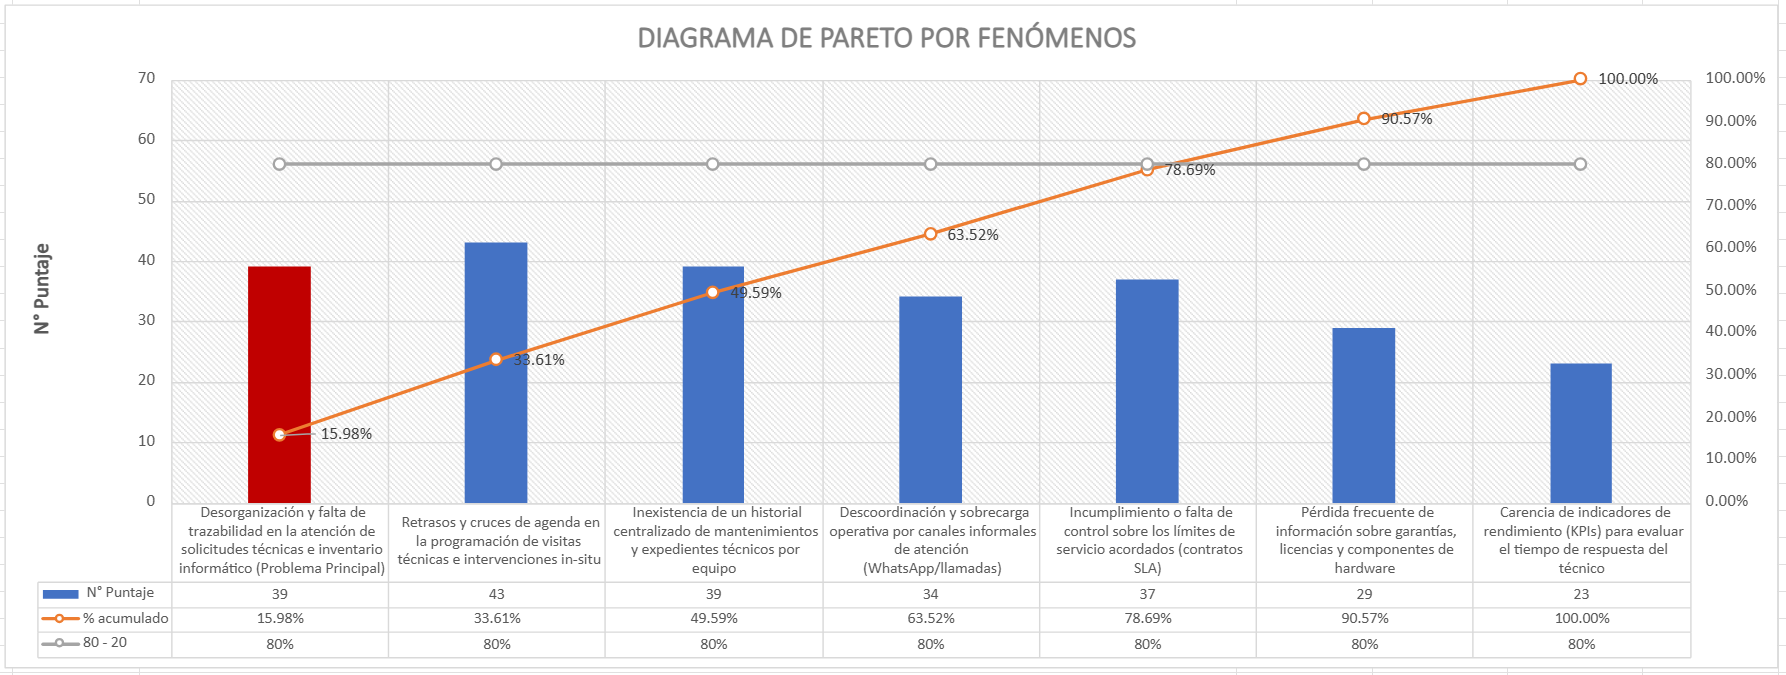
\includegraphics[width=1\linewidth]{img/diagrama_pareto.png} \\[0.2em]

\raggedright
{\small \textit{Nota.} Representación gráfica de la regla 80/20 que evidencia las causas principales a resolver en la gestión del HelpDesk.}
\end{figure}


\clearpage
\phantomsection\label{anexo4}
\hypertarget{anexo4_acta}{}

\noindent \textbf{Anexo 4}
\vspace{0.4em}

\begin{figure}[H]
    \centering
    \caption{Acta de Constitución del Proyecto (Parte 1)}
    \label{fig:acta_constitucion_1}
    \vspace{0.3em}
    \raggedright
    \textbf{Figura A.2} \\
    \textit{Acta de Constitución del Proyecto (Parte 1)} \\[0.3em]
    \centering
    % trim = [izquierda, abajo, derecha, arriba] en puntos (pt). Ajusta los valores si necesitas más o menos recorte.
    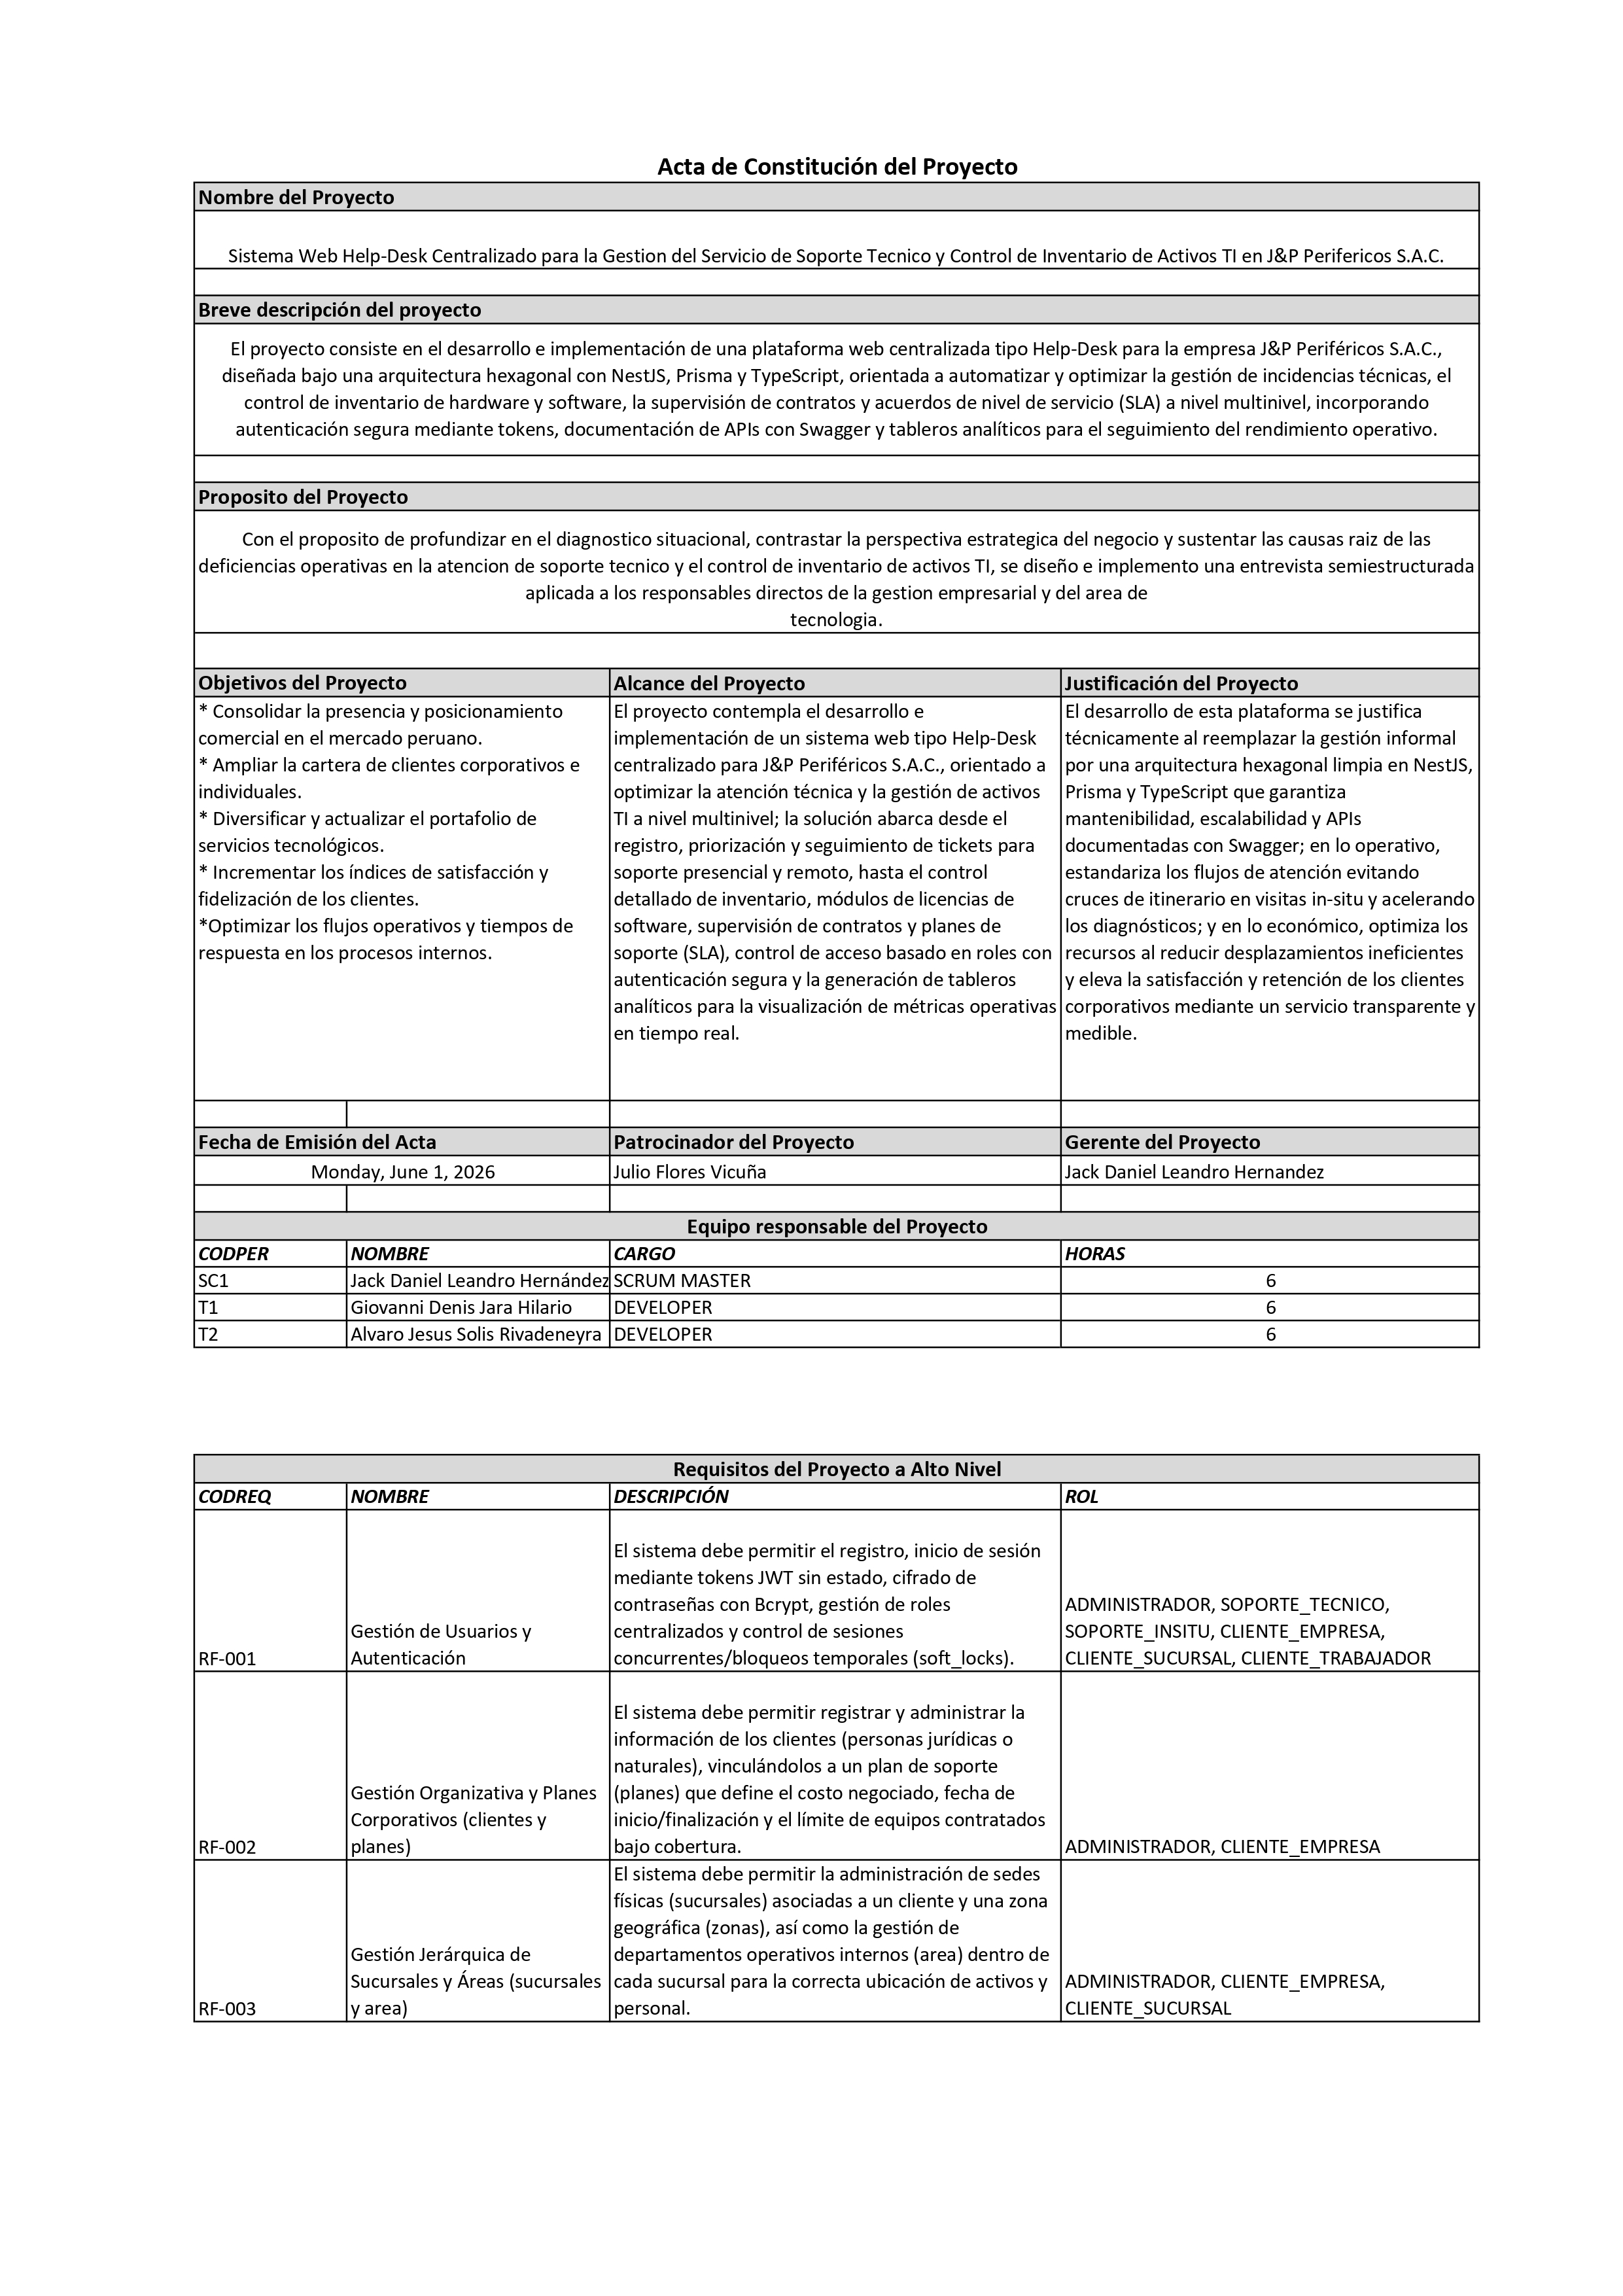
\includegraphics[width=0.82\linewidth, trim=0 80 0 40, clip]{img/Acta_Constitucion_HelpDesk_page_01} \\[0.3em]
    \raggedright
    {\small \textit{Nota.} Documento oficial de constitución, objetivos, alcance y equipo responsable de J\&P Periféricos S.A.C.}
\end{figure}

\clearpage

\begin{figure}[H]
    \centering
    \caption{Acta de Constitución del Proyecto (Parte 2)}
    \label{fig:acta_constitucion_2}
    \vspace{0.3em}
    \raggedright
    \textbf{Figura A.3} \\
    \textit{Acta de Constitución del Proyecto (Parte 2)} \\[0.3em]
    \centering
    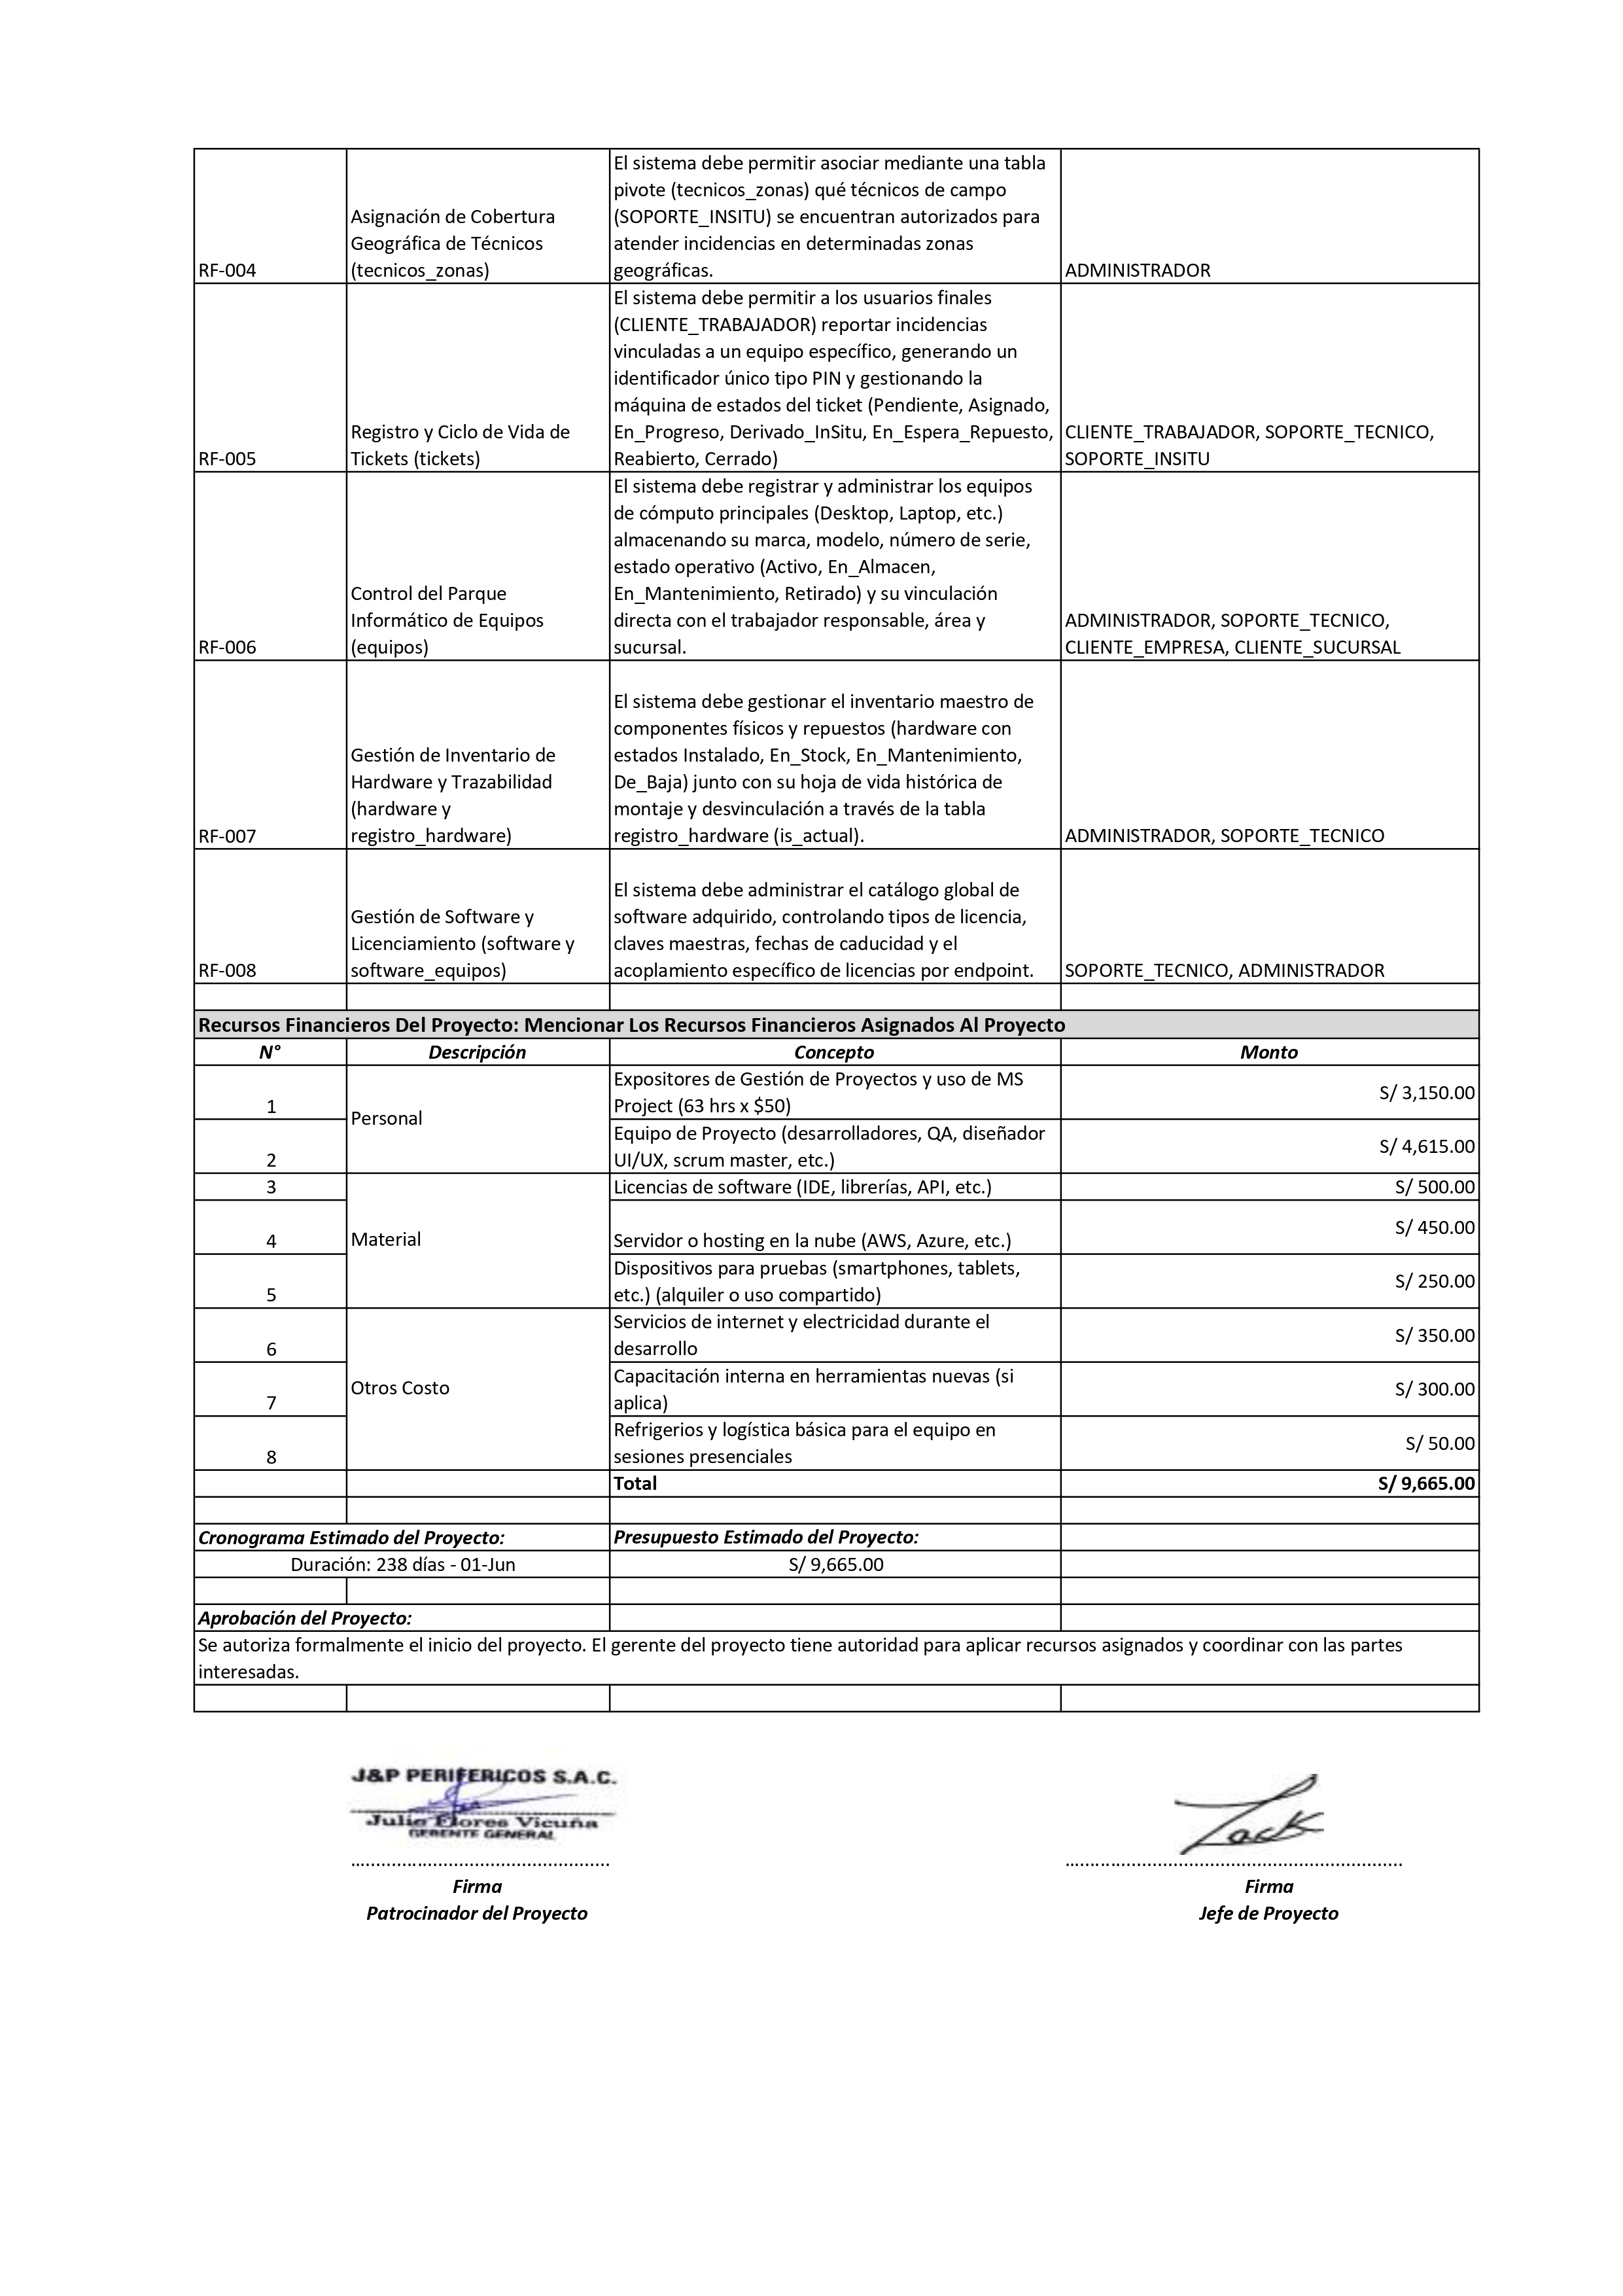
\includegraphics[width=0.82\linewidth, trim=0 120 0 40, clip]{img/Acta_Constitucion_HelpDesk_page_02} \\[0.3em]
    \raggedright
    {\small \textit{Nota.} Detalle de requerimientos a alto nivel, recursos financieros, cronograma y firmas de aprobación del proyecto.}
\end{figure}

\end{document}